\ustcsetup{
  cite-style = authoryear,
}

\chapter{基于MCMC方法的震源参数评估方法}

\section{引言}

在早期震源模型的研究中,单力偶模型最先被提出并用于解释观测到的P波初动符号\citep{nakano1923notes};
随后地震学家们发现无矩双力偶模型也能正确解释P波初动符号,并且满足角动量守恒,是更合理的震源模型\citep{honda1957mechanism}。
Burridge 和 Knopoff \citep{Burridge1964}将等效体力的概念引入到震源模型中,
证明了连续介质内部震源区的一组体力辐射出的位移场与断层面上的位移间断辐射出的位移场等价。
随后地震矩张量的概念被提出,其可以看做是等效体力的一阶近似,是描述震源区时间和空间的函数,并且成功解释了位错源与体积源模型。
地震矩张量逐渐被地震学家们广泛接受,并成为现代地震学对震源描述的一种标准。

地震震源参数的研究是震源研究的核心之一,基于波形拟合的方法被广泛应用到震源反演中。
震源参数反演主要由两部分组成,地震定位与震源机制反演,
通常先进行地震定位,再利用定位的位置进行震源机制反演。
这两部分都是很强的非线性反演问题。
传统的两步反演方法容易收到累积误差的影响,即第一步地震位置的误差被传入到第二步震源机制的反演中,
进而影响第二步震源机制的反演\citep{Tan2018}。
因为测量误差与随机噪声的存在,反演的不确定性是真实存在的,同时不确定性评估也是反演结果评价的一个重要方面。
然而,传统的方法,例如广泛使用的网格搜索与最小二乘等,通常只会提供一个最优解,并不能提供结果的不确定性评估。

马尔科夫蒙特卡洛(Markov Chain Monte Carlo,简称MCMC)是一种全局优化方法,
其基于贝叶斯统计理论,对参数模型空间的后验概率(posterior probability density,简称PDD)进行采样,
获得参数模型的不确定性评估信息。
MCMC方法已经被应用到许多非线性反演问题中。
近些年,一些学者提出并编写了许多开源的程序包,用于震源参数的贝叶斯反演,
例如BayesISOLA\citep{Vackaar2017}, MTfit\citep{Pugh2018},GBIS\citep{Bagnardi2018},和 BEAT\citep{Vasyura-Bathke2020}。
然而,MCMC的方法通常对先验模型有很强的依赖性,一些早期开发的程序包没有和现在流行的地震学编程环境进行交互,
例如ObsPy\citep{Beyreuther2010} 和 ASDF\citep{Krischer2016}。

在本文研究中,我们将展现一个新的程序包MCMTpy进行震源参数反演,
该程序包基于贝叶斯统计理论与CAP算法,由Python语言编写。
MCMTpy使用马尔科夫链去串联传统的两步反演方法,基于P波和S波相位到时信息反演震源位置与
利用波形信息反演震源机制,并使其成为一个反演流程。
新的方法可以同时反演地震震级、水平位置、震源深度、发震时刻和震源机制(双力偶与矩张量)。
我们将该方法应用到2021年中国云南漾濞地震与2008年美国Mt. Carmel地震反演中,
并成功获得了主震双力偶模型与矩张量模型的震源机制解。
我们通过设置30个不同的初始模型探讨了该方法的鲁棒性,并讨论其潜在的应用。

本章,我们将首先介绍相关的震源理论,包括震源理论,与常用的震源机制反演方法。
然后提出新方法MCMTpy的原理,并介绍其在两次地震中的应用,并进行相关讨论。







\section{震源理论}

地震震源的数学描述是复杂的,20世纪中后期,地震学家将“矩张量”引入到震源理论中,进而统一了争论已久的震源模型。
震源模型通常分为两类:适用于中小地震的点源模型,与适用于大地震的非点源模型。
根据近似程度的不同又可进一步分为:单力偶模型、双力偶模型、矩张量模型、二阶矩张量模型(或FMT有限矩张量模型)、多点源模型与有限破裂模型等。
其模型参数逐渐增加。
本节我们聚焦于震源模型的理论推导,主要参考文献为定量地震学\citep{aki2002quantitative}。
我们从运动方程出发,推导出点源模型、高阶矩张量模型与有限断层模型的震源表达式;
并介绍矩张量分解的一般方法,与矩张量可视化的方法。

\subsection{震源模型与矩张量}

\subsubsection{运动方程}
在连续介质的假设下,根据\citep{aki2002quantitative}给出的运动方程(The Equation of Motion),有方程:
\begin{align}
    \rho {\ddot \mu_i} & = f_i + \tau_{ji,j} \notag \\
    T_i & = \tau_{ij} n_j
    \label{equ:motion-1}
\end{align}
其中$\rho$单位体积的密度,$i,j$表示不同分量,$\mu$是位移,$f$是作用于单位体积介质上的体力(主要包括重力与其他外力等;一般情况重力可以忽略,在研究自由振荡时需要考虑重力),
$\tau$应力张量,$T$是牵引力(traction)。



\subsubsection{Betti互易定理}

假设存在两个力系。第一个力系中,$u=u(x,t)$表示位移场,由体力$f$、$S$面上的边界条件和初始时刻$t=0$条件唯一确定,牵引力用$T(u,n)$表示,其中$n$是平面法向向量;
第二个力系中,$v=v(x,t)$表示位移场,由体力$g$、$S$面上的边界条件和初始时刻$t=0$条件唯一确定(注意此条件一般与$u$中的条件不同),牵引力用$T(v,n)$表示;

根据公式~\ref{equ:motion-1},我们可以得到Betti第一互易定理:
\begin{align}
    & \iiint\nolimits_V (f - \rho {\ddot \mu})\cdot v \,dV + \iint\nolimits_S T(u,n) \cdot v \,dS \notag \\
    = & \iiint\nolimits_V (g - \rho {\ddot v})\cdot u \,dV + \iint\nolimits_S T(v,n) \cdot u \,dS 
    \label{equ:betti-1}
\end{align}

Betti第二互易定理可以轻松由第一互易定理得到:

\begin{align}
    & \int\nolimits_{-\infty}^\infty \,dt \iiint\nolimits_V \{ u(x,t) \cdot g(x,\tau-t) -v(x,\tau-t) \cdot f(x,t) \} \,dV  \notag \\
    = & \int\nolimits_{-\infty}^\infty \,dt \iint\nolimits_S \{ v(x,\tau-t) \cdot T(u(x,t),n) - u(x,t) \cdot T(v(x,\tau-t),n) \}  \,dS
    \label{equ:betti-2}
\end{align}

\begin{figure}[h]
    \centering
    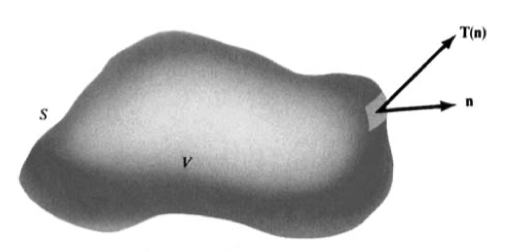
\includegraphics[width=0.9\textwidth]{source/betti.jpg}
    \caption{体积为$V$的连续体,表面用$S$表示}
    \label{fig:betti}
    \note{注:图片引自\citep{aki2002quantitative}}
\end{figure}

\subsubsection{位移表示定理}

从Betti第二定理出发,如果我们将其中一个力系的体力用$\delta$函数表示,那么其对应的位移场就是格林函数(格林函数的定义);
此时第二个位移场就可以用格林函数表示出来,即为位移表示定理。

假设我们想获得体力为$f$(连续体$V$边界条件为$S$)的位移$u$。
我们令另一体力$g_i(x,t)=\delta_{in} \delta(x-\xi) \delta(t)$,
其对应的位移场$v_i(x,t)=G_{in}(x,t;\xi,0)$,
带入Betti第二定理(公式~\ref{equ:betti-2}),并交换$x$和$\xi$、$t$和$\tau$,获得:

\begin{align} 
    u_{n}(\mathbf{x}, t) = & \int\nolimits_{-\infty}^{\infty} d \tau \iiint\nolimits_{V} f_{i}(\xi, \tau) G_{i n}(\xi, t-\tau ; \mathbf{x}, 0) d V(\xi) \notag \\ 
     + & \int\nolimits_{-\infty}^{\infty} d \tau \iint\nolimits_{S} \{ G_{i n}(\xi, t-\tau ; \mathbf{x}, 0) T_{i}(\mathbf{u}(\xi, \tau), \mathbf{n}) \notag \\ 
     & \qquad -  u_{i}(\xi, \tau) c_{i j k l} n_{j} G_{k n, l}(\xi, t-\tau ; \mathbf{x}, 0) \} d S(\xi) 
\end{align}

这就是位移第一表示定理。




\subsubsection{震源表示定理}

通常由于外部作用引起的地震波,如风、海浪、陨石撞击、大气层爆炸甚至人为活动,是容易建立物理数学模型进行分析的。
但对于其他震源活动,如火山喷发、核爆与天然地震等,它们属于内部源;因为运动方程(方程~\ref{equ:motion-1})不能在整个地球内成立(震源区不成立),所以传统的框架很难建立。

考虑两种极端情况下的震源类型,发生在平面上的断层破裂与地下的爆炸,
它们的联系是,在内部平面上的位移不连续(断层破裂)与某体积内的应变不连续(体积元膨胀)。
注意:如果是自发破裂(没有外力的作用),根据牛顿第三定理,地下的应力始终的连续的。

用统一的数学语言来描述上述模型,地震学家们有两种选择:第一,用体力来表示震源区介质的情况;
第二,通过地下某平面上的位移不连续或者某体积内的应变不连续,来描述震源。
经过证明,我们发现第二种方案可以解释第一种方案,其关键点将位移与应变不连续解释为等效体力的概念\citep{Burridge1964}。

\begin{figure}[h]
    \centering
    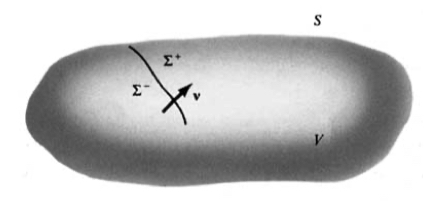
\includegraphics[width=0.9\textwidth]{source/source-cartton.jpg}
    \caption{内部源模型}
    \label{fig:source-cartton}
    \note{注:一个有限体积的弹性体,外表面是$S$,内表面是$\Sigma$(例如表示一个内部断层)。
    内表面是不连续点的边界,并分为两面,分别是$\Sigma^-$和$\Sigma^+$。
    $v$是内表面的法向向量,从$\Sigma^-$指向$\Sigma^+$。
    $[u(\xi,\tau)]$表示$\Sigma$面上的位移不连续,方括号表示运算符 $u(\xi,\tau)|_{\Sigma^+} - u(\xi,\tau)|_{\Sigma^-}$。
    对于自发破裂,牵引力是连续的,所以$[T(u,v)]=0$。
    图片引自\citep{aki2002quantitative}}
\end{figure}

我们构建内部源的几何模型(图~\ref{fig:source-cartton}),此时边界包含两部分:外部面$S$与内部两个互相相接的面$\Sigma^-$和$\Sigma^+$。
因为我们更关系内部源发生的物理过程,外部面$S$(可以看做地球表面)不再是我们研究主要对象,所以我们假设位移场$u$与格林函数$G$在$S$上都满足齐次边界条件(对应的二元面积分为0)。
带入位移表示定理并简化:
\begin{align}
    u_{n}(\mathbf{x}, t)=& \int\nolimits_{-\infty}^{\infty} d \tau \iiint\nolimits_{V} f_{p}(\eta, \tau) G_{n p}(\mathbf{x}, t-\tau ; \eta, 0) d V(\eta) \notag \\
    +  & \int\nolimits_{-\infty}^{\infty} d \tau \iint\nolimits_{\Sigma} \{ [u_{i}(\xi, \tau) c_{i j p q} v_{j} \partial G_{n p}(\mathbf{x}, t-\tau ; \xi, 0) / \partial \xi_{q}] \notag \\
    & \qquad - [G_{n p}(\mathbf{x}, t-\tau ; \xi, 0) T_{p}(\mathbf{u}(\xi, \tau), \nu) ] \} d \Sigma .
    \label{equ:source-raw}
\end{align}
其中$\eta$表示体积体$V$内的任意一点,$\xi$表示不连续面$\Sigma$上的任意一点,$p,q,n$表示方向。
注意Betti互易定理与位移表示定理都只适用于连续介绍,但现在我们需要考虑不连续面的存在,似乎此时表示定理不满足成立条件。
但是此时模型不再简单地视为单连通体,而是将不连续面看做是复连通体的内边界,我们依然可以将几何模型(图~\ref{fig:source-cartton})看成连续介质\citep{Nabarro1951}。
我们可以对上述公式~\ref{equ:source-raw}进一步化简:首先在不考虑地球自由震荡的情况下,体力$f$(例如重力)可以不考虑,将其值设为0;
因为断层面的相对滑动会产生位移,所以$[u]$不等于零;
因为牵引力的连续性,所以$[T(u,v)]=0$;
格林函数$G$在面$\Sigma$上是连续可导的;最后可以简化为:
\begin{align}
    u_{n}(\mathbf{x}, t)= \int\nolimits_{-\infty}^{\infty} d \tau \iint\nolimits_{\Sigma}  [u_{i}(\xi, \tau)] c_{i j p q} v_{j} \frac{\partial}{\partial {\xi_q}} G_{n p}(\mathbf{x}, t-\tau ; \xi, 0)  d \Sigma 
   \label{equ:source-rep}
\end{align}
其中$[u(\xi,\tau)]$称之为滑动函数(slip function);该公式就是震源表示定理,基于它发现了一系列简化震源研究的方法;
我们可以发现,只需要知道断层面上的位移,就可以确定整个空间上位移场信息。


\subsubsection{位错模型的等效体力}
分析震源表示定理(公式~\ref{equ:source-rep}),我们发现尽管在推导过程中,没有直接显示地包含体力的影响(即体力导致在断层面上的位移,进而控制整个空间的位移场)。
但我们发现确实在用$(x,t)$上的位移与格林函数做积分;
如果我们创建一种虚拟的力,与力与格林函数在断层面上做积分的效果一致,我们称之为等效体力(body-force equivalent)。
回顾公式~\ref{equ:source-raw}的右边三项,可以将后两项的面积分通过高斯定理转变为体积分,转换后的积分内部函数应该与第一项的内部函数的单位一致,即与$f_p$单位一致。
下面我们推导位移不连续项的等效体力表示,格林函数$G$的偏导可以用$\delta$函数在整个空间积分表示:
\begin{align}
    \frac{\partial}{\partial {\xi_q}} G_{n p}(\mathbf{x}, t-\tau ; \xi, 0) =
     \iiint\nolimits_{V} \frac{\partial}{\partial {\eta_q}} \delta(\eta-\xi) G_{np}(x,t-\tau;\eta ,0) dV(\eta ) 
   \label{equ:int_gf}
\end{align}
所以位移不连续项在公式~\ref{equ:source-raw}可表示为:
\begin{align}
    u_{n}^{disp}(\mathbf{x}, t)=
    \int\nolimits_{-\infty}^{\infty} d \tau \iiint\nolimits_{V} 
    \biggl\{ -\iint\nolimits_{\Sigma}  [u_{i}(\xi, \tau)] c_{i j p q} v_{j}  \frac{\partial}{\partial {\eta_q}} \delta(\eta-\xi) d\Sigma \biggl\}
        G_{n p}(\mathbf{x}, t-\tau ; \eta , 0) dV
    \label{equ:source_disp}
\end{align}
位移不连续的等效体力可以表示为:
\begin{align}
    f_p^{[u]}(\eta ,\tau) = 
    -\iint\nolimits_{\Sigma}  [u_{i}(\xi, \tau)] c_{i j p q} v_{j}  \frac{\partial}{\partial {\eta_q}} \delta(\eta-\xi) d\Sigma
    \label{equ:bf-equ}
\end{align}

同理应力张量的不连续(注意:在研究自发破裂的内部源时,我们通常假设没有应力间断)也可以表示成等效体力,这里省略证明。
因为这是内部源破裂的过程,所以该过程的动量与角动量应保持不变,所以任何等价体力要满足下述两个方程:
\begin{align}
    \iiint\nolimits_V  f_p^{[u]}(\eta ,\tau) dV(\eta ) & = 0  \qquad \text{for all } \tau \\
    \iiint\nolimits_V  (\eta-\eta_0) \times f_p^{[u]}(\eta ,\tau) dV(\eta ) & = 0  \qquad \text{for all } \tau \text{ and any fixed } \eta_0
\end{align}

证明可参考定量地震学\citep{aki2002quantitative}。
等效体力在地震学中最重要的应用是平面剪切位错的断层模型。
但它不能表示作用在任何介质上真实地力,只是它的效果与位错引起地震辐射相同,所以是其等效力。
通过等效体力的表达式~\ref{equ:bf-equ}可以推导出著名的地震矩(seismic moment)表达式,这里直接给出结论:
\begin{align}
    M_0 = \mu \bar{u} A = \mu \times  \text{[average slip]} \times \text{[fault area]}
\end{align}
其中$M_0$是地震矩,它描述了地震断层滑动的强度。其量级变化巨大,例如大地震$M_0$大约在 $10^{30} dyne$(例如 1964 Alaskan earthquake),
一些小地震约为$10^{12} dyne$,实验室实验产生的微破裂大约$10^{5} dyne$。
量级的巨大差异对地震学家的研究是不利的,Kanamori在1977年\citep{Kanamori1993}引进了矩震级$M_w$的概念:
\begin{equation}
    log_{10}(M_0)  = 1.5M_w + 16.1
\end{equation}
$M_w$也是现代震级最常用的概念。



\subsubsection{位错源模型的矩张量}
上一节我们用等效体力的概念解释了位错源,Backus 和 Mulcahy \citep{Backus1976a} 指出除了等效体力外也可以用矩张量密度来描述,
并进一步推广了地震矩张量的概念,这些概念在解释非剪切位错源时也更加容易理解。
回顾公式~\ref{equ:source-rep},利用卷积符号$\ast$取代最外层积分符号变成时间域的卷积,可以得到:
\begin{align}
    u_{n}(\mathbf{x}, t)= \iint\nolimits_{\Sigma}  [u_{i}(\xi ,t)] c_{i j p q} v_{j} \ast \frac{\partial}{\partial {\xi_q}} G_{np}  d \Sigma 
   \label{equ:source-rep-m}
\end{align}
注意$f \ast g = \int\nolimits_0^t f(\tau)g(t-\tau) d\tau = \int\nolimits_0^t f(t-\tau)g(\tau) d\tau = \int\nolimits_{-\infty}^{\infty} f(\tau)g(t-\tau) d\tau$
如果$f(t)$和$g(t)$当$z<0$时都等于零。
我们定义地震矩张量密度为:
\begin{align}
    m_{pq}(\xi ,t)=[u_i(\xi ,t)]v_j c_{ijpq}
    \label{equ:moment-density-tensor}
\end{align}
震源表示定理可进一步写为
\begin{align}
    u_{n}(\mathbf{x}, t)= \iint\nolimits_{\Sigma} m_{pq}(\xi ,t) \ast  G_{np,q} (\mathbf{x}, t; \xi, 0) d \Sigma 
   \label{equ:source-rep-mdt}
\end{align}
$\xi$表示不连续面$\Sigma$上的某一位置;当不连续面$\Sigma$的长度(震源尺度)远小于观测距离$x$时,我们可以把地震当成点源,
此时格林函数中的变量$\xi$可以看成常量考虑,那么可以将格林函数$G$从积分里面提出来:
\begin{align}
    u_n(x,t)=M_{pq}(t)*G_{np,q}
    \label{equ:U-M*G}
\end{align}
其中$M_{pq}$是地震矩张量密度$m_{pq}$在整个不连续面上$\Sigma$的积分,
\begin{align}
    M_{pq} = \iint\nolimits_{\Sigma} m_{pq} d{\Sigma} 
    = \iint\nolimits_{\Sigma} [u_i]v_j c_{ijpq} d{\Sigma}
    \qquad \text{i.e.,} \qquad
    m_{pq}=\frac{dM_{pq}}{d\Sigma}
    \label{equ:M-m}
\end{align}
假设地震矩张量的各个分量随时间变化是同步的,则有:
\begin{align}
    M_{pq}(t)=M_{pq}S(t)
    \label{equ:s-t-f}
\end{align}
其中$M_{pq}$称为静态地震矩张量,$S(t)$为震源时间函数(source time function)。
此时我们获得了最常用地震学表达式:
\begin{align}
    u_n(x,t)=M_{pq}S(t)*G_{np,q}
    \label{equ:U-MS*G}
\end{align}

本节小结:我们定义了位错源下的矩张量密度公式,发现位错源假设下位移场可以由矩张量与格林函数的卷积表示。



\subsubsection{体积源模型的矩张量}
前面几节我们讨论了位错源模型下,震源可以用等效体力与矩张量密度来表示;本节我们将探讨,对于体积源模型(地下爆炸)的震源表示理论。
我们需要引入转换应变(transformational strain),也称无应力应变,来描述体积源。
根据\citep{eshelby1957determination}提出的模型进行说明。该模型主要分为5个步骤:

\begin{enumerate}
\item 假设在空间$V$中,震源体与周围物质以$\Sigma$面间隔,我们首先沿$\Sigma$面切割并将震源体 
移出。假设被移出震源体的表面$\Sigma$上的应力不变,从而使其保持原有状态。
\item 我们给震源体添加转换应变$\Delta e_{rs}$,但不改变震源体内的应力,该应变也称之为无应力应变(stress-free strain)来描述体积源。
该应变描述了震源过程,例如相变、热膨胀或者塑性变形等。
\item 我们在震源体外表面施加力,使震源体恢复到没发生应变的状态,其结果是在震源体内产生一个附加应力场
$-c_{pqrs} \Delta e_{rs} = -\Delta \tau_{pq}$,此时其在震源体外表面$\Sigma$上的附加应力变成 $-c_{pqrs} \Delta e_{rs} v_q$,
$v_q$是$\Sigma$面上指向外的法线向量。并且由于$\Delta \tau_{pq}$是静态场,所以$\Delta \tau_{pq,q}=0$。
\item 我们把经过应变的震源体放回到空间$V$中的原来位置(与原来的形状保持一致),此时发现$\Sigma^-$面上的应力比$\Sigma^-$上的大了 $-c_{pqrs} \delta e_{rs} v_q$,
此时会造成在面$\Sigma$上应力的间断。
\item 我们解除施加在震源体外表面的力,此时相当于恢复到最原始状态但震源体内多增加了转换应变。
此时穿过$\Sigma$面的应力是连续的。
\end{enumerate}
上述过程说明震源体发生转换应变$\Delta e_{rs}$(例如膨胀爆炸)的效果与在面$\Sigma$上产生大小为$-c_{pqrs} \Delta e_{rs} v_q$的应力间断作用是一致的。
所以在周围物质里传播的地震弹性波可以看成是由于$\Sigma$面的视应力间断造成的。

我们假设应力间断为$[T_p]=-c_{pqrs} \Delta e_{rs} v_q$,带入到震源表示定理,并不考虑外力项与位移间断项:

\begin{align}
    u_{n}(\mathbf{x}, t)= \int\nolimits_{-\infty}^{\infty} d \tau \iint\nolimits_{\Sigma}  c_{pqrs} \Delta e_{rs} v_q  G_{n p}(\mathbf{x}, t-\tau ; \xi, 0)  d \Sigma(\xi) 
   \label{equ:source-T0}
\end{align}
使用高斯定理将面积分转换为体积分:
\begin{align}
    u_{n}(\mathbf{x}, t)= \int\nolimits_{-\infty}^{\infty} d \tau \iiint\nolimits_{V}  \frac{\partial}{\partial {\xi_q}} 
    \biggl\{ c_{pqrs} \Delta e_{rs}   G_{n p}(\mathbf{x}, t-\tau ; \xi, 0) \biggl\}
     dV(\xi) 
   \label{equ:source-T1}
\end{align}
注意公式~\ref{equ:source-T1}里的$V$表示震源体,不是全空间。因为$\partial(c_{pqrs} \Delta e_{rs})/\partial \xi_q = \Delta \tau_{pq,q} = 0$,上式可以简化为:
\begin{align}
    u_{n}(\mathbf{x}, t)=  \iiint\nolimits_{V}   
    c_{pqrs} \Delta e_{rs} \ast  \frac{\partial G_{n p}}{\partial {\xi_q}} 
    dV 
   \label{equ:source-T2}
\end{align}
比较上述公式~\ref{equ:source-T2}与公式~\ref{equ:source-rep-mdt},我们可以类似地引入一个矩密度张量:
\begin{align}
    \frac{\partial M_{pq}}{\partial V} = c_{pqrs} \Delta e_{rs} 
   \label{equ:moment-tensor-T}
\end{align}
单位体积上的矩在整个震源区积分就是位移场:
\begin{align}
    u_{n}(\mathbf{x}, t)=  \iiint\nolimits_{V}   
    \frac{\partial M_{pq}}{\partial V} \ast  \frac{\partial G_{n p}}{\partial {\xi_q}} 
    dV 
   \label{equ:source-T3}
\end{align}
需要注意$\Delta \tau_{pq} = \partial M_{pq}/dV$不是应力降(stress drop)。
因为应力降不只局限于震源体内,而$\Delta \tau_{pq}$只存在于震源体上,我们成$\Delta \tau_{pq}$是应力过剩(stress glut)\citep{Backus1976b}。
当震源体的体积$V$很小,可以将其视为点源,那么矩张量可以表示成:
\begin{align}
     M_{pq} =  \iiint\nolimits_{V} c_{pqrs} \Delta e_{rs}  dV 
   \label{equ:source-T4}
\end{align}
此时公式~\ref{equ:source-T3}可进一步简化为:
\begin{align}
    u_n(x,t)=M_{pq}*G_{np,q}
    \label{equ:T-U-M*G}
\end{align}

本节小结:我们通过引入无应力应变(或转换应变)的概念,证明了体积源产生的位移场可以看成是视应力间断造成了,
该视应力间断也称应力过剩(stress glut)。
体积源位移场可以直接由无应力应变张量或者应力过剩张量描述,我们定义了矩张量密度(公式~\ref{equ:moment-tensor-T})公式,
发现体积源的震源表示定理与位错源的震源表示定理相一致。






\subsubsection{等效体力、矩张量密度、无应力应变和应力过剩的相互关系}

内部地震源可以用一个矢量场或三种对称二阶张量场中的任意一种来描述。
矢量场是等效体力场。
张量场包含无应力应变,应力过剩,以及任何其他的矩张量密度。
在推导位错源时引入了等效体力的概念,并引入了矩张量密度。
在推导体积源时引入了无应力应变和应力过剩的概念,并引入了矩张量密度。
内部地震源也可以用四种描述中的任意一种泰勒展开多项式的矩来描述,对于近乎于点源假设的情况,
可以用等效体力或应力过剩的有限的低阶矩来描述。
\paragraph{矩张量与等效体力}
之前我们定义位错源下的等效体力表达式,需要强调等效体力$f$是单位空间上的力。
我们可以进一步发现,无论在位错源还是体积源假设下,矩张量与等效体力存在以下关系:
\begin{align}
    M_{pq} =  \iiint\nolimits_{V} f_p \eta_q dV(\eta)
  \label{equ:moment-tensor-with-eq}
\end{align}
该公式可以进一步拓展矩张量$M$的定义,它可以描述空间中任何等效体力的分布,而不仅仅是位移间断模型下的等效体力。
在点源的假设下,地震矩张量是等效体力的一阶矩张量。

\paragraph{矩张量与无应力应变和应力过剩}
在点源的假设下,地震矩张量是应力过剩或任意矩张量密度的零阶矩张量。
正是基于矩张量在各种情况下的适用性,地震学家改变了传统研究震源的方式,开辟了用矩张量描述震源的新领域。








\subsection{等效体力的矩张量展开}

上一节我们根据两种特定类型的震源模型,位错源与体积源,推导了他们的矩张量表达形式。
现代物理学的出发点是力,一切自然现象都可以用力的形式进行数学物理描述,地震现象也不例外。
本节我们在等效体力的框架下,建立地震破裂的一般模型。


\subsubsection{破坏过程}

在物理上,地震涉及某种非线性破坏过程,如断裂或摩擦滑动,其作用在一个有限的区域内。
作用于整个(无断层)模型介质中的等效力系,会在源区域外产生相同的位移场。
因为等效体力系统是可以从位移场中反推出来的,所以它是一种对震源的描述。
任何物理源都有一个独特的等效力系统;但反之不然,许多不同的物理过程可能具有相同的力系统,因此具有相同的静态和动态位移场。
正因为等效力系统和物理源过程之间的对应关系是一对多的,因此等效力系统(地震和大地观测等方法)不能唯一地确定物理源过程。
最熟悉的例子是断层面和与之正交的“辅助面”之间的模糊性,其中任何一个断层面都会产生相同的地震波辐射。

破坏过程可以看作是本构关系(应力-应变规律)的突然局部变化\citep{Backus1976a},即在震源区以胡克定律为例的本构关系不再成立。
发生破坏前,应力场满足平衡方程。
在破坏时,本构关系的快速变化导致应力场的变化,因此辐射出弹性波运动。
在下面的讨论中都不考虑重力的影响,在无外力的情况下,运动方程为:
\begin{align}
    \rho \ddot u_i = \sigma_{ij,j} 
  \label{equ:motion}
\end{align}
其中$\rho(x)$是密度函数,$u(x,t)$的位移场,$\sigma(x,t)$是介质的应力张量,$x$表示位置,$t$表示时间,$j$下标表示对该分量的微分。
然而在发生破坏过程时,真实的$\sigma(x,t)$往往是未知的,但我们通过本构关系中的胡克定律(Hooke's law)可以知道理论上的应力,记为$s(x,t)$。
如果我们用$\sigma_{ij}$取代$s_{ij}$带入运动方程(公式~\ref{equ:motion}),我们必须引入另外一个力$f(x,t)$来让等式成立:
\begin{align}
    \rho \ddot u_i = s_{ij,j} + f_i
  \label{equ:f-motion}
\end{align}
我们定义$f_i = {(\sigma_{ij} - s_{ij})}_{,j}$,是地震的等效体力密度。它在震源区外的地方是零。
Backs 和 Mulcahy (1976a b)将真实情况下应力与模型理论应力的差值定义为应力过剩(stress glut)。


\subsubsection{矩张量}
给定等效力系统$f(x, t)$,计算地球的位移场是一个线性问题,其解可以表示为对震源区域$V$的积分
(为简便起见,忽略位移和牵引间断点,因为它们也可以表示为对应的等效体力):
\begin{align}
    u_i(x,t) = \iiint\nolimits_V G_{ij}(x,\xi,t) \ast f_j(\xi,t) d^3\xi
  \label{equ:u-f}
\end{align}
其中$G_{ij}(x,\xi,t)$是格林函数,它给出了位置$x$和时间$t$的位移的第$i$个分量,
由施加在震源区位置$\xi$和时间$t$的第j个方向的力$f_j$引起。
这是震源表示定理的等效体力形式,现代许多教科书直接从此公式出发,推导后续的矩张量。
通常震源区的尺度$\xi$是一定的,我们可以将格林函数在震源位置$\xi$处做泰勒展开:
\begin{align}
    G_{ij}(x,\xi,t)  = G_{ij}(x,0,t) + G_{ij,k}(x,0,t)\xi_k + \dots
  \label{equ:G-taylor}
\end{align}
所以公式~\ref{equ:u-f}可以写成:
\begin{align}
    u_i(x,t) = G_{ij}(x,0,t) \ast F_j(t) + G_{ij,k}(x,0,t) \ast M_{jk}(t) + \dots
  \label{equ:u-f-T}
\end{align}
其中震源激发的总力为$F_j(t)$,根据震源过程的动量守恒,该项通常假设为零:
\begin{align}
    F_j(t) = \iiint\nolimits_V  f_j(\xi,t) d^3\xi
  \label{equ:F0}
\end{align}
矩张量定义为:
\begin{align}
    M_{jk}(t) =  \iiint\nolimits_{V} \xi_k f_j(\xi,t)  d^3\xi
  \label{equ:mt-eq}
\end{align}
矩张量是一个二阶张量,它描述了九个基本力系的叠加,每个张量的分量表示一个力系的强度(矩)。
对角线分量$m_{11},m_{22},m_{33}$对应的是没有力矩的线性偶极子,
而非对角线分量$m_{12},m_{13},m_{21},m_{23},m_{31},m_{32}$对应的是力偶。
通常假设力矩张量是对称的,所以力偶不施加净力矩,在这种情况下只有6个独立的力矩张量分量。
对于一个对称的,六元矩张量我们总是可以选择一个由三个正交线性偶极子组成的坐标系,所以矩张量是对角的。
换句话说,一般的点源可以用三个值(主矩)来描述它的物理特性,以及三个值来描述它的方向。

% 矩张量有三个重要的性质,使得它可以用来表示震源。
% \begin{enumerate}
% \item 使理论地震波激励计算的“正问题”线性化。一般的震源被表示为各等效力系的加权和,因此任何地震波都只是由不同震源激发的波的加权和。
% 正问题的线性反过来使从观测中确定源机制的反问题更加容易处理。
% \item 简化了波浪激励的计算。通过将矩张量转换为一个适当定向的坐标系,可以使定义观测方向的角度具有特殊值,如0和p/2。
% 因此,基本源的辐射不用在一般具体方向上计算,可以在计算比较容易的几个方向上计算。
% 例如,在横向均匀介质中,只需要计算一个方位角的辐射。
% \item 矩张量比直流表示更普遍。它包括DC作为特殊情况,但比DC多两个自由参数(6个和4个),这使它能够表示涉及体积变化的源和比平面上的简单滑移更常见的剪切类型。
% 正是这种普遍性使得矩张量表示在研究非双力偶地震中很重要。
% \end{enumerate}



\subsubsection{矩心矩张量}
震源表示定理将地震表示为一个点源,那么点源的位置究竟在哪里,也就是说公式~\ref{equ:G-taylor}究竟在震源什么位置进行泰勒展开。
由定义可知,如果总力消失,那么常规的二阶矩张量与原点无关。(然而,实验确定的矩张量可以依赖于原点,因为格林函数依赖于假设的源位置。)
质心具有以下特性:(1)第一个力矩消失(通常假设),(2)使第二个力矩最小(在质量的情况下是惯性矩,在概率的情况下是方差)。
Backus\citep{backus1977interpreting} 建议将质心定义为在最小二乘意义上使二阶矩最小的点。
这样定义的质心在空间坐标下使$\sum\nolimits_{ijk}{(M_{ijk}^{(0)})}^2$最小,
并使$\sum\nolimits_{ij}{(M_{ij}^{(1)})}^2$最小,
例如哈佛大学的矩中心矩张量(Global CMT)计划\citep{Dziewonski1981}。
力矩释放的质心与地震震源的位置不同,这是地震速报机构中经常报道的位置。
发震位置是最先到达地震波的起源地,也是地震迅速发生破坏的起点。
质心位置是主要的力矩释放位置,更好地代表整个地震,而不仅仅是它的开始。


\subsection{中小地震断层模型}
上节的公式推导我们使用了点源假设,如果是非点源时(例如大地震具有一定的破裂长度),格林函数在不连续面附件做泰勒展开后的高阶项就显示出意义,
高阶矩张量包含地震破坏的时空分布信息,对研究震源有限和破裂传播具有很大的潜在价值,
因为高阶矩张量中含有的未知量参数太多,目前很少有针对这方面的研究。
二阶矩张量作为最低阶的高阶矩张量,其包含了震源破裂过程最基本的信息,是用来研究中小地震破裂方向性的方法之一。
此外视震源时间函数也可以用来分析中小地震破裂方向。

根据公式~\ref{equ:mt-eq}矩张量的定义,我们推广一般的空间矩张量表示形式:
\begin{align}
    M_{jkl\dots}(t) =  \iiint\nolimits_{V} \xi_k \xi_l \dots f_j(\xi,t)  d^3\xi
  \label{equ:g-mt-eq}
\end{align}
是$s$阶矩张量(总共包含$s$个空间索引$k,l\dots$)。
因为这些空间索引可以是无序的,所以总力矩$(s=0)$有3个分量,一阶矩张量$(s=1)$有9个分量,二阶矩张量$(s=2)$有18个分量。

我们可以用时空矩来描述源的时间依赖性,而不是把空间矩看成时间的函数:
\begin{align}
    M_{jkl\dots}^{(q)}(t) = \int dt \iiint\nolimits_{V} t^q \xi_k \xi_l \dots \dot f_j(\xi,t)  d^3\xi
  \label{equ:st-mt-eq}
\end{align}
$\dot f$表示等效体力的时间导数。





\subsubsection{二阶矩张量模型}

McGuire\citep{mcguire2001teleseismic} 假设应力过剩(stress glut)可以由一个单位正则化后的常数矩张量与震源时间函数项组成:
\begin{align}
    \dot M(r,t) = \hat{M} \dot f(r,t)
  \label{equ:m-stf}
\end{align}
$\dot f(r,t)$是震源的时间空间函数,其在整个震源区的积分就是震源时间函数STF。
$\dot f(r,t)$可以展开成多项式$u^{m,j}$的形式,利用低阶矩描述震源,0阶矩表示为:
\begin{align}
    u^{(0,0)} = \iint \dot f(r,t) d^3r dt = M_0
  \label{equ:u00}
\end{align}
$u^{(0,0)}$是地震矩标量$m_0$;单位化后的一阶矩$u^{(1,0)}/M_0$是矩心空间位置,$u^{(0,1)}/M_0$是矩心时间,与震源的点源假设一致:
\begin{align}
    u^{(1,0)} = \iint \dot f(r,t) r d^3r dt,\qquad  u^{(0,1)} = \iint \dot f(r,t) t d^3r dt
  \label{equ:u10}
\end{align}
$\dot f(r,t)$关于点$r_0=u^{(1,0)}/M_0$和时刻$t_0=u^{(0,1)}/M_0$的二阶矩可以表示为:
\begin{align}
   \hat{u}^{(2,0)} = & \iint \dot f(r,t) (r-r_0)(r-r_0) d^3r dt \\
   \hat{u}^{(0,2)} = & \iint \dot f(r,t) {(t-t_0)}^2 d^3r dt \\
   \hat{u}^{(1,1)} = & \iint \dot f(r,t) (r-r_0)(t-t_0) d^3r dt 
  \label{equ:u20}
\end{align}
二阶矩描述了震源的空间和时间范围
\begin{align}
    x_c{(\hat{n})} & = 2\sqrt{ \hat{n}^T \cdot (\hat{u}^{(2,0)} /u^{(0,0)}) \cdot  \hat{n}  } \\
  \tau_c & = 2\sqrt{ \hat{u}^{(0,2)} / u^{(0,0)} } \\
  v_c & = L_c/\tau_c \\
  v_0 & = \hat{u}^{(1,1)} / \hat{u}^{(0,2)}
    \label{equ:characteristic}
\end{align}
其中$x_c{(\hat{n})}$是震源沿$\hat{n}$方向破裂的长度,持续时间是$\tau_c$,破裂速度是$v_c$,$v_0$是矩心的平均破裂速度,
$L_c$是$x_c{(\hat{n})}$的最大值。




\subsubsection{视震源时间函数}
Hsin-Hua\citep{huang2017toward}给出了震源破裂速度和方向,与视震源时间函数关系的一般表达式。
从Haskell\citep{haskell1964total}开始,许多作者对单向传播的震源的指向性进行了定量描述。
由于地震破裂的方向性,不同方位的视震源时间函数(ASTF)在振幅和时间上都随方向而拉伸。
假设震源单向传播,其时空源函数$\dot m {(t,\vec{\xi})}$(即矩率密度函数),
可以表示为视震源时间函数$\dot M {(t)}$与3-D空间的delta函数$\delta_\xi{(\vec{\xi})}$(其包含着破裂方向性的信息)的乘积:
\begin{align}
    \dot m {(t,\vec{\xi})} = \dot M {(t)} \delta_\xi{( \vec{\xi} - ( \vec{\xi_0} + \vec{v} t ))}
    \label{equ:m-astf}
\end{align}
其中$\vec{\xi_0}$是震源破裂起始位置(hypocenter),$\vec{v}$是破裂速度向量,
假设震源尺寸比震中距离小得多,不同位置的格林函数除了在时间上有偏移外形式相同:
\begin{align}
    \vec{G_j} {(\vec{\xi};t)} = \vec{G_j} {( \vec{\xi_0}; t + ( \vec{\xi} - \vec{\xi_0}  ) \cdot \vec{s_j})}
    \label{equ:m-G}
\end{align}
其中$\vec{s_j}$是P波S波慢度向量,将上述两式带入震源表示定理:
\begin{align}
    \vec{u_j} {(t)} = & \int \dot m {(t,\vec{\xi})} \ast \vec{G_j} {(\vec{\xi};t)} d \xi  \notag \\
     = & \iint \dot m {(\tau,\vec{\xi})}  \vec{G_j} {(\vec{\xi};t-\tau)} d \xi  d \tau   \notag \\
     = & \iint \dot M {(\tau)} \delta_\xi{( \vec{\xi} - ( \vec{\xi_0} + \vec{v} \tau ))} \times  
     \vec{G_j} {( \vec{\xi_0}; t-\tau + ( \vec{\xi} - \vec{\xi_0}  ) \cdot \vec{s_j})} d \xi  d \tau   \notag  \\
     = & \iint \dot M {(\tau)}  \vec{G_j} ( \vec{\xi_0}; t - (1- \vec{v} \cdot \vec{s_j}) \tau ) d \tau
     \label{equ:u-astf}
\end{align}
将$\tau = \tau^\prime / (1- \vec{v} \cdot \vec{s_j})$带入上式:
\begin{align}
    \vec{u_j} {(t)} = & \int \dot M {(\tau^\prime / (1- \vec{v} \cdot \vec{s_j}))} 
    \vec{G_j} {(\vec{\xi_0};t-\tau^\prime)} d\tau\prime/ (1- \vec{v} \cdot \vec{s_j}) \\
    = & \int \frac{ \dot M (t/ (1- \vec{v} \cdot \vec{s_j}))}   {(1- \vec{v} \cdot \vec{s_j})}   \ast \vec{G_j} {(\vec{\xi_0};t)}
    \label{equ:u-astf-1}
\end{align}
这表明单向传播源和点源观测到的速度波形之间的唯一区别是,
由于(3-D)方向性效应,源的时间函数在时间和振幅上都被拉伸了。






\subsection{有限断层模型}
非点源情况下的另外一种做法是采用有限个子断层反演,其所有子断层的破裂情况组成了整个地震的破裂过程,
例如可以将地震矩张量作为每个子断层的未知参数,并离散化:
\begin{align}
    u_n(x,t) = \sum_{k=1}^N M_{pq}^k S^k(t)*G_{np,q}^k(\mathbf{x}, t; \xi, 0) 
    \label{equ:multi-M}
\end{align}
其中$N$表示子断层的总数,这也是有限断层破裂反演的基础。
我们可以看到此公式不需要知道断层面的方向与地震破裂速度等先验信息,但矩张量的物理意义并不是特别明确,其反演结果会不稳定。
当我们想要施加物理模型约束时,可以将不连续面的位移量(slip滑动量)作为每个子断层的未知参数:
\begin{align}
    u_n(x,t) = \sum_{k=1}^N [u_i]^k S^k(t) c_{ijpq}^k v_j^k * G_{np,q}^k(\mathbf{x}, t; \xi, 0) 
    \label{equ:multi-slip}
\end{align}
此时需要我们给定断层面的具体位置与弹性系数等信息,地震破裂的传播速度确定每个子断层开始破裂的时刻,
给定每个子断层的震源时间函数,可以反演地震破裂(slip)的方向与大小。






\subsection{矩张量分解}

前面我们给出了两种特殊情况下的震源模型,位错源与体积源,其对应的矩张量分别表现为双力偶与各向同性源;
真实地震的源成分通常较为复杂,会包含位错成分、膨胀(或塌陷)成份与一些其他成分等。
矩张量的分解可以描述震源包含的各种成份,及其在震源中所占的比例。
由于高阶矩张量参数众多,此外多数观测情况下,可以将震源视为点源,所以本节我们忽略高阶矩张量并假设矩张量的各个成分随时间变化是同步的,
即从公式\ref{equ:U-MS*G} $u_n(x,t)=M_{pq}S(t)*G_{np,q}$出发,进行静态矩张量的分解。
本节内容主要参考Jost的矩张量分解指南\citep{jost1989student}。

地震矩张量的分解通常利用其特征值与特征向量进行表示。
利用特征向量的正交性,任意一个矩张量$M$矩阵可以写成特征向量与特征值的矩阵乘积形式:
\begin{align}
    \mathbf{M}
    = &
    \begin{bmatrix}
        a_1 & a_2 & a_3
    \end{bmatrix}
    m
    \begin{bmatrix}
        a_1^T \\
        a_2^T \\
        a_3^T \\
    \end{bmatrix} \notag \\
    = & 
    \begin{bmatrix}
        a_{1x} & a_{2x} & a_{3x} \\
        a_{1y} & a_{2y} & a_{3y} \\
        a_{1z} & a_{2z} & a_{3z} \\
    \end{bmatrix}
    \begin{bmatrix}
        m_{1} & 0 & 0 \\
        0 & m_{2} & 0 \\
        0 & 0 & m_{3} \\
    \end{bmatrix}
    \begin{bmatrix}
        a_{1x} & a_{1y} & a_{1z} \\
        a_{2x} & a_{2y} & a_{2z} \\
        a_{3x} & a_{3y} & a_{3z} \\
    \end{bmatrix}
    \label{equ:m-a-aT}
\end{align}
由上式我们获得矩张量各个元素与特征向量之间的关系:
\begin{align}
    M_{xx} =& m_1 a_{1x}^2 + m_2 a_{2x}^2 + m_3 a_{3x}^2 \notag \\
    M_{yy} =& m_1 a_{1y}^2 + m_2 a_{2y}^2 + m_3 a_{3y}^2 \notag \\
    M_{zz} =& m_1 a_{1z}^2 + m_2 a_{2z}^2 + m_3 a_{3z}^2 \notag \\
    M_{xy} =& m_1 a_{1x}a_{1y} + m_2 a_{2x}a_{2y} + m_3 a_{3x}a_{3y} \notag \\
    M_{xz} =& m_1 a_{1x}a_{1z} + m_2 a_{2x}a_{2z} + m_3 a_{3x}a_{3z} \notag \\
    M_{yz} =& m_1 a_{1y}a_{1z} + m_2 a_{2y}a_{2z} + m_3 a_{3y}a_{3z}  
    \label{equ:m-comp}
\end{align}
其中$\mathbf{m}$是对角矩阵,其元素$m_i$是矩阵$\mathbf{M}$的特征值,$a_i = {(a_{ix},a_{iy},a_{iz})}^T$是对应的特征向量。
进行特征值分解的作用是定义一个由特征向量给出的新正交坐标系。
在这个新的坐标系中,矩张量可以完全由正交偶极子源的线性组合来描述。
我们可以将对角矩阵$\mathbf{m}$重写成:
\begin{align}
    \mathbf{m}
    = & \frac{1}{3}
    \begin{bmatrix}
        tr(M) & 0 & 0 \\
        0 & tr(M) & 0 \\
        0 & 0 & tr(M) \\
    \end{bmatrix}
    +
    \begin{bmatrix}
        m_{1}^* & 0 & 0 \\
        0 & m_{2}^* & 0 \\
        0 & 0 & m_{3}^* \\
    \end{bmatrix} \notag \\
    = & \frac{1}{3}
    \begin{bmatrix}
        tr(M) & 0 & 0 \\
        0 & tr(M) & 0 \\
        0 & 0 & tr(M) \\
    \end{bmatrix}
    + \sum_{i=1}^{N} \bar{m_i}
    \label{equ:m-iso-dev}
\end{align}
其中$tr(M)=m_1+m_2+m_3$是矩张量的迹,是各向同性部分,用来量化震源的体积变化。
矩张量的偏量部分$m_i^*$为:
\begin{align}
    m_i^* = m_i - \frac{m_1+m_2+m_3}{3} = m_i - \frac{1}{3}tr(M)
\end{align}
偏量部分可以继续分解,并存在多种分解方法,例如可以分解成三个双力偶、两个不一样的大小双力偶、补偿线性矢量偶极(CLVD)、或者一个双力偶和一个CLVD部分。
目前在研究非双力偶矩张量时(例如火山区或塌陷地区),最常用的分解方法是最后一种,即将矩张量分解为一个各向同性部分、一个双力偶部分和一个CLVD部分,本节将介绍这种分解方法。

我们假设$|m_3^*| \geq |m_2^*| \geq |m_1^*|$,公式~\ref{equ:m-iso-dev}中的偏量部分可以重写为:
\begin{align}
    \mathbf{\bar{m_1}}
    = m_3^*
    \begin{bmatrix}
        -F & 0 & 0 \\
        0 & (F-1) & 0 \\
        0 & 0 & 1 \\
    \end{bmatrix}
    \label{equ:m-dev}
\end{align}
其中$F = - m_1^* / m_3^*$,$(F-1) = m_2^* / m_3^*$,$m_1^* + m_2^* + m_3^* = 0$,所以$0 \leq F \leq 0.5$;
我们可以将公式~\ref{equ:m-dev}进一步分解为双力偶部分与CLVD部分:
\begin{align}
    \bar{\mathbf{m_1}}
    = & m_3^* (1-2F)
    \begin{bmatrix}
        0 & 0 & 0 \\
        0 & -1 & 0 \\
        0 & 0 & 1 \\
    \end{bmatrix}
    + m_3^* F
    \begin{bmatrix}
        -1 & 0 & 0 \\
        0 & -1 & 0 \\
        0 & 0 & 2 \\
    \end{bmatrix} 
    \label{equ:dc-clvd}
\end{align}
那么完整的矩张量分解可以由下式表示:
\begin{align}
    \mathbf{m_1} = &\frac{1}{3} (m_1+m_2+m_3) \mathbf{I}
    + m_3^*(1-2F)(a_3 a_3 - a_2 a_2) \notag \\
    & + m_3^*F (2a_3 a_3 - a_2 a_2 - a_1 a_1)
    \label{equ:M-iso-dc-clvd}
\end{align}
上式等号右边三项分别表示各向同性部分、双力偶部分和CLVD部分。
为了评估震源矩张量与双力偶部分之间的偏差,Dziewonski\citep{Dziewonski1981}定义参数$\epsilon$:
\begin{align}
    \epsilon = \bigl| \frac{m_{min}^*}{m_{max}^*} \bigl| 
\end{align}
其中$m_{min}^*$是绝对值最小的特征值,$m_{max}^*$是绝对值最大的特征值。
我们发现$\epsilon =F$,对于纯双力偶震源,$m_{min}^*=0, \epsilon=0$;
对于纯CLVD震源,$\epsilon=0.5$。定义震源中双力偶成份的百分比为$M_{dc}=(1-2\epsilon)\ast 100$。


\subsection{矩张量可视化}
地震震源机制通常由沙滩球(beachball)进行表示,其将震源球投影到赤道平面上,并将压缩与膨胀象限用不同颜色表示。
对于绝大多数地震而言,从震源处发出的地震射线往往先向下弯曲,然后到达台站,这是因为深处的速度较大,地震波遵循费马原理。
基于这个特性,地震学家通常使用震源球的下半球投影绘制沙滩球,投影的方法包含极射赤面投影与等面积投影等。
对于不同矩张量的沙滩球,我们往往很难定量化它们的差异,目前常用的可视化不同矩张量的方法包括Hudson图与Lune图。

\subsubsection{Hudson 图}

Hudson图属于$Tk$源类型图\citep{Hudson1989},
$Tk$源类型图是一种把不同震源类型分开的一种方法。
我们通过对角化矩张量矩阵,实现了源类型和方向的分离,它的三个特征值决定了震源机制,而三个角定义了主要轴的方向。
Hudson选择了三个参数,其中$T$和$k$分别表征了源的等体积(剪切)组分,和体积变化组分的比例;
第三个参数是一个标量因子,用来确定震源的总体大小。
由于我们设想使用标准正则化地地震矩张量数据,力矩的绝对大小不需要考虑在内,所以忽略第三个参数。
$T$和$k$两个参数构成了$T-k$平面,Hudson希望引入一种先验信息(prior),使得在平面内的震源类型,其出现的概率与其在图中所占的面积是一致的,是等面积的概率表示。

我们假设三个特征值满足一下顺序:
\begin{align}
    M_x \geq M_z \geq M_y
\end{align}
所以各向同性部分$M$为:
\begin{align}
    3M =M_x + M_z + M_y
\end{align}
各个偏量部分的地震矩为:
\begin{align}
    M_x^*  =M_x -M,  \quad M_y^*  =M_y -M, \quad M_z^*  =M_z -M
\end{align}
并定义$T$和$k$两个参数满足下述关系,并且$T$和$k$的范围都在$[-1,1]$之间:
\begin{align}
    k= &
    \begin{cases}
        M/(|M|-M_y^*)   &  M_z^* \geq 0 \\
        M/(|M|+M_x^*)   &  M_z^* \leq 0 \\
    \end{cases} \\
    T= &
    \begin{cases}
        -2M_z^*/M_y^*   &  M_z^* > 0 \quad (\text{with 0}<T \leq 1) \\
        0 &  M_z^* = 0 \\
        2M_z^*/M_x^*   &  M_z^* < 0 \quad (\text{with -1}<T \leq 0)
    \end{cases}
\end{align}
为了构造$T-k$平面的等面积图,需要将$T$和$k$转换成另外两个参数$u(T,k)$和$v(T,k)$,$u$和$v$两个参数满足均匀分布,
这种转换就是前文提到的先验信息,详细证明过程请参考Hudson文章\citep{Hudson1989}。

定义参数$\tau=T(1-|k|)$,首先讨论在第二与第四象限,$u$和$v$参数满足:
\begin{align}
    u=\tau, \quad v=k
\end{align}
在第一与第三象限,直线$\tau=4k$将每个象限分成两部分,我们将$\tau < 4k$的区域称为$A$,$\tau > 4k$的区域称为$B$。
首先看第一象限:
\begin{align}
    u= \frac{\tau}{1-\tau/2}, \quad v=\frac{k}{1-\tau/2}, \quad \tau < 4k \notag\\
    u= \frac{\tau}{1-2k}, \quad v=\frac{k}{1-2k}, \quad \tau > 4k
\end{align}
在第三象限:
\begin{align}
    u= \frac{\tau}{1+\tau/2}, \quad v=\frac{k}{1+\tau/2}, \quad \tau > 4k \notag\\
    u= \frac{\tau}{1+2k}, \quad v=\frac{k}{1+2k}, \quad \tau < 4k
\end{align}
下图是几种常见震源类型在Hudson图上的表现形式。
\begin{figure}[h]
    \centering
    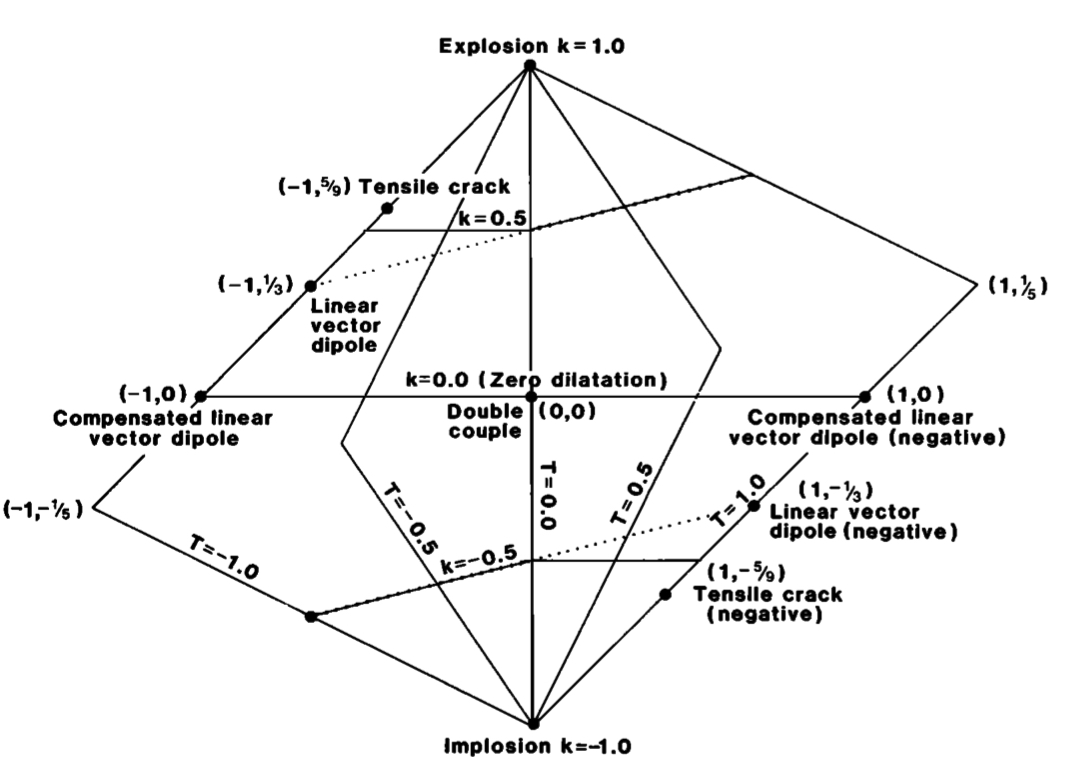
\includegraphics[width=0.9\textwidth]{source/Hudson-carton.jpg}
    \caption{Hudson图,等面积震源类型分类图}
    \label{fig:Hudson-carton}
    \note{注:虚线表示在p波辐射图中存在节点表面的区域,在该虚线外P波辐射的极性都是相同的,并且在上、下区域极性分别为正、负。
    图片引自\citep{Hudson1989}}
\end{figure}


\subsubsection{Lune 图}
Lune的源类型图在单位球体上,Hudson的源类型图等价于在单位立方体上\citep{tape2012geometric}。
球体上的图优于立方体上的图,因为它更简单,对特征值概率的假设更自然,更符合标量地震矩的欧几里得定义。
一个沙滩球是由矩张量的特征值和特征向量决定,在Lune图中特征值决定了球的大小和图案,特征向量决定了方向。
Tape将特征值的三元组$\Lambda = (\lambda_1,\lambda_2,\lambda_3)$,定义为$\lambda-space$空间,并将具有不同特征向量的沙滩球画在$\lambda-space$上对应点的位置上。
在不同位置的沙滩球可以直观地表示出矩张量之间的差异性。
当特征值$\Lambda = (\lambda_1,\lambda_2,\lambda_3)$固定时,我们得到所有的沙滩球都有固定的模式和大小,但有不同的方向(特征向量可能不同),它们之间可以通过旋转得到完全一致,如下图。
\begin{figure}[h]
    \centering
    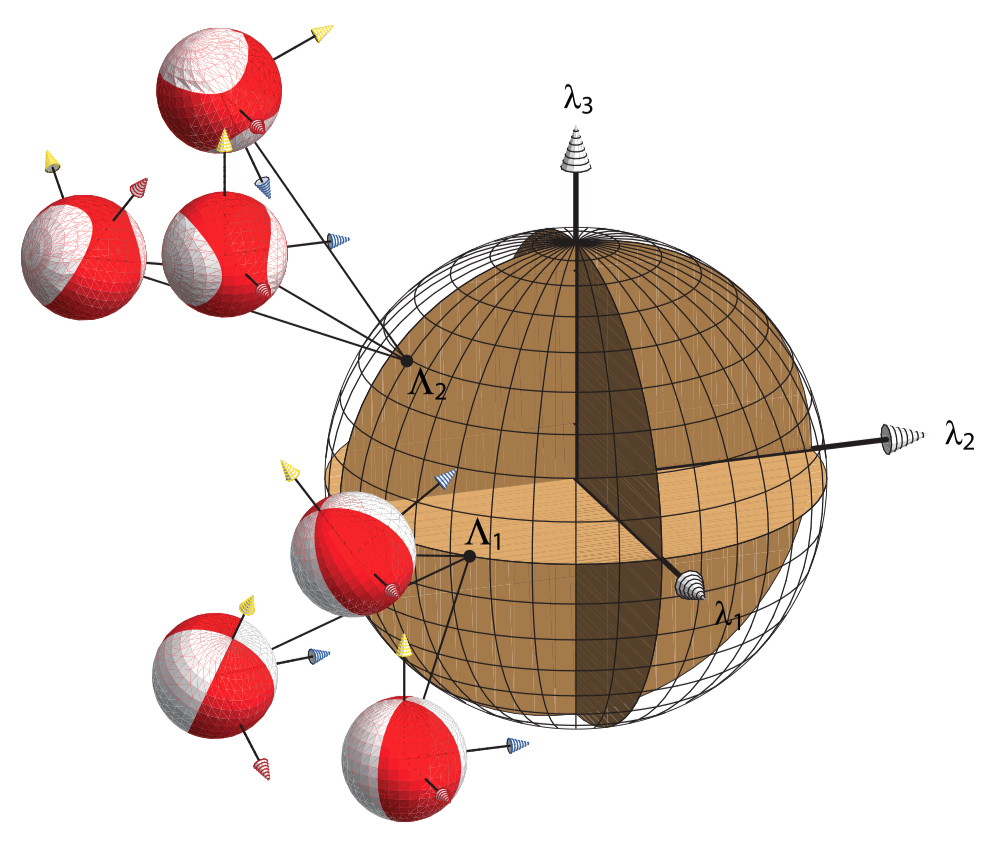
\includegraphics[width=0.9\textwidth]{source/lune-ball.jpg}
    \caption{λ-space 空间中的沙滩球}
    \label{fig:lune-ball}
    \note{注:沙滩球上的红色、蓝色和黄色箭头表示对应的特征向量。
    图片引自\citep{Tape2012}}
\end{figure}

当我们对三个特征值进行排序时,可以将所有的沙滩球转移到一个基本月球图上(fundamental lune),
该月球图上的经纬度信息与三个特征值满足下列关系:
\begin{align}
    tan \gamma = & \frac{- \lambda_1 + 2\lambda_2 - \lambda_3 }{\sqrt{3} \lambda_1 - \lambda_3}  \notag \\
    cos \beta = & \frac{\lambda_1 + \lambda_2 + \lambda_3}{\sqrt{3}  \Vert \Lambda \Vert }
\end{align}
其中$\gamma$表示Lune图上的经度,$\beta$表示Lune图上的纬度,$\Vert \Lambda \Vert = {(\lambda_1^2 + \lambda_2^2 + \lambda_3^2 )}^1/2$。
$\gamma$的范围为$[-\frac{\pi}{6},\frac{\pi}{6}]$,$\beta$的范围为$[-\frac{\pi}{2},\frac{\pi}{2}]$。
一个基本的Lune图如下所示。
\begin{figure}[h]
    \centering
    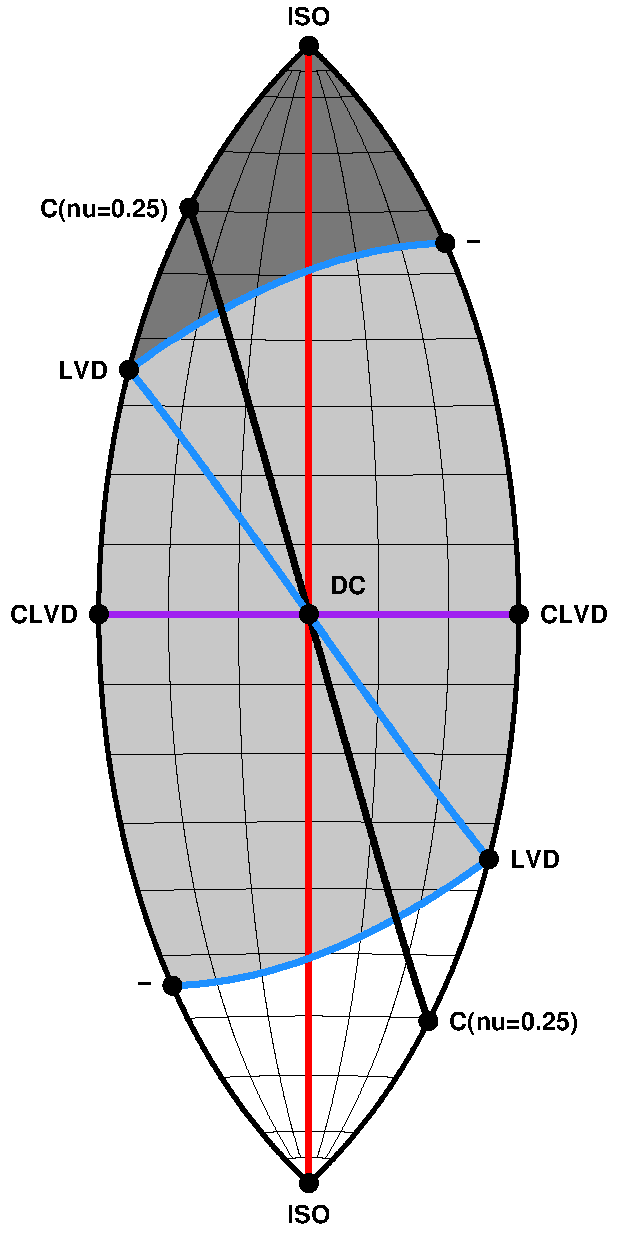
\includegraphics[width=0.4\textwidth]{source/lune-hammer-iplot-0.pdf}
    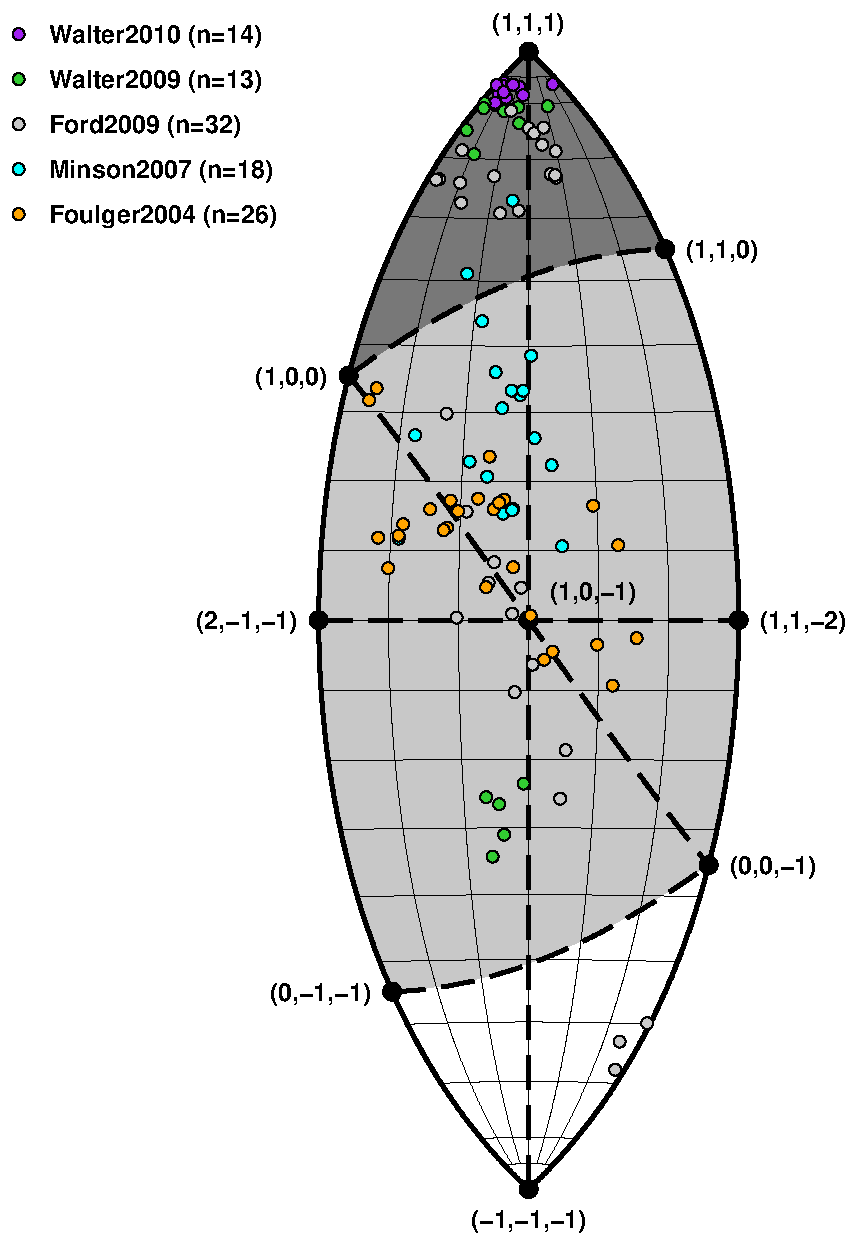
\includegraphics[width=0.55\textwidth]{source/lune-hammer-iplot-1.pdf}
    \caption{λ-space 空间中的沙滩球}
    \label{fig:lune-hammer}
    \note{注:右子图中展示了5个矩张量数据集,
    颜色分别是紫色\citep{walter2010evidence},
    蓝色\citep{walter2009moment},
    绿色\citep{minson2007seismically},
    橙色\citep{foulger2004non},
    红色\citep{ford2009identifying}。
    图片引自\href{https://sites.google.com/alaska.edu/carltape/home/research/beachball_gallery}{Carl Tape's website}。}
\end{figure}


\section{震源机制反演方法}
许多地震学与大地测量的方法可以用来确定地震震源机制。
本节主要关注地震学的方法,包括简单的测定不同相位的极性符号,测量波形的振幅和完整的波形信息等。

\subsection{地震波极性}






P波的初动极性是最常用的确定震源机制的方法,即使使用单分量地震仪低动态范围的地震仪,它包含的地震波信息最少,仅有某个相位的极性。
极性对于研究非双力偶震源非常有限,即使在沙滩球上有分布良好的观测结果,在实践中通常也很难区分双力偶模型与非双力偶模型(图~\ref{fig:p-polarity})。
因此地震学家在使用P波极性时,通常将震源模型限制为双力偶模型。
反演双力偶震源机制相当于找到两个正交的节平面,
可以通过三个独立的量(断层面走向、倾角和滑移矢量)来确定节点面。
该方法另一个局限是,只有在台站数目较充足、且台站分布较均匀的情况下,才具有较高可信度,这无疑给小地震震源机制解的确定带来困难。
除了P波的极性,有些研究也使用瑞雷面波的极性相位,Toksöz观察到内华达试验场地下核爆炸产生的Rayleigh面波的极性有时是反向的,他们从核爆破坏区释放的剪切应变来解释这一现象\citep{toksoz1972tectonic}。
\begin{figure}[h]
    \centering
    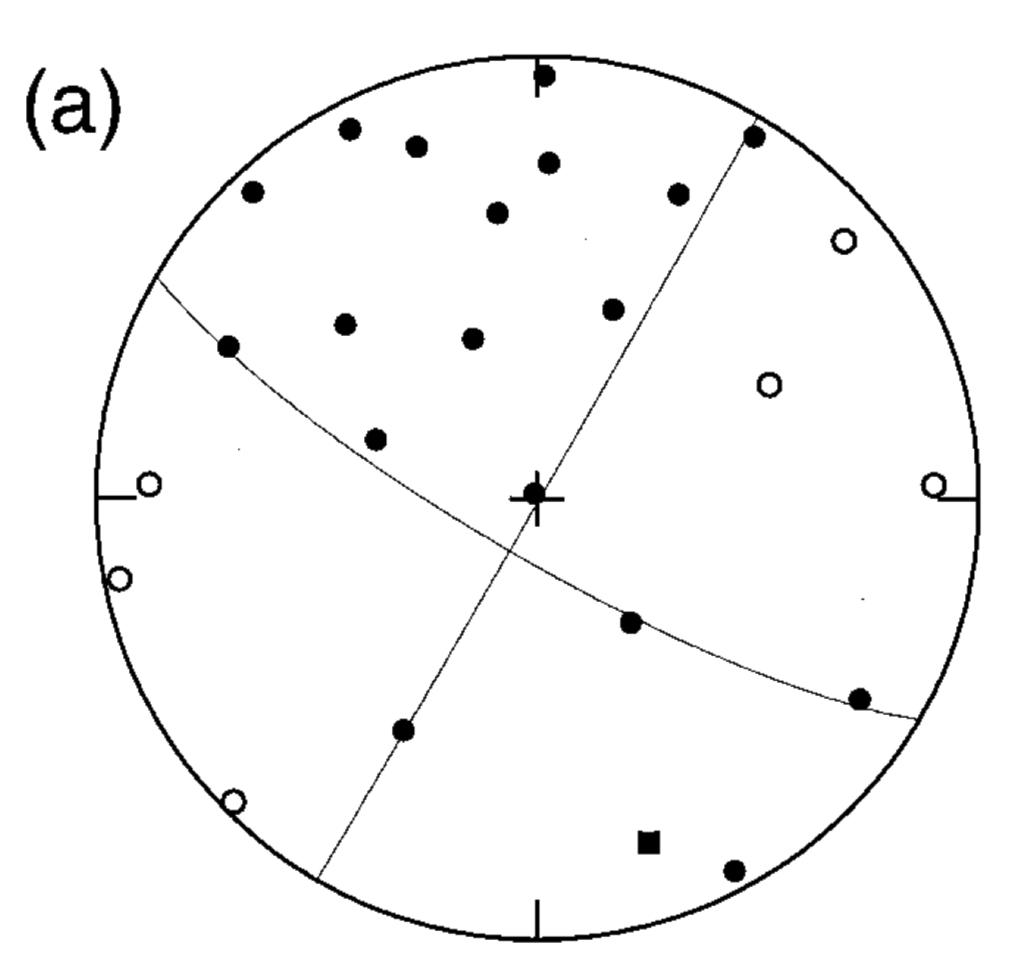
\includegraphics[width=0.45\textwidth]{source/p-polarity-a.jpg}
    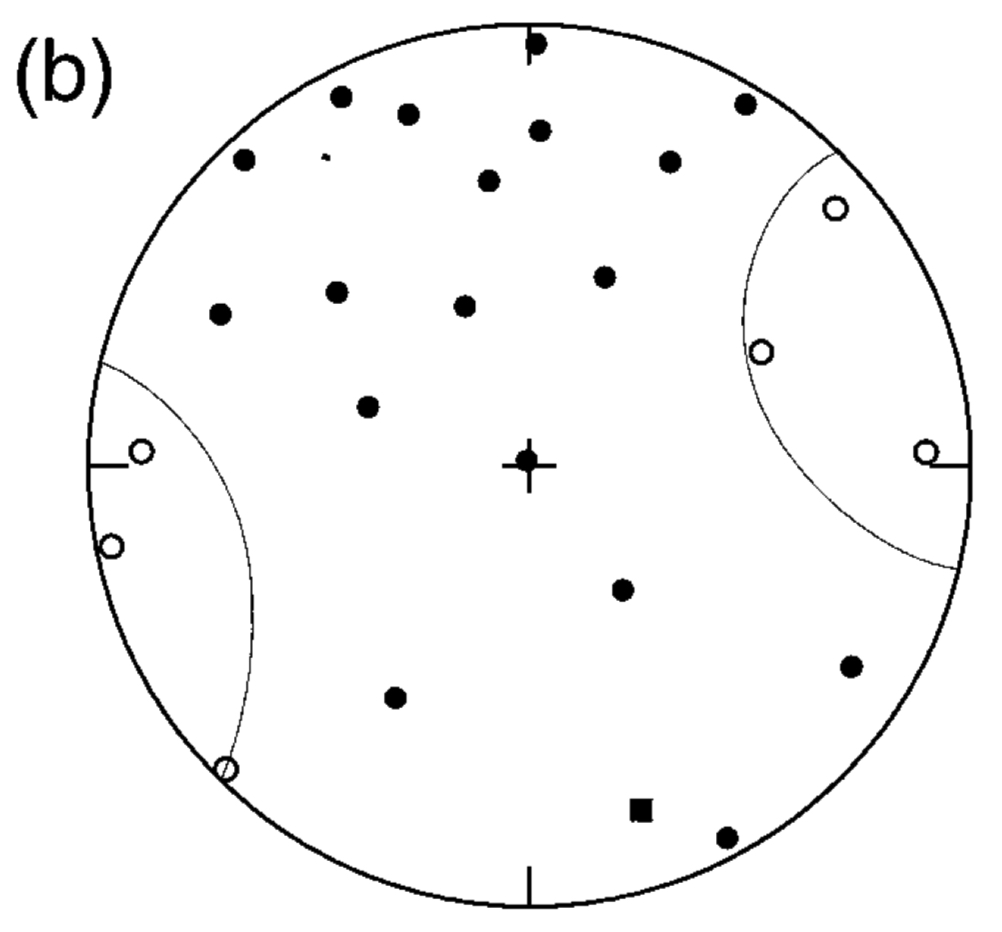
\includegraphics[width=0.45\textwidth]{source/p-polarity-b.jpg}
    \caption{P波初动极性的局限}
    \label{fig:p-polarity}
    \note{注:UTC时间1991年9月15日7时41分在冰岛亨吉尔地热地区发生的地震。
    图(a)的双力偶模型可以满足所有P波初动极性数据的要求;图(b)的矩张量震源机制通过同时反演体波极性和振幅比得到,具有较大的各向同性分量。
    图片引自\citep{julian1998non}}
\end{figure}


\subsection{地震波波振幅比}
地震波的振幅也携带着地震震源机制的信息,地震波的振幅在传播过程中会发生形状与相位上的变化,特别是速度结构非均质性引起的变化。
在利用振幅信息反演地震震源机制时,一种降低速度结构影响的方法是使用相似路径的地震波的振幅比值作为约束条件,如$P/SV$,$P/SH$,或$SH/SV$等。

图~\ref{fig:p-sv-ratio}显示了同一地震观测的$P/SH$振幅比,以及图~\ref{fig:p-polarity}所示的震源机制。
振幅比的结果表明,这次地震不是双力偶地震,它有较大的各向同性分量。
地震波振幅比相比相位初动极性,包含更多地震波的信息,进一步提高了震源参数的约束能力。
但其依旧受限于台站数量与分布。

\begin{figure}[h]
    \centering
    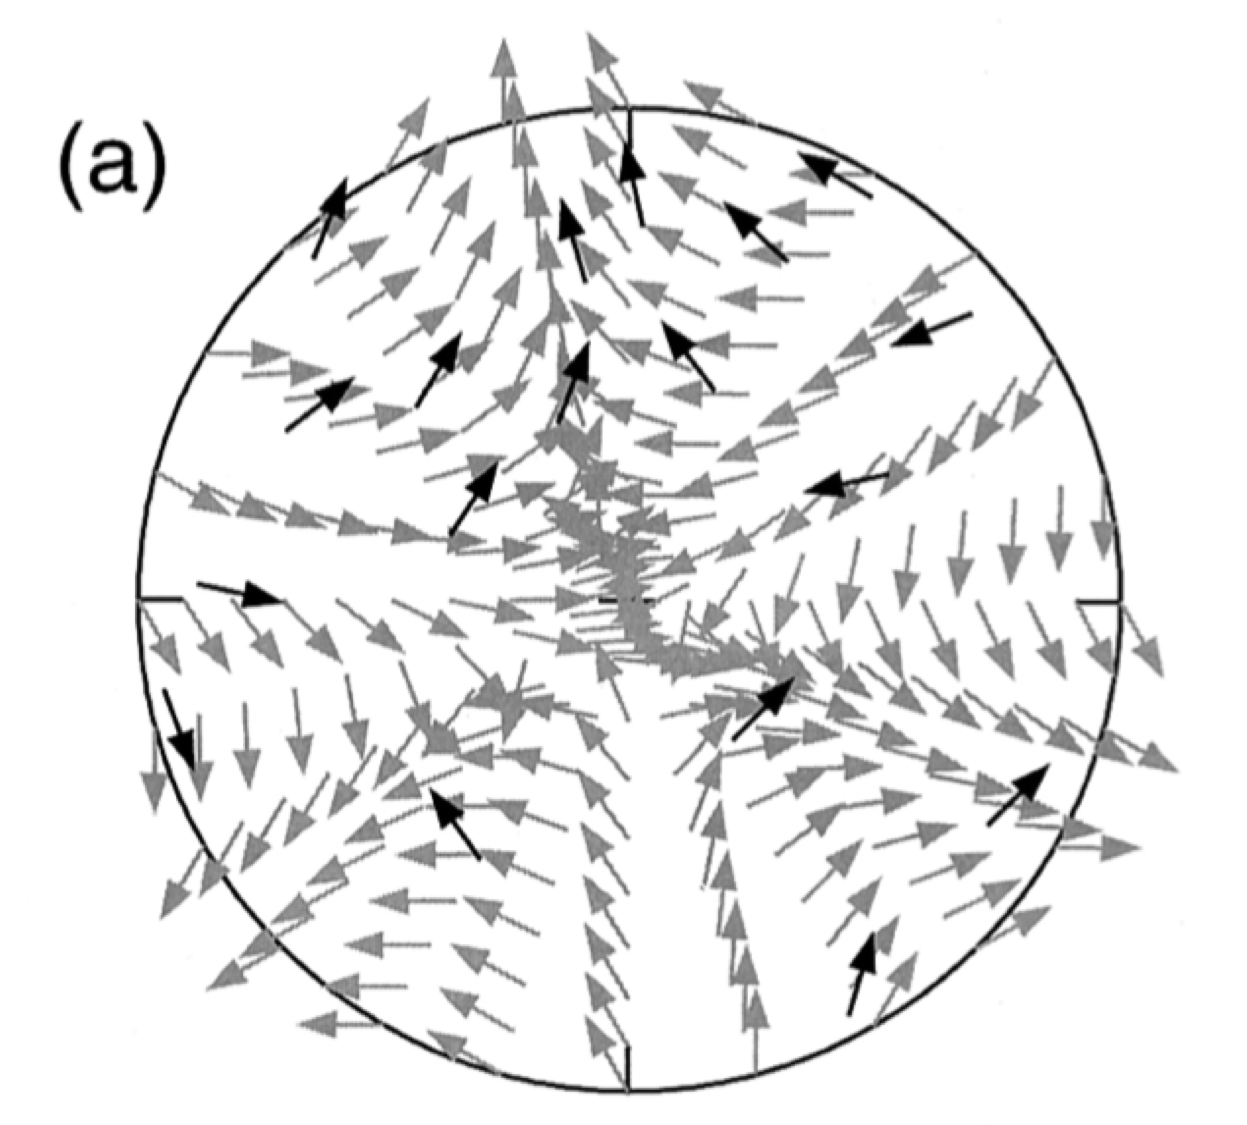
\includegraphics[width=0.45\textwidth]{source/p-sv-ratio-a.png}
    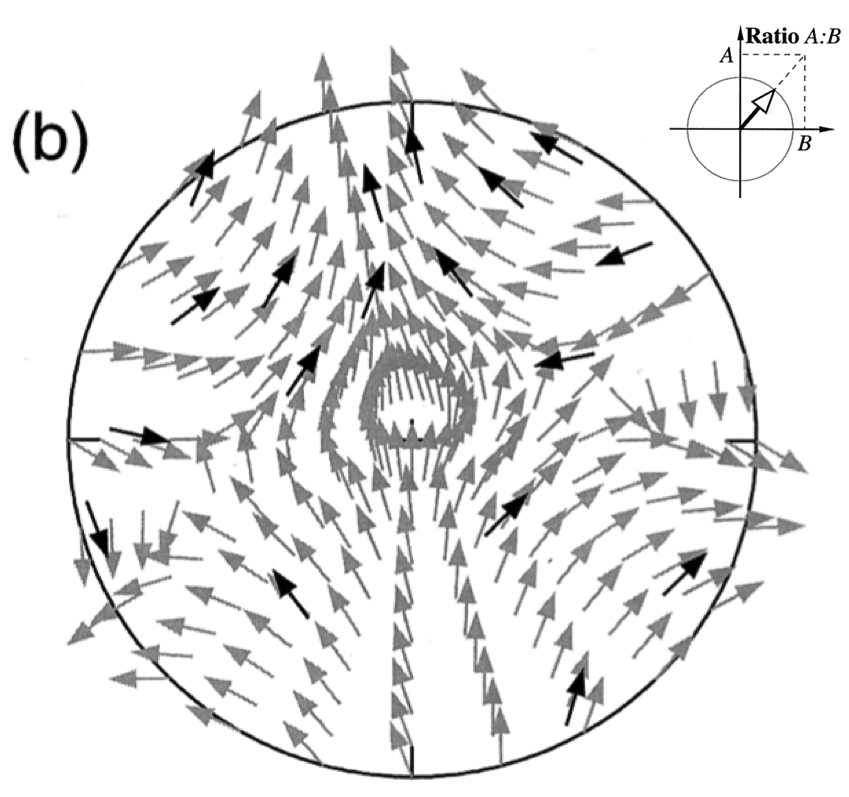
\includegraphics[width=0.45\textwidth]{source/p-sv-ratio-b.jpg}
    \caption{P波SH波振幅比}
    \label{fig:p-sv-ratio}
    \note{注:UTC时间1991年9月15日7时41分在冰岛亨吉尔地热地区发生的地震。
    理论的振幅比是黑色箭头,观测的振幅比是黑色箭头,振幅的比例都用箭头的方向表示(见插图)。
    图(a)的双力偶模型;图(b)的矩张量模型。
    图片引自\citep{julian1998non}}
\end{figure}



\subsection{地震波形反演}
近年来,随着地震观测技术不断提高,大量宽频带地震仪投入使用,利用地震波形信息进行震源机制反演成为了主流方法。
地震波形信息可以看做是一系列地震振幅信息,相当于振幅反演方法的延伸。
波形的使用,可以反演震源时间函数,但通常局限于反演问题的非线性程度与数据质量,震源时间函数通常被人为指定,并假设矩张量的所有分量都具有相同的时间函数。
波形方法本质上是振幅反演,用整个波形来进行振幅反演,比用某相位峰值反演更为精确。
波形方法最严重的限制因素是准确的格林函数,
目前详细的三维速度模型还很少存在,仅有极个别区域存在较准确的三维速度模型。
当速度模型不准确时,利用高频信息进行反演会存在严重的限制,所以大多数波形反演研究都使用长周期地震波(频率低于0.1Hz)。
对震源时间函数的简单假设,虽然会减少计算量与非线性问题,但并不适合研究未知的震源过程,如非双力偶地震,因为这些假设可能不成立。

哈佛大学和美国地质调查局(USGS)都以近乎实时的方式测定世界各地大地震的矩张量,并在地震发生后的几个小时内发布结果。
但是这些机构都将震源机制限制为只有偏量部分,不适合研究非双力偶地震的矩张量。
哈佛大学从1982年开始进行质心矩张量(CMT)的常规计算,
哈佛大学给出了矩张量的误差,但没有给出完整的协方差信息。
美国地质调查局也从1982年开始定期测定全球矩张量解,同样没有给出矩张量分量中包含的不确定性信息。

震源机制解的不确定性估计是十分重要的,因为噪声与测量误差的存在,反演结果的不确定性是必然存在的。
传统的网格搜索或者最小二乘的方法,会提供一个最优解,但我们不知道矩张量参数的后验概率空间是什么样子,所以无法评判最优解的可信性。
下面我们提出一种利用贝叶斯蒙特卡洛进行波形反演的方法,它能够确定地震震源机制中存在的不确定性信息。



\section{MCMTpy原理与框架}

在本节我们将会展示MCMTpy程序包的基本原理与使用流程,主要包含贝叶斯推理,格林函数的计算,
误差函数的定义,与程序包的特点。


\subsection{原理方法}

\subsubsection{贝叶斯推理}

通常一个地球物理反问题包含三部分:
观测参数$d_{obs}$(也称观测数据);
模型参数的先验信息$\pi_{prior}(m)$和观测数据的先验信息$\pi_{prior}(d_{obs})$;
以及观测参数与模型参数的物理数学联系,也称之为条件概率密度函数$\pi_{like}(d_{obs}|m)$(Revelo Obando, 2018).
贝叶斯推理提供了一种量化地球物理反演问题中不确定性的方法\citep{Zhao2019}。
贝叶斯反问题的解通常表示为模型后验概率密度(posterior probability density,简写PPD),
即$\pi_{post}(m|d_{obs})$,其数学表达为:
\begin{equation}
    \pi_{post}(m|d_{obs})=k \pi_{prior}(m) \pi_{like}(d_{obs}|m)
\end{equation}
其中$d_{obs}$是观测数据向量,$k$是贝叶斯理论中的正则化参数,$m$是需要评估的模型参数向量,
在MCMTpy的双力偶模型中被写成:
\begin{equation}
    m=(M_w,strike,dip,rake,lat,lon,depth,T_0)
\end{equation}
矩张量模型中被写成:
\begin{equation}
    m=(M_0,M_{xx},M_{xy},M_{xz},M_{yy},M_{yz},M_{zz},lat,lon,depth,T_0)
\end{equation}
其中$M_w$是矩震级,$M_0$是标量地震矩,$M_{xx},M_{xy},M_{xz},M_{yy},M_{yz},M_{zz}$是
震源矩张量的6个正则化分量,$T_0$是地震事件发震时刻的偏移量。

我们的目标是通过给定先验模型参数$\pi_{prior}(m)$,去评估后验概率密度PDD $\pi_{post}(m|d_{obs})$。
先验信息反映了在我们获得数据信息之前,对模型参数的信息了解情况\citep{Shen2013}。
在本研究中先验信息包含:矩震级、震源位置与震源机制。
通常先验信息由人为经验或先前研究结果决定,当没有明确的先验信息时,我们使用均匀分布表示先验信息:
\begin{equation}
    \pi_{prior}(m) =
    \begin{cases}
      \frac{1}{b-a} & \text{for } a \le m \le b, \\
      0             & \text{otherwise}.
    \end{cases}
\end{equation}
其中$a$和$b$分别是模型参数的搜索边界。假设模型参数$m$的噪声可以表示成多元高斯函数分布,那么
\begin{equation}
    \pi_{post}(m|d_{obs}) \propto \pi_{like}(d_{obs}|m) = exp \biggl\{ -\frac{1}{2} S(m) \biggr\},
\end{equation}
其中$S(m)$是误差函数,它可以被定义为:
\begin{equation}
    S(m) = \bigl( d_{obs}-f(m) \bigr) ^T {C_k}^{-1} \bigl( d_{obs}-f(m) \bigr) 
\end{equation}
其中 $f(m)$是根据模型参数$m$预测的数据。
$C_k$是数据集的残差协方差矩阵,通常该协方差是未知的,需要在反演采样前由人为经验给出。
要注意协方差$C_k$的选取对贝叶斯评估结果有较大的影响\citep{Duputel2012,Vasyura-Bathke2020}。

基于马尔科夫链的蒙特卡洛方法通常会对模型参数空间进行随机采样,从而得到后验概率分布。
是否接受某次随机采样结果,即从模型$m_k$到新模型$m_{k+1}$,取决于转换核函数$\beta(m_k,m_{k+1})$,
根据Metropolis-Hasting (M-H)准则\citep{Metropolis1953},其被定义为:
\begin{equation}
    \beta(m_k,m_{k+1}) = min \biggl\{ \frac{\pi_{post}(m_{k+1}|d_{obs})} {\pi_{post}(m_{k}|d_{obs})}, 1   \biggr\},
\end{equation}

如果误差函数$S(m_{k+1})$比$S(m_{k})$小,那么我们会接受新模型$m_{k+1}$。
如果新模型$m_{k+1}$产生了一个较大的误差,那么我们会以“一定概率”接受新模型,
而不是直接拒绝新模型,这样做可以避免陷入局部极小值。“一定概率”即是转换核函数$\beta(m_k,m_{k+1})$。
经过大量采样,马尔科夫链会达到一个概率稳定的状态,模型参数的不确定性可以从后验概率PDD中量化。


\subsubsection{格林函数与合成地震记录}

为了计算预测数据向量$f(m)$,我们需要计算整个研究区域的格林函数。
MCMTpy使用Pyfk程序包(一个Python版本的频率波束合成地震记录方法)(Zhu and Rivera, 2002)来计算一维地球模型。
双力偶模型下的合成地震记录可以表示为:
\begin{equation}
    V(t)=M_0 \sum_{i=1}^3 A_i(\phi - \theta, \delta, \lambda ) G_i(t),
\end{equation}
其中$i=1,2,3$分别对应三个基本形式的断层,即断层倾角$90°$的走滑断层(vertical strike-slip),断层倾角$90°$的倾滑断层(vertical dip-slip),和断层倾角$45°$的倾滑断层 (45° dip slip)。
$\theta$,$\lambda$和$\delta$分别表示震源与台站之间方位角与断层走向、滑动角与倾角之间的差异角度。
$\phi$表示台站方位角,$G_i(t)$是格林函数,$A_i$是震源辐射系数。
$M_0$是地震矩,单位为dyne($10^7 dyne = 1N \cdot m$),
其与地震矩震级 $M_w$\citep{Kanamori1993}的关系为:
\begin{equation}
    M_w = \frac{2}{3} log_{10}(M_0) - 10.7.
\end{equation}
对于矩张量模型下的合成地震记录可以表示为:
\begin{equation}
    V(t) = M_{ij} G_{ij}(t),
\end{equation}
其中$M_{ij}$是6个独立的矩张量分量,$G_{ij}$是其对应的格林函数。


\subsubsection{误差函数}

MCMTpy程序同时使用相位到时信息与波形信息,对震源模型参数进行后验概率采样。
其误差函数$S(m)$定义为:
\begin{equation}
    S(m)=
    \begin{cases}
        S_{time}(m)   &  k \le K_n  \\
        S_{wave}(m)   &  k > K_n
    \end{cases}
\end{equation}
其中$S_{time}(m)$和$S_{wave}(m)$分别表示相位到时信息与波形拟合的残差。
$k$是采样总数;参数$K_n$把误差函数$S(m)$分为两个阶段。
在第一个阶段,我们使用相位到时误差函数(作为一个辅助函数),搜索出一个相对准确的震中位置。
然后在第二个阶段,我们使用波形拟合函数(作为一个核心采样函数),同时对地震位置(矩中心位置)和震源机制进行采样,
并评估位置与震源机制的不确定性。

相位到时误差函数 $S_{time}$ 同时使用 P波与S波到时,定义为:
\begin{equation}
    S_{time}(m) = \frac{1}{N} \sum_{i=1}^N \frac{{[T_i(m) - {T_i}^{obs} - T_0]}^2} {{\sigma_i}^2}
\end{equation}
其中$T_0$是地震事件发震时刻的偏移值,通常设置其初始值为0,
${T_i}^{obs}$是第$i$个台站的相位到时,总共有$N$个台站。
$T_i(m)$是根据模型$m$得到的相位到时预测值,其使用$ObsPy-TauP$到时计算工具获得\citep{Crotwell1999,Beyreuther2010}。
$\sigma_i$表示相位到时的不确定性值。

$S_{wave}$的残差被定义为观测波形与理论合成波形的差值,表示为:
\begin{equation}
    e = \frac{1}{npts}  {\Vert V^{obs}(t) - M_0 V(t-\delta t) \Vert|}^2 
\end{equation}
其中$V^{obs}$是观测波形,$V$是单位矩震级时的理论合成波形。
$\delta t$是时间偏移量,其是为了考虑速度模型的不准确性引入的。
$npts$是$V^{obs}$与$V$波形对应的采样点个数。
波形分别包含P波、S波和面波的垂直、径向和切向三个部分。
总的误差函数$S_{waveform}$定义为所有台站误差函数的叠加:
\begin{multline}
    S_{waveform} = \frac{1}{N} \sum_{i=1}^N \frac{{w_i}^{station}}{{\tau_i}^2} \biggl\{  
         {w_i}^p {(\frac{r_i}{r_0})}^{ps_p} ({e_i}^{p_z}+{e_i}^{p_r}+{e_i}^{p_t}) \\
        + {w_i}^s {(\frac{r_i}{r_0})}^{ps_s} ({e_i}^{s_z}+{e_i}^{s_r}+{e_i}^{s_t}) 
        + {w_i}^{surf} {(\frac{r_i}{r_0})}^{ps_{surf}} ({e_i}^{surf_z}+{e_i}^{surf_r}+{e_i}^{surf_t}) 
        \biggr\} 
    \label{equ:misfit-function-2}
\end{multline}
其中$r_i$表示台站$i$与地震事件之间的距离;$r_0$表示所有台站里最小的震中距。
$ps$是标量因子,用于平衡体波与面波不同几何扩散系数对波形振幅造成的影响。
参考CAP的方法\citep{Zhao1994,Zhu1996},
对于体波,我们设置 $ps = 2$,对于面波,我们设置$ps = 1$。
${w_i}^{station}$是台站$i$的权重因子。
${w_i}^p$、${w_i}^s$和${w_i}^{surf}$分别是P波、S波和面波的权重因子,通常设置其范围在0到1之间,
0表示不使用相关相位。
$\tau_i$表示波形拟合的不确定性。
我们使用互相关函数衡量观测波形与理论合成波形之前的匹配性:
\begin{equation}
    C(t) = \frac{\int_{t_1}^{t_2} V(\tau) V^{obs}(t+\tau) d\tau}
    {{ \left[ \int_{t_1}^{t_2} V^2(\tau) d\tau \int_{t_1}^{t_2} {V^{obs}}^2(\tau) d\tau \right] }^{1/2}    }
\end{equation}
其中$C(t)$的最大值定义为互相关系数。
$t_1$和$t_2$分别是互相关运算的开始与结束时刻。
当$C(t)$取最大值时对应的时间偏移定义为公式(2.13)的$\delta t$。

需要注意的是直接评估数据协方差矩阵$C_k$公式(2.6)的非对角元素是非常困难的。
我们假设相位到时数据与波形拟合数据的误差是独立分布的,那么协方差矩阵就可以表示为
仅含对角元素${\sigma_i}^2$和${\tau_i}^2$。
这样的处理方法也被普遍使用于联合反演中\citep{Shen2013,Fang2016}。



\subsection{反演流程}

为了更好比较MCMTpy与传统方法的工作流程,我们展示流程对比图(图~\ref{fig:workflow})。
传统的反演方法通常包含两步:第一步先反演震源位置,通常使用加权最小二乘方法去优化相位到时目标函数\citep{klein1989user};
然后第二步使用第一步获得地震位置信息,进一步反演震源机制,通常使用网格搜索的反演方法\citep{Zhu2016}。
因为第二步需要使用第一步反演的结果,这会导致最终的反演结果包含两步中的累积误差。

\begin{figure}[h]
    \centering
    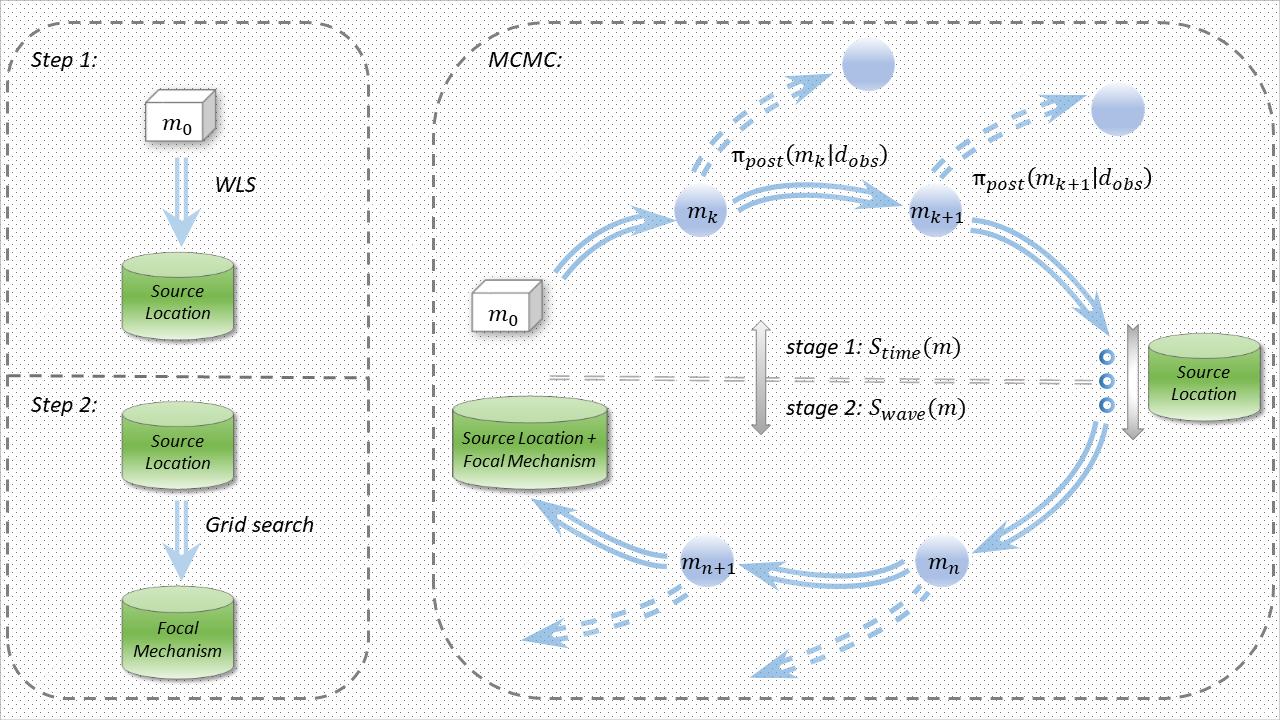
\includegraphics[width=0.9\textwidth]{source/workflow.png}
    \caption{MCMTpy与传统两步法反演流程对比}
    \label{fig:workflow}
    % \note{注:图注的内容不宜放到图题中。}
\end{figure}

MCMTpy方法把地震定位与震源机制反演两个步骤,合并成一个反演过程。
传统上模型参数的后验概率密度(PDD)通常基于M-H准则,使用马尔科夫蒙特卡洛的采样方法获得。
与传统方法不一样的是,MCMTpy会在不同采样时期采用不同的误差函数进行采样。
在第一个时期,MCMTpy使用相位到时误差函数$S_{time}$约束地震位置。
然后在第二个时期,马尔科夫链会使用第一个时期最新的地震采样位置或者最大概率(MAP)位置,进行下一步采样,
此时会同时对震源位置与震源机制进行采样,这会进一步约束地震位置并减小波形拟合误差。
然而传统的两步法只能使用固定的地震位置去反演震源机制,忽略了地震位置的误差的存在。

在采样的最开始的“热身”阶段,MCMTpy会使用下述公式粗略的估计地震标量矩的大小:
\begin{equation}
    M_0 = \frac{1}{N} \sum_{i=1}^N \frac{\Vert {V_i}^{obs} \Vert}{\Vert V_i \Vert}
\end{equation}
新的模型通常上一个模型的状态生成:
\begin{equation}
    m_{k+1} = m_k + N_g(0,\sigma(k))
\end{equation}
其中$N_g(0,\sigma)$是均值为0,标准差为$\sigma$的高斯分布;$\sigma$通常也被称为搜索步长。
关于具体的采样算法如下(算法~\ref{algo:MCMTpy})所示:

\begin{algorithm}[h]
    \SetAlgoLined
  
    Choose initial $m_0$,$S(m_0)$\;
    Compute $\pi_{post}(m|d_{obs})$\;
    \For{$k = 0,\dots,N-1$}{
        \eIf{$k<N_k$}{
            Define $S(m)=S_{time}(m)$\;
        }{
            \If{$k<N_k+M_{mag}$}{
                Estimate $M_0$ with formula XX\;
        }
        Define $S(m)=S_{time}(m)$\;
        }
        Draw sample $y$ with random walk with formula 17\;
        Compute $\pi_{post}(y|d_{obs})$\;
        Compute $\beta(m_k,m_{k+1}) = min \biggl\{ \frac{\pi_{post}(m_{k+1}|d_{obs})} {\pi_{post}(m_{k}|d_{obs})}, 1   \biggr\}$ \;
        Draw random number $u \sim u([0,1])$\;
        \eIf{$u<\beta(m_k,m_{k+1})$}{
            Accept: set $m_{k+1}=y$\;
        }{
            Reject: set $m_{k+1}=m_k$\;
        }
    }
    \caption{MCMTpy algorithm to sample proposal distribution $\pi_{post}(m|d_{obs})$}
    \label{algo:MCMTpy}
\end{algorithm}



\subsection{程序功能}

伴随着科学计算的快速发展,Python编程语言在地震学的研究中越来越受欢迎。
MCMTpy利用Python编写,是一个新的震源参数反演框架,它与现在流程的地震学工具紧密结合,
例如ObsPy\citep{Beyreuther2010},和MPI4py\citep{Dalcin2011}和ASDF\citep{Krischer2016}。
MCMTpy目前提供了计算一维格林函数的接口,并且支持MPI同时使用多条马尔科夫链并行采样。
此外,它具有灵活的参数设置方法,每个台站独立的滤波范围、相位与台站的权重等都可以在配置文件(JavaScript Object Notation format;例如(图~\ref{fig:flowchart})的sample.json文件)中设置。
图~\ref{fig:flowchart}是一个项目工作区示例。MCMTpy的主要功能包括:
\begin{enumerate}
\item 基于双力偶模型的马尔科夫蒙特卡洛采样与网格搜索的震源参数反演。
\item 基于矩张量模型的马尔科夫蒙特卡洛采样的震源参数反演。
\item 震源参数计算与转换,例如矩张量的分解、Hudson图\citep{Hudson1989}和Lune图\citep{Tape2012}。
\end{enumerate}
在下面两节中,我们将介绍MCMTpy方法在两次地震中的应用,分别是2021年中国云南漾濞地震反演与2008年美国Mt. Carmel地震反演。

\begin{figure}[p]
    \centering
    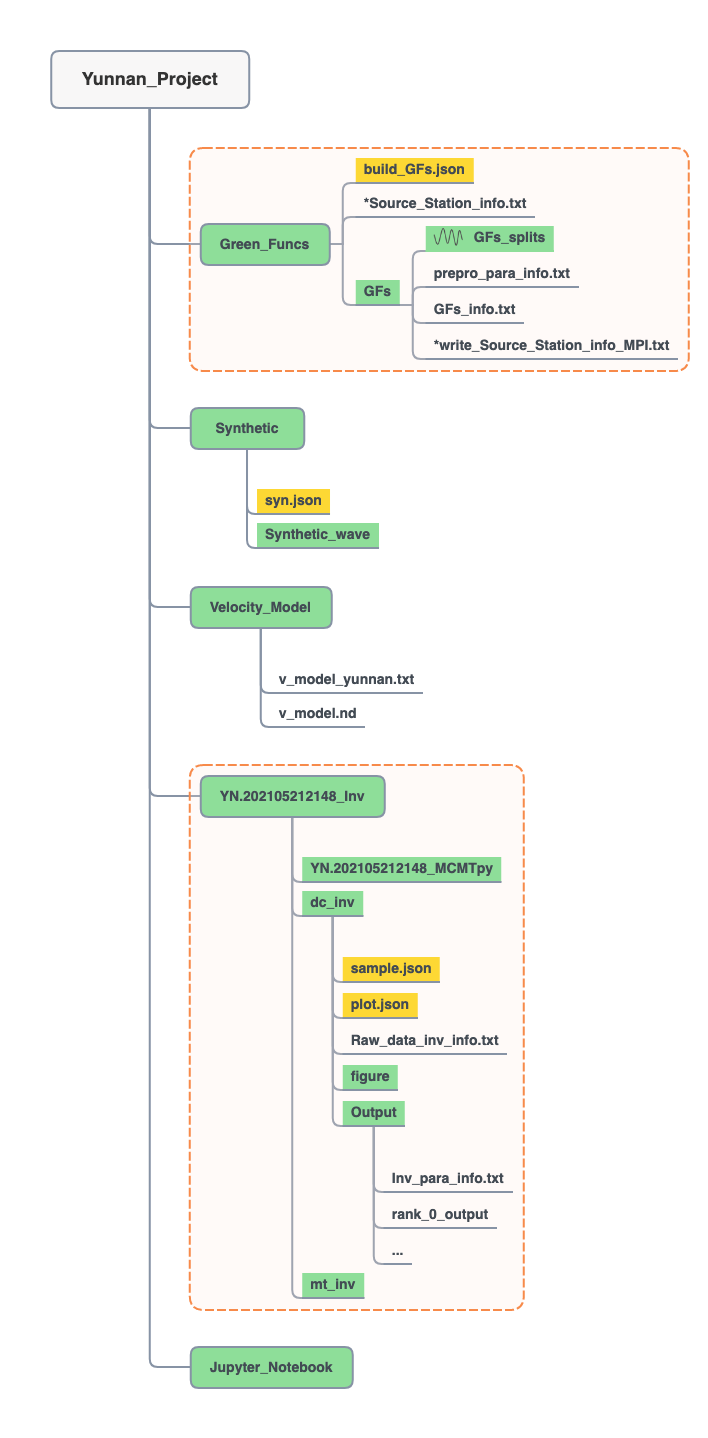
\includegraphics[width=0.6\textwidth]{source/flowchart.png}
    \caption{MCMTpy反演项目目录结构}
    \label{fig:flowchart}
    \note{ 注:"Yunnan\_project"是项目的名称;黄色背景表示配置文件"*.json";一个项目通常包含以下5个步骤:\\
    a. 在文件夹"Velocity\_Model"提供速度模型。\\
    b. 在"Green\_Funcs"文件夹下设置格林函数库配置文件"build\_GFs.json",然后计算格林函数。\\
    c. 在"Synthetic"文件夹下进行合成数据测试,用来检测格林函数库的正确性。\\
    d. 进行反演:准备ASDF格式的观测数据;设置采样配置文件"sample.json",进行对应的双力偶与矩张量的采样;"Output"文件夹包含所有的采样结果;"figure"包含所有结果的可视化文件。\\
    e. 在"Jupyer\_Notebook"文件夹下进行各类震源转换与后验概率的不确定性可视化。}
\end{figure}


\section{2021年中国云南漾濞地震反演}
在2021年5月21号,漾濞地震发生在中国云南省内,其位于中国的西南方(图~\ref{fig:map-yangbi})。
根据中国地震台网中心(CENC)的地震目录报告,漾濞地震的震中位置是纬度25.70°、经度99.88°、深度$10km$,GMT时间为13:48:35,面波震级为$M_s 6.4$。
因为发震位置周围拥有大量的永久型和移动型地震观测仪器,我们获得了清晰的地震波形数据。
我们使用中国西南的公共速度模型Community Velocity Model V.1.0 of Southwest China\citep{Liu2021},并将三维速度模型进行数值平均,变成一维速度模型。
我们首先计算格林函数库,其最大震中距为$800 km$。
我们从中国台网数据中心\citep{Zheng2009}获取了三分量宽频带的地震波形数据。
我们挑选震中距在7°以内的台站,台站分布见图~\ref{fig:map-yangbi}。
在剔出限幅数据和去除仪器响应后,我们将地震记录转换为速度记录。
在接下面的两节,我们将介绍双力偶与矩张量反演结果。


\begin{figure}[h]
    \centering
    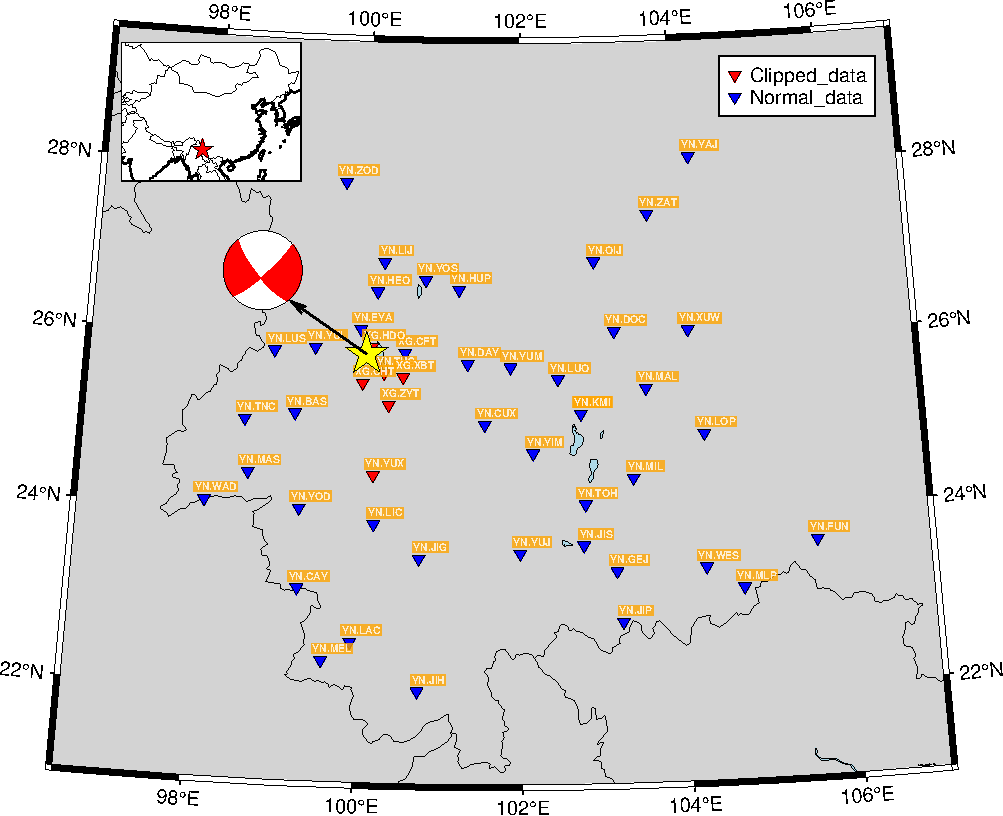
\includegraphics[width=0.9\textwidth]{source/map-yangbi.pdf}
    \caption{漾濞地震台站分布}
    \label{fig:map-yangbi}
    \note{注:左上方子图的红色五角星显示研究区域,6个红色三角形表示振幅受限的台站。}
\end{figure}

\subsection{双力偶反演}

我们选取CAP方法的反演结果(strike 135°,dip 75°,slip -168°)最为初始模型,进行双力偶模型采样,
初始模型的影响将会在下节进行讨论。
震源时间函数的持续通时间过下面公式进行估计,约为5.9s,与Scaling Law\citep{Somerville1999}准则一致:
\begin{equation}
    T_{duration} = 10^{\frac{M_w-5}{2}}+0.5
    \label{equ:duration-time}
\end{equation}
我们将地震波形数据分为$Pnl$波和面波部分。
因为S波的到时与面波的到时接近,所以S波没有参与反演。
为了最大程度利用地震的高频信号,在震中距小于100km的区域,我们使用Butterworth滤波器,
对P波进行0.01 - 0.2Hz滤波,对面波进行0.02 - 0.1Hz滤波;
在震中距较大的区域,为了抑制地壳介质三维小尺度的复杂性影响,我们对P波进行0.01 - 0.1 Hz滤波,对面波进行0.02 - 0.1Hz滤波。
观测数据与理论合成数据都被降采样到每秒5个采样点。
与上面操作对应的是,在震中距小于100km的区域,我们设置P波的拟合窗口为P波到时的前10秒与后15秒,
设置面波的拟合窗口为面波到时的前10秒与后35秒;
在震中距较大的区域,我们设置P波的拟合窗口为P波到时的前10秒与后25秒,
设置面波的拟合窗口为面波到时的前10秒与后45秒。
所有的相位与台站的权重因子都设置为1。
为了避免因为cycle skipping现象陷入局部极小值,我们严格设置了滑动窗口在相应地震记录半个波长内。
在漾濞地震中,我们估计相位到时的不确定性为0.2秒,波形的不确定性为0.09$cm/s$,我们设置参数$K_n$等于2000。
具体的滤波参数与拟合时间窗参数会随台站的不同有细微差异。
我们使用单条马尔科夫链进行20000次采样,大约需要14个小时的时间,运行系统为CentOS Linux system (2.30 GHz Intel Xeon Gold 5218 CPU)。

采样过程的归一化误差曲线见图~\ref{fig:misfit-yangbi-dc}。
我们可以看到在相位到时误差曲线$S_{time}$中,大约经过500次采样,误差就已经达到一个较低的值了,
这表明马尔科夫链经过短暂的burn-in状态搜索到typical set(特征集)并可能进行目标后验分布的采样。
同样的在波形误差曲线$S_{wave}$中,大约经过2000次采样,采样器就可能在目标后验分布附近进行采样。
图~\ref{fig:waveform-yangbi-dc}展示了波形拟合结果,图~\ref{fig:hist-yangbi-dc}展示了震源参数的后验概率的1-D与边缘后验概率的2-D分布,并显示了最优的采样结果。
我们计算了震源参数的后验分布均值与方差,见图~\ref{fig:hist-yangbi-dc}。
为了评估不同模型参数之间的trade-off,我们计算了归一化的后验分布协方差(图~\ref{fig:hist-yangbi-dc}),其中归一化的后验协方差定义为:
\begin{equation}
    Cov_0(m_i,m_j) = \frac {Cov(m_i,m_j)} {\sigma_i \sigma_j}
\end{equation}
其中$\sigma_i$表示模型参数$m_i$的后验分布标准差。
当协方差不再随着采样显著地改变时,意味着采样器对后验概率达到了一个较均衡的采样状态,如图~\ref{fig:accept-ratio}。

\begin{figure}[h]
    \centering
    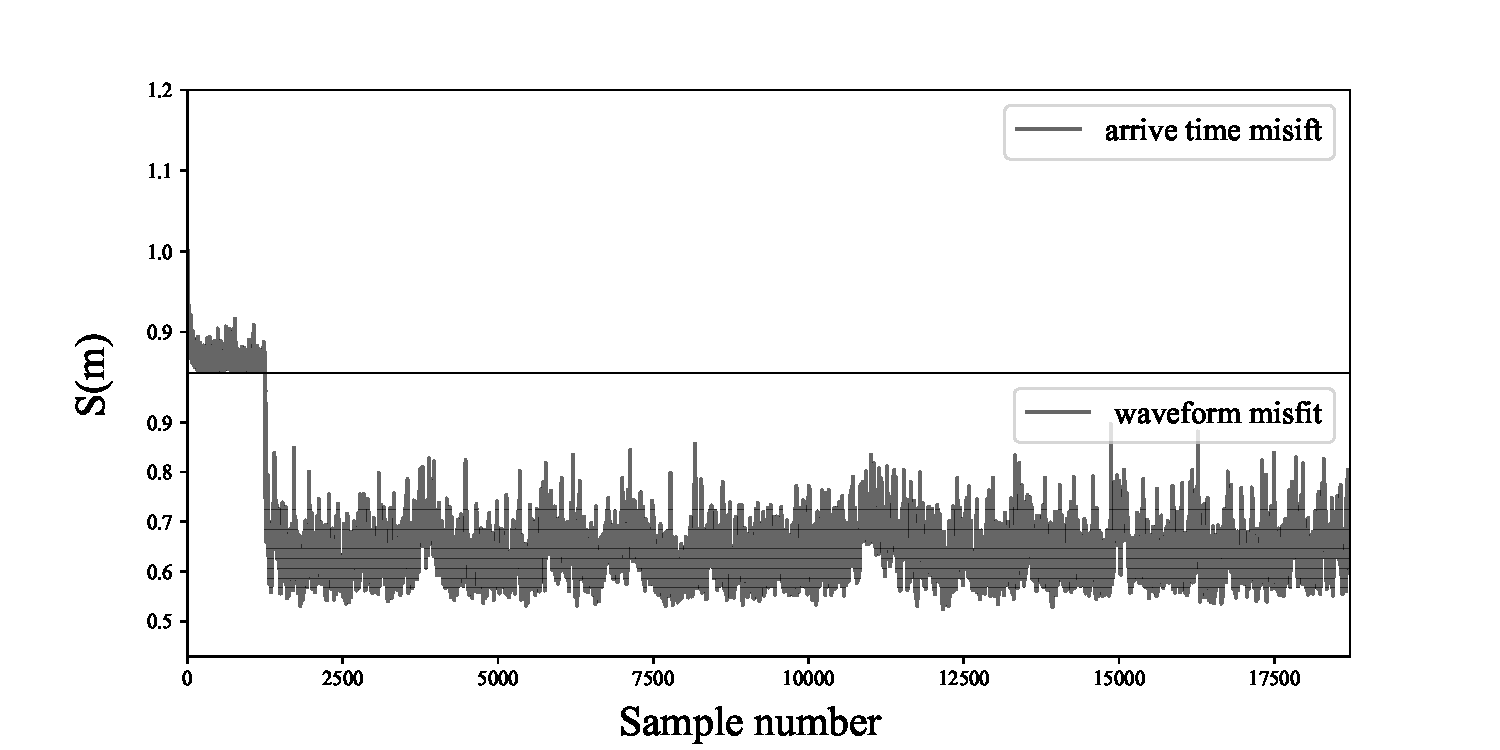
\includegraphics[width=0.9\textwidth]{source/misfit-yangbi-dc.pdf}
    \caption{漾濞地震双力偶模型反演的误差函数}
    \label{fig:misfit-yangbi-dc}
    \note{注:两个阶段的误差函数都经过归一化处理。}
\end{figure}

\begin{figure}[h]
    \centering
    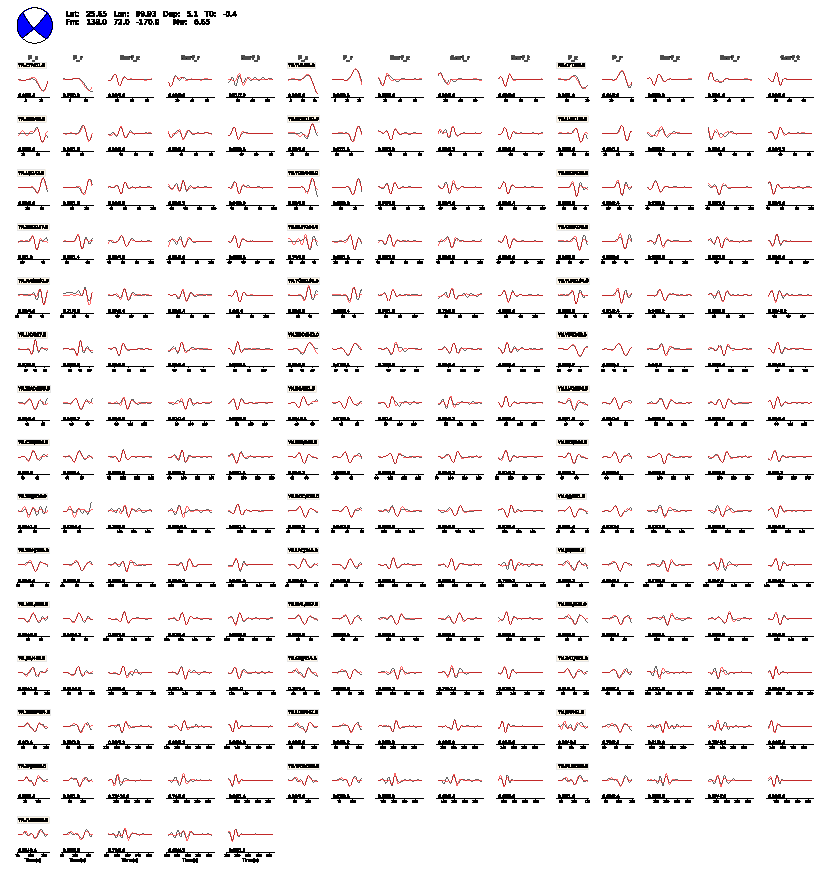
\includegraphics[width=0.9\textwidth]{source/waveform-yangbi-dc.pdf}
    \caption{漾濞地震双力偶模型反演的波形拟合}
    \label{fig:waveform-yangbi-dc}
    \note{注:观测的地震波形用灰色线表示,合成的理论波形用红线表示;
    相关系数与时间偏移量在每个子图的左下方表示;
    每个台站的标注都由台网名称、台站名称和震中距组成;
    图中P\_z和P\_r分别表示P波的Z和R分量;
    Surf\_z、Surf\_r、Surf\_t分别表示面波的Z、R和T分量。}
\end{figure}

\begin{figure}[h]
    \centering
    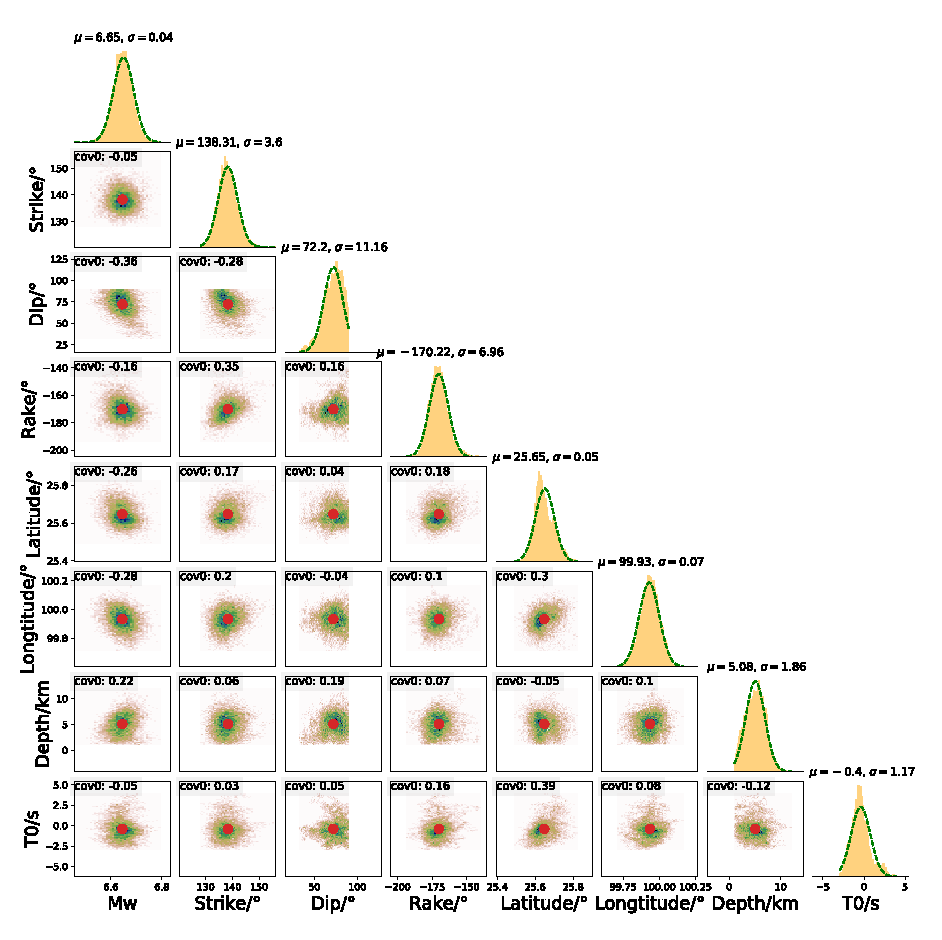
\includegraphics[width=0.9\textwidth]{source/hist-yangbi-dc.pdf}
    \caption{漾濞地震双力偶模型反演的后验概率分布}
    \label{fig:hist-yangbi-dc}
    \note{注:$\mu$和$\sigma$分别表示一维直方图的均值与标准差;
    绿色虚线表示最佳的高斯拟合分布;
    红色点表示MAP解;
    后验分布的协方差系数显示在对应子图的左上方。}
\end{figure}

\begin{figure}[h]
    \centering
    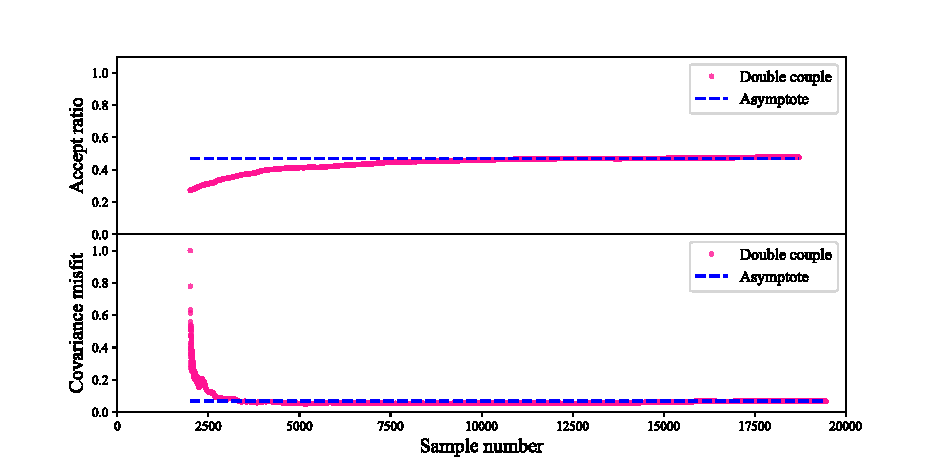
\includegraphics[width=0.9\textwidth]{source/accept-ratio.pdf}
    \caption{漾濞地震双力偶模型反演的接受率与协方差曲线}
    \label{fig:accept-ratio}
    \note{注:蓝色点线表示接受率与协方差的渐近线。}
\end{figure}

不同机构提供了不同的震源参数反演结果,见表~\ref{tab:yangbi-1}。不同机构给出的地震震级差异较大,我们的反演结果显示了最大的震级($6.65M_w$);
一个可能的原因是我们使用的部分台站靠近盆地,盆地导致了地震波的方法,而Global CMT和USGS机构
使用来自全球地震台网的长周期地震波,其不会受到这些影响。
我们反演结果的走向角,倾角和滑动角非常接近USGS W-phase和CAP\citep{Long2021}的结果,
其中CAP方法使用了9个震中距在200km以内的台站,并且台站具有较好的台站分布。
Global CMT和USGS机构给出的地震深度超过15km;作为对比,我们的结果显示一个较浅的地震深度只有5km,
该结果与CAP的结果相一致\citep{Long2021}。

\begin{table}[h]
  \centering
  \caption{Source Parameters in 2021 Yangbi Earthquake of Different Agencies}
  \label{tab:yangbi-1}
%   \begin{tabular}{c|cccp{6em}p{3em}c}
    \centering%把表居中
    \begin{tabular}{m{2cm}<{\centering}m{1.5cm}<{\centering}m{2cm}<{\centering}m{1cm}<{\centering}m{2cm}<{\centering}m{1cm}<{\centering}m{2cm}<{\centering}}

    \toprule
    Method   & Mag & Lat/Lon & Depth & Plane 1 and 2 (strike/dip/rake) & Percent DC(\%) & Beachball    \\

    \midrule
    Global CMT &  6.1 $M_{wc}$ & 25.76/100.01 & 15.0 & 315/86/168 46/78/4 & 65 & \includegraphics[width=0.1\textwidth]{source/table_yangbi/G_CMT.png} \\
    
    USGS W-phase & 6.1 $M_{ww}$ & 25.74/100.02 & 17.5 & 135/82/-165 43/75/-9 & 93 & \includegraphics[width=0.1\textwidth]{source/table_yangbi/USGS_W.png} \\
    
    P Wave First Motion &  NO & 25.67/99.87 & NO & 141/68/-153 40/65/-24 & NO & 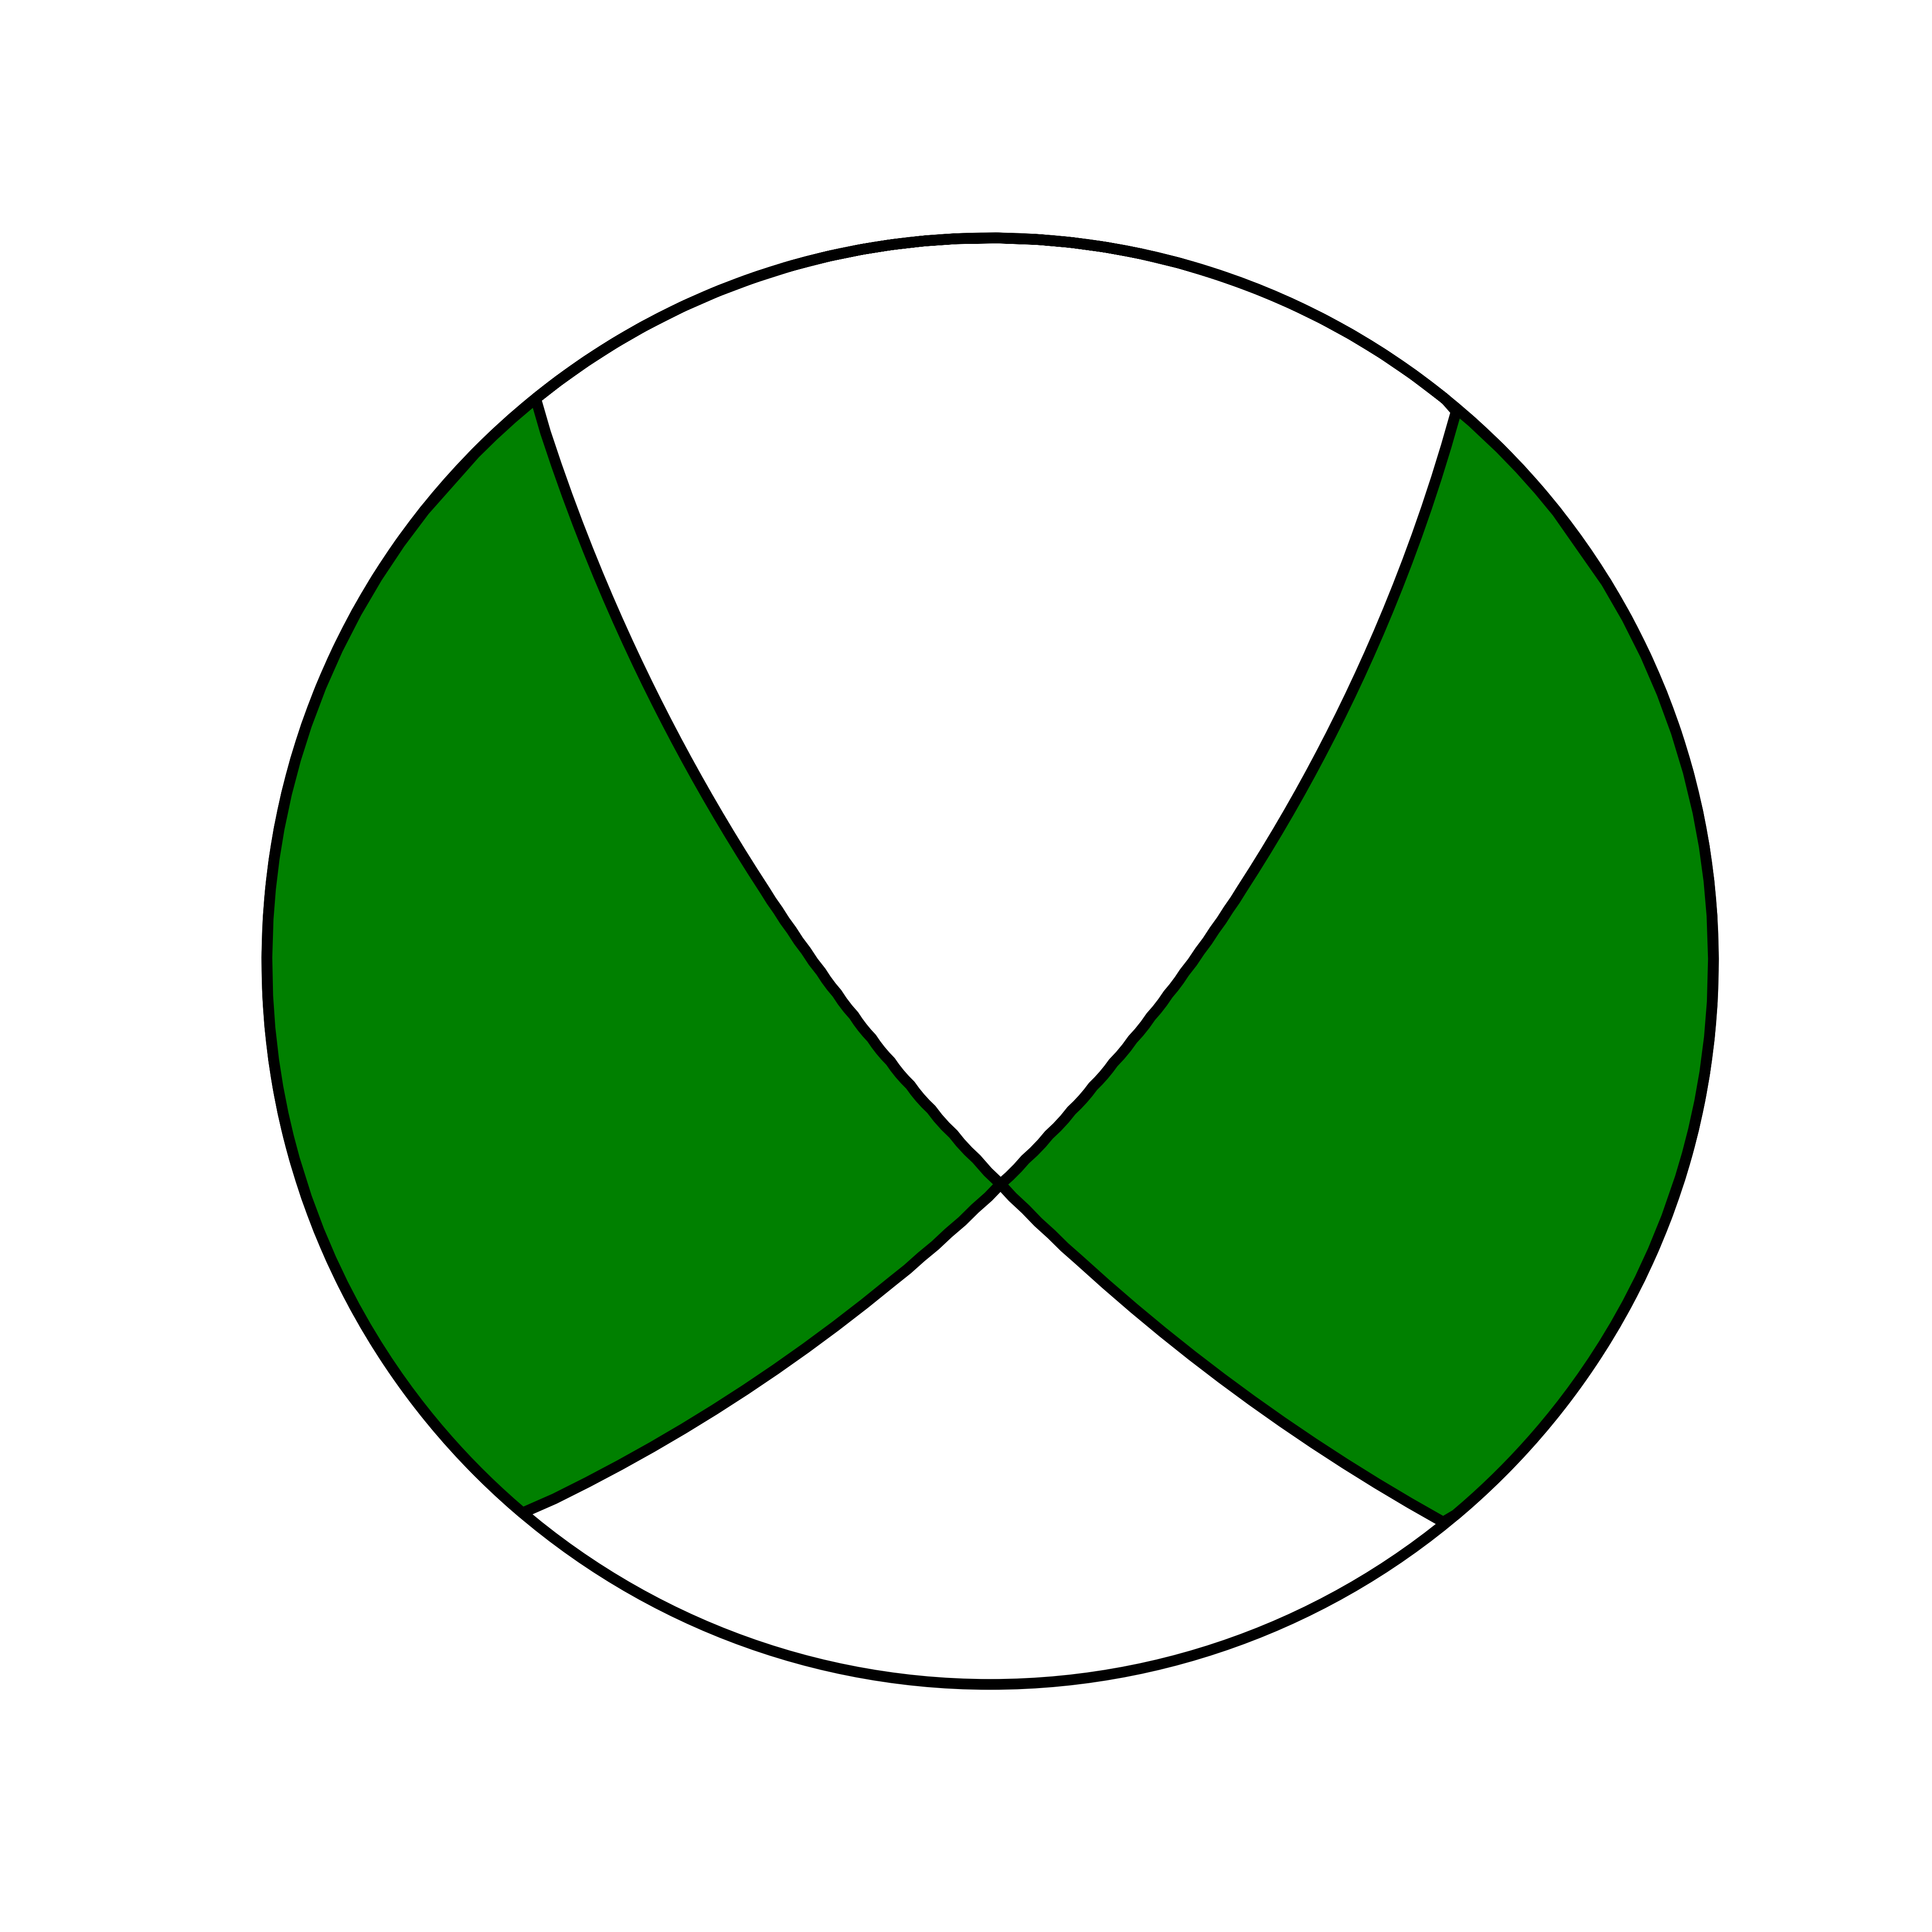
\includegraphics[width=0.1\textwidth]{source/table_yangbi/P_FM.png} \\
    
    CAP &  6.4 $M_{s}$ & 25.67/99.87 & 5.0 & 135/75/-168 42/78/-15 & NO & \includegraphics[width=0.1\textwidth]{source/table_yangbi/CAP.png} \\
    
    MCMTpy & 6.65 $M_{w}$ & 25.65/99.93 & 5.1 & 138/72/-170 45/80/-18  & 82 & \includegraphics[width=0.1\textwidth]{source/table_yangbi/MCMTpy.png} \\
    
    \bottomrule
  \end{tabular}
  \note{注:P Wave First Motion 和 CAP的结果来自中国地震局}
\end{table}


\subsection{矩张量反演}

在大多数情况下,天然地震的震源机制主要由双力偶成分组成;当地震破裂较为复杂时,例如多个子断层同时破裂,
震源机制中的非双力偶成为就不可忽略,例如CLVD成分。
因此我们进一步进行矩张量的反演,来验证漾濞地震是否含有较强的CLVD成分。
我们选取双力偶模型的MAP(最大后验概率)采样结果作为矩张量反演的初始模型。
我们使用20条马尔科夫链同时进行采样,每条马尔科夫链进行20000次采样,大约需要15个小时在CentOS Linux system (2.30 GHz Intel Xeon Gold 5218 CPU)操作系统上。
我们发现误差曲线继续下降,这表明地震包含非双力偶的成分,矩张量反演能更好的拟合波形(图~\ref{fig:misfit-yangbi-mt})。
矩张量反演的波形拟合互相关系数略高于双力偶模型反演的结果(图~\ref{fig:waveform-yangbi-mt})。
我们把所有矩张量解画在同一个沙滩球上(图~\ref{fig:Hudson}),并通过Hudson图展示所有解的偏离情况(图~\ref{fig:Hudson})。
Lune图是另外一种更直观的显示不同震源成分的可视化方法\citep{Tape2012},
我们将矩张量解的不确定性在基本Lune图上进行展示(图~\ref{fig:lune-yangbi} )。
Global CMT给出的非双力偶成分大约为 38\%,USGS给出的非双力偶成分大约为 7\%,
我们的结果,根据Jost\citep{Jost1989}定义的非双力偶,是18\%。


\begin{figure}[h]
    \centering
    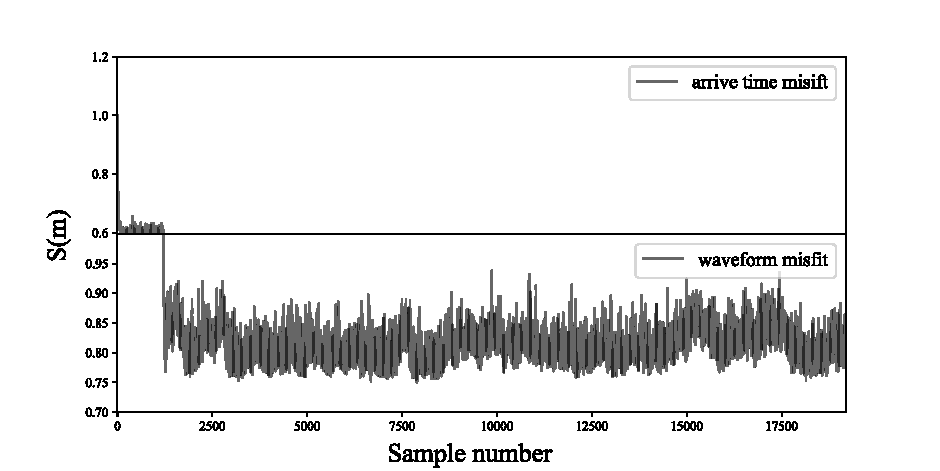
\includegraphics[width=0.9\textwidth]{source/misfit-yangbi-mt.pdf}
    \caption{漾濞地震矩张量模型反演的误差曲线}
    \label{fig:misfit-yangbi-mt}
    % \note{注:图注的内容不宜放到图题中。}
\end{figure}



\begin{figure}[h]
    \centering
    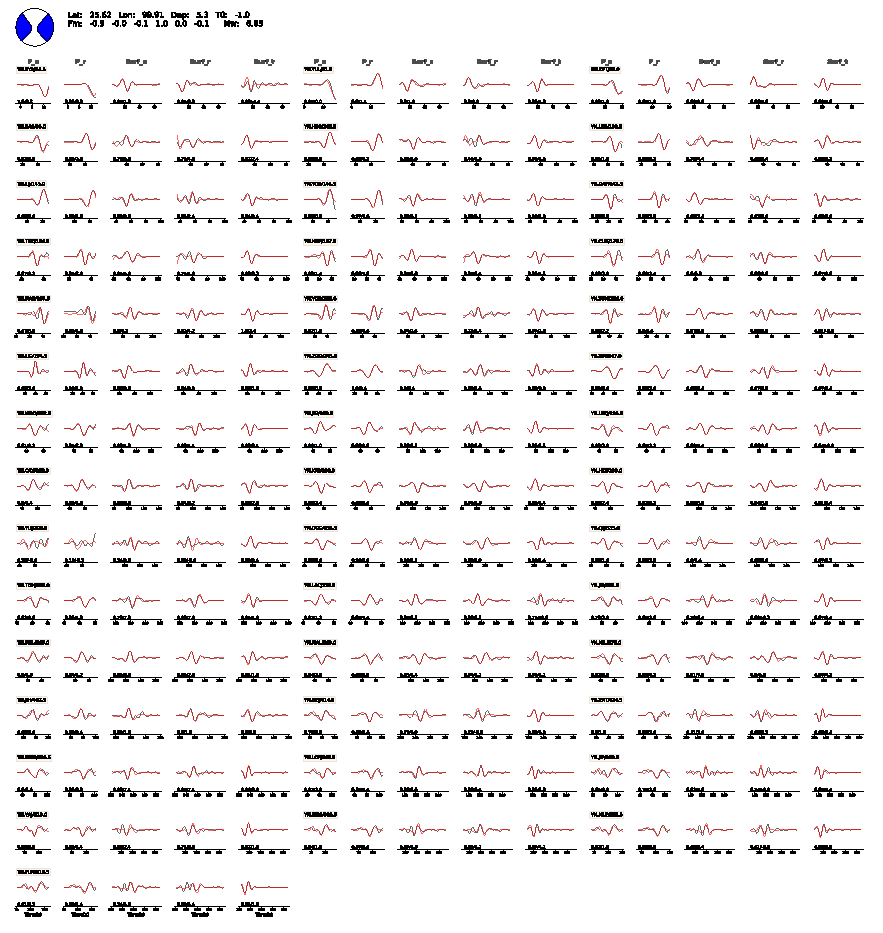
\includegraphics[width=0.9\textwidth]{source/waveform-yangbi-mt.pdf}
    \caption{漾濞地震矩张量模型反演的波形拟合图}
    \label{fig:waveform-yangbi-mt}
    \note{注:观测的地震波形用灰色线表示,合成的理论波形用红线表示;
    相关系数与时间偏移量在每个子图的左下方表示;
    每个台站的标注都由台网名称、台站名称和震中距组成;
    图中P\_z和P\_r分别表示P波的Z和R分量;
    Surf\_z、Surf\_r、Surf\_t分别表示面波的Z、R和T分量。}
\end{figure}


\begin{figure}[h]
    \centering
    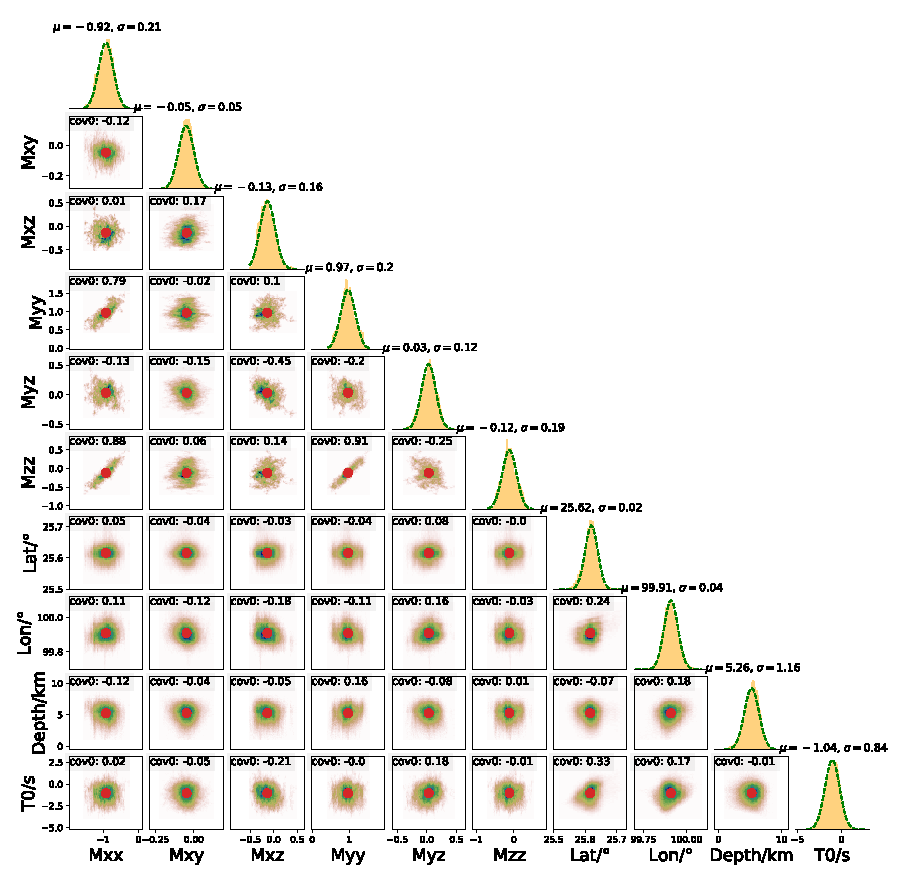
\includegraphics[width=0.9\textwidth]{source/hist-yangbi-mt.pdf}
    \caption{漾濞地震矩张量模型反演的后验概率分布}
    \label{fig:hist-yangbi-mt}
    \note{注:$\mu$和$\sigma$分别表示一维直方图的均值与标准差;
    绿色虚线表示最佳的高斯拟合分布;
    红色点表示MAP解;
    后验分布的协方差系数显示在对应子图的左上方。}
\end{figure}



\begin{figure}[h]
    \centering
    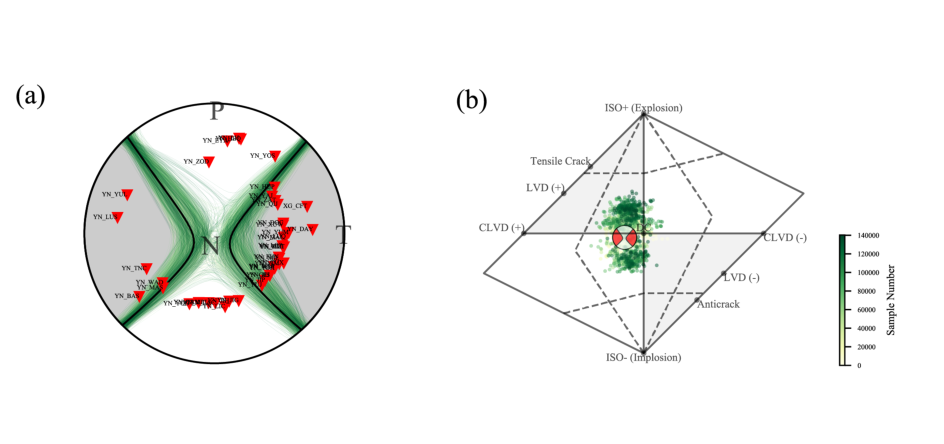
\includegraphics[width=0.9\textwidth]{source/Hudson.pdf}
    \caption{漾濞地震矩张量模型反演的Hudson图}
    \label{fig:Hudson}
    \note{注:(a)图为矩张量解(绿色线)的合集,黑色线表示MAP解,红色三角形台站在沙滩球上的分布,是使用等面积投影。(b)图是Hudson图,红色的沙滩球表示MAP解。}
\end{figure}


\begin{figure}[h]
    \centering
    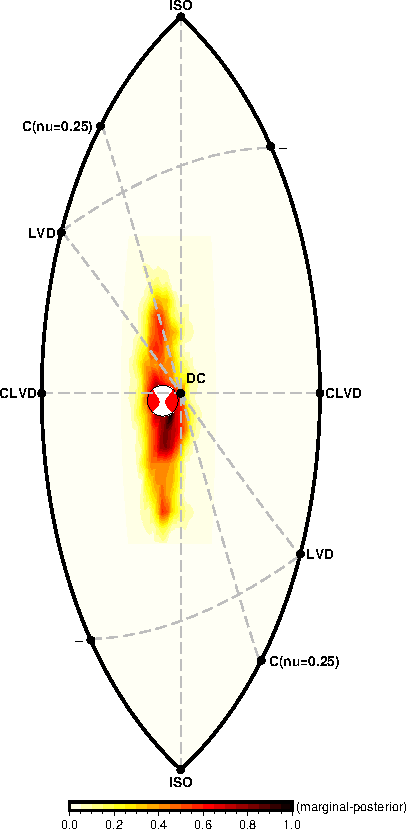
\includegraphics[width=0.5\textwidth]{source/lune-yangbi.pdf}
    \caption{漾濞地震矩张量模型反演的Lune图}
    \label{fig:lune-yangbi}
    \note{注:边缘后验概率在基本lune上的分布,红色沙滩球表示MAP解。}
\end{figure}



\section{2008年美国Mt. Carmel地震反演}

2008年4月18号,Mt. Carmel 地震发生在美国伊利诺斯州的东南方,靠近Wabash Valley seismic zone(WVSZ)地震带的北端(图~\ref{fig:map-us})。
我们从Incorporated Research Institutions for Seismology (IRIS)上获取三分量宽频带的地震波形数据。
在去除仪器响应后,我们挑选了8个高信噪比的台站,并将其地震记录转换到速度记录用于后续反演。
我们采用CUS velocity model\citep{Herrmann1979}作为计算一维格林函数的速度模型。

\begin{figure}[h]
    \centering
    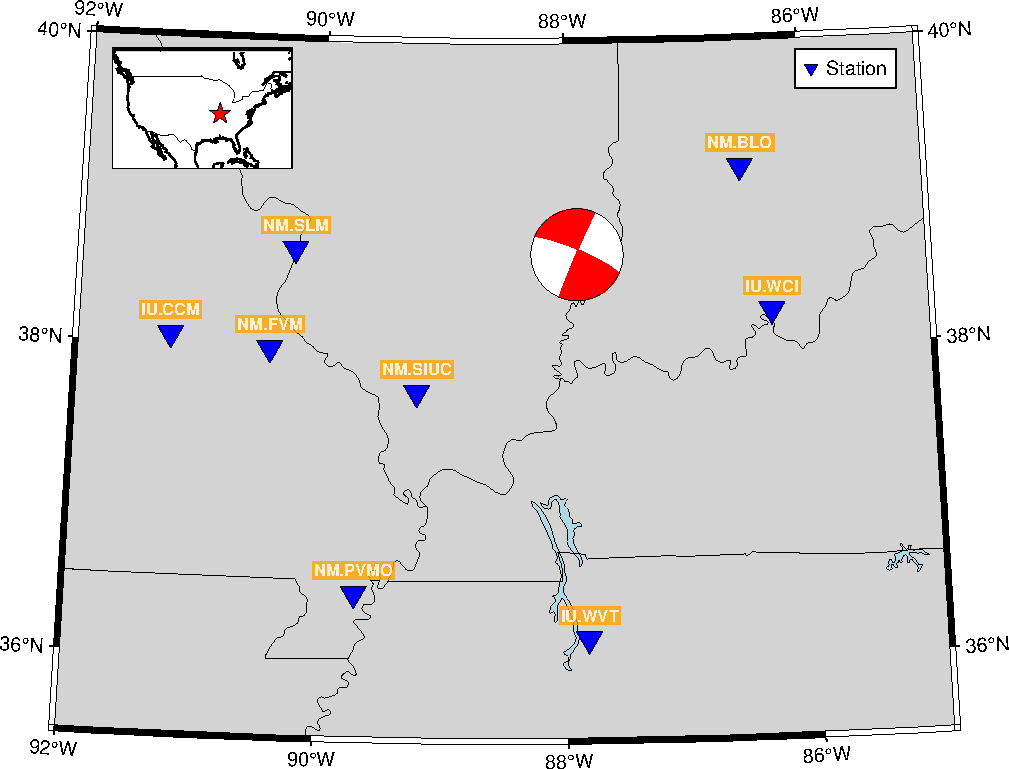
\includegraphics[width=0.9\textwidth]{source/map-us.pdf}
    \caption{美国Mt. Carmel地震的台站分布}
    \label{fig:map-us}
    \note{注:左上方子图的红色五角星显示研究区域。}
\end{figure}



\subsection{双力偶反演}

我们选取CAP的结果\citep{He2018}作为初始模型。
我们将地震波形数据分为为$Pnl$波和面波,用于后验概率采样。
对于$Pnl$波,我们设置滤波范围为0.05 - 0.25Hz,时间拟合窗口为P波相位到时的前2秒与后8秒。
对于面波,我们设置滤波范围为0.02 - 0.2Hz,时间拟合窗口为S波相位到时的前5秒与后25秒。
所有台站和相位的权重都设置成1。
为了避免因为cycle skipping现象陷入局部极小值,我们严格设置了滑动窗口在相应地震记录半个波长内。
我们估计相位到时的不确定性为0.3秒,波形的不确定性为0.015$cm/s$,我们设置参数$K_n$等于2000。
根据公式~\ref{equ:duration-time} 我们设置震源持续时间为2秒。

不同机构提供了不同的震源参数反演结果,见表~\ref{tab:us-1}。
双力偶的采样结果见图~\ref{fig:misfit-us-dc}(误差下降图)、图~\ref{fig:hist-us-dc}(后验概率分布图)、图~\ref{fig:waveform-us-dc}(波形拟合图),其中反演得到的纬度38.45°,经度-87.90°,strike 294°,dip 81°,rake 2°,与USGS的结果接近。
与USGS机构提供的震源深度25km相比,我们的结果显示了一个更浅的震源深度,为15.45km。
MCMTpy反演的震级为$M_w 5.26$,CAP的震级结果为$M_w 5.24$\citep{He2018},Global CMT的结果为$M_w 5.3$,三者较为一致。
我们使用单条马尔科夫链进行采样,大约需要2小时在CentOS Linux system (2.30 GHz Intel Xeon Gold 5218 CPU)操作系统上。

\begin{figure}[h]
    \centering
    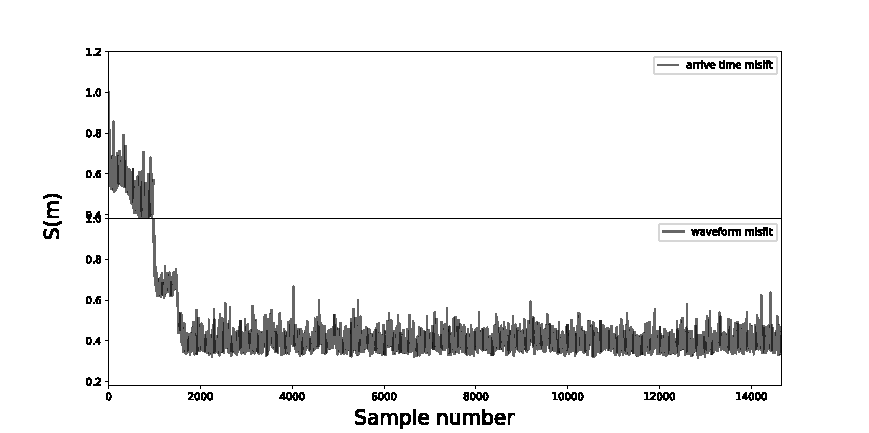
\includegraphics[width=0.9\textwidth]{source/misfit-us-dc.pdf}
    \caption{美国Mt. Carmel地震双力偶模型反演的误差图}
    \label{fig:misfit-us-dc}
    \note{注:两个阶段的误差函数都经过归一化处理。}
\end{figure}

\begin{figure}[h]
    \centering
    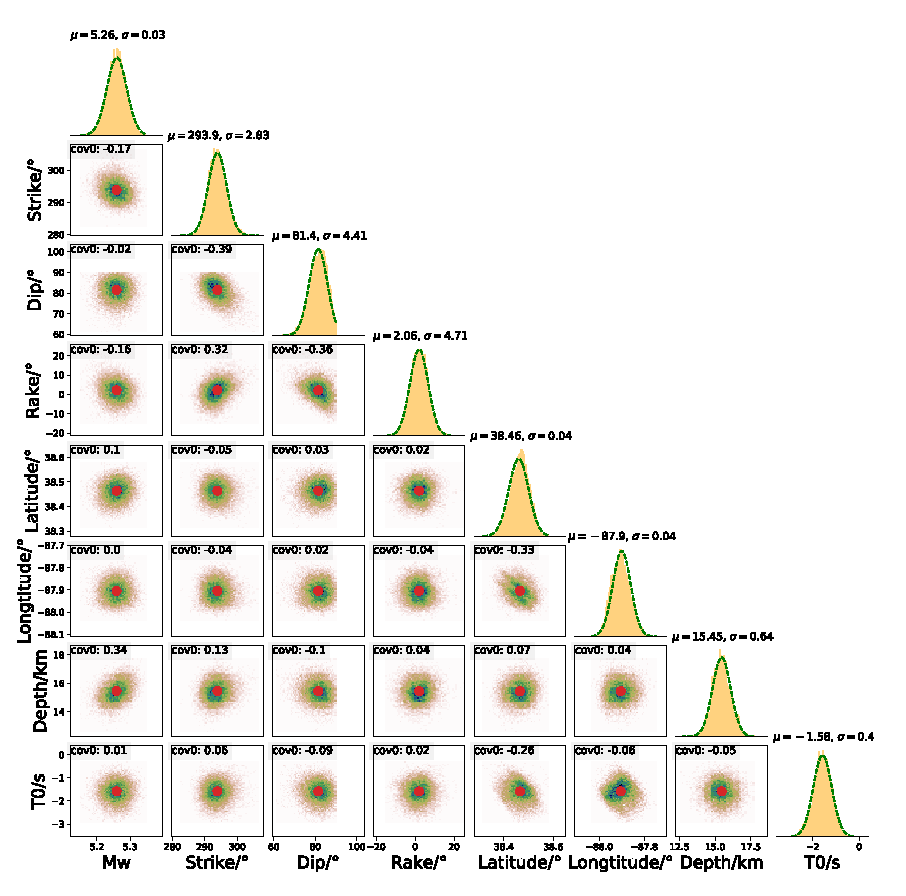
\includegraphics[width=0.9\textwidth]{source/hist-us-dc.pdf}
    \caption{美国Mt. Carmel地震双力偶模型反演的后验概率分布}
    \label{fig:hist-us-dc}
    \note{注:$\mu$和$\sigma$分别表示一维直方图的均值与标准差;
    绿色虚线表示最佳的高斯拟合分布;
    红色点表示MAP解;
    后验分布的协方差系数显示在对应子图的左上方。}
\end{figure}


\begin{figure}[h]
    \centering
    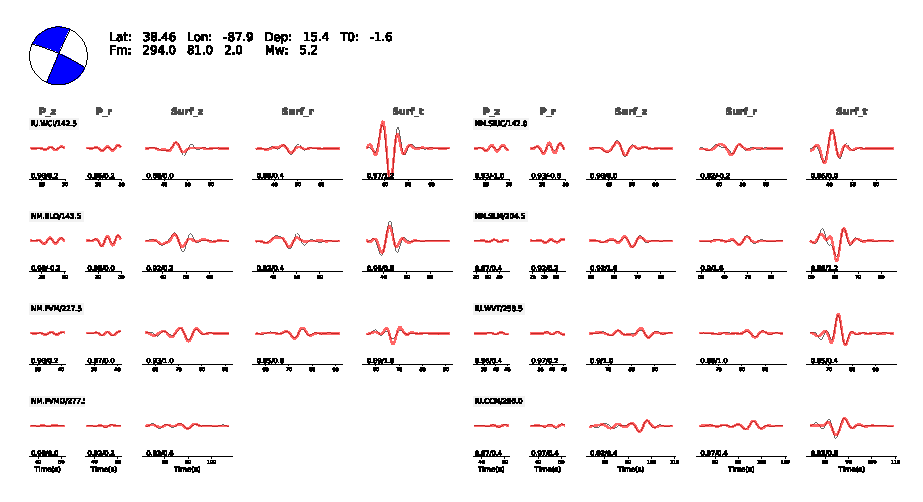
\includegraphics[width=0.9\textwidth]{source/waveform-us-dc.pdf}
    \caption{美国Mt. Carmel地震双力偶模型反演的波形拟合图}
    \label{fig:waveform-us-dc}
    \note{注:观测的地震波形用灰色线表示,合成的理论波形用红线表示;
    相关系数与时间偏移量在每个子图的左下方表示;
    每个台站的标注都由台网名称、台站名称和震中距组成;
    图中P\_z和P\_r分别表示P波的Z和R分量;
    Surf\_z、Surf\_r、Surf\_t分别表示面波的Z、R和T分量。}
\end{figure}



\begin{table}[h]
    \centering
    \caption{Source Parameters in 2008 Mt. Carmel Earthquake of Different Agencies}
    \label{tab:us-1}
  %   \begin{tabular}{c|cccp{6em}p{3em}c}
      \centering%把表居中
      \begin{tabular}{m{2cm}<{\centering}m{1.5cm}<{\centering}m{2cm}<{\centering}m{1cm}<{\centering}m{2cm}<{\centering}m{1cm}<{\centering}m{2cm}<{\centering}}
  
      \toprule
      Method   & Mag & Lat/Lon & Depth & Plane 1 and 2 (strike/dip/rake) & Percent DC(\%) & Beachball    \\
  
      \midrule
      Global CMT &  5.3 $M_{w}$ & 38.49/-87.86 & 26.9 & 295/88/1 205/89/178 & 89 & \includegraphics[width=0.1\textwidth]{source/table_us/G_CMT.png} \\
      
      USGS W-phase & 5.44 $M_{w}$ & 38.45/-87.89 & 26.9 & 295/88/1 205/89/178 & 89 & \includegraphics[width=0.1\textwidth]{source/table_us/USGS_W.png} \\
      
      CAP &  5.24 $M_{w}$ & 38.45/-87.89 & 16.0 & 297/84/1 206/89/173 & NO & \includegraphics[width=0.1\textwidth]{source/table_us/CAP.png} \\
      
      MCMTpy & 5.26 $M_{w}$ & 38.46/-87.90 & 15.45 & 294/81/2 204/88/171  & 67 & \includegraphics[width=0.1\textwidth]{source/table_us/MCMTpy.png} \\
      
      \bottomrule
    \end{tabular}
    \note{注:CAP的结果来自He(2018)}
\end{table}



\subsection{矩张量反演}

我们选取双力偶模型的MAP(最大后验概率)采样结果作为矩张量反演的初始模型。
我们使用20条马尔科夫链同时进行采样,每条马尔科夫链进行20000次采样,大约需要2个小时在CentOS Linux system (2.30 GHz Intel Xeon Gold 5218 CPU)操作系统上。

图~\ref{fig:hist-us-mt}表示矩张量模型下的后验概率分布,Lune图~\ref{fig:lune-us}表示矩张量解的不确定性。
我们发现美国Mt. Carmel地震显示出较复杂震源成分,USGS机构给的非双力偶成分为11\%,
作为对比我们的结果显示非双力偶成分高达37\%,可能的原因此次地震破裂的断层较为复杂。

\begin{figure}[h]
    \centering
    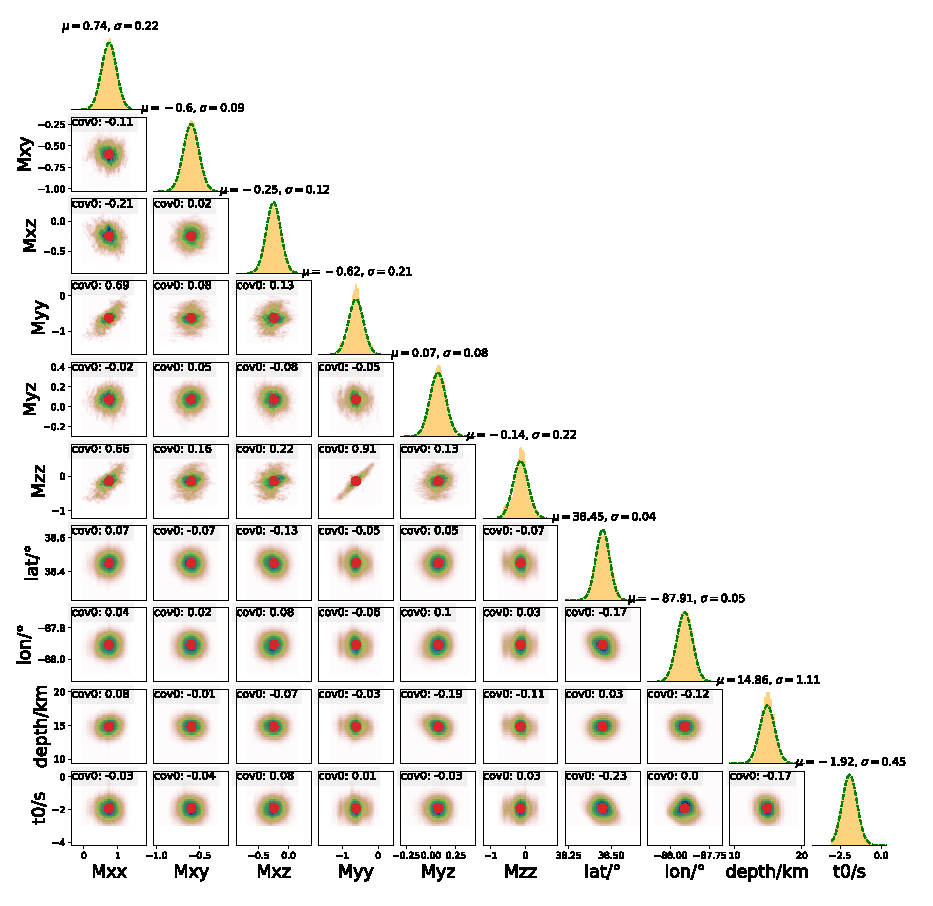
\includegraphics[width=0.9\textwidth]{source/hist-us-mt.pdf}
    \caption{美国Mt. Carmel地震矩张量模型反演的后验概率分布}
    \label{fig:hist-us-mt}
    \note{注:$\mu$和$\sigma$分别表示一维直方图的均值与标准差;
    绿色虚线表示最佳的高斯拟合分布;
    红色点表示MAP解;
    后验分布的协方差系数显示在对应子图的左上方。}
\end{figure}



\begin{figure}[h]
    \centering
    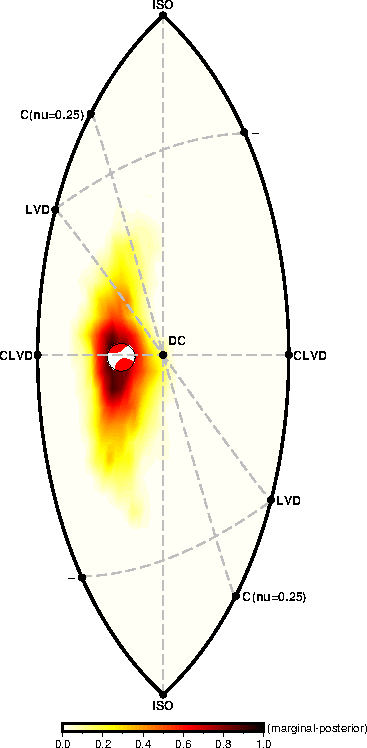
\includegraphics[width=0.5\textwidth]{source/lune-us.pdf}
    \caption{美国Mt. Carmel地震矩张量模型反演的Lune图}
    \label{fig:lune-us}
    \note{注:边缘后验概率在基本lune上的分布,红色沙滩球表示MAP解。}
\end{figure}

\section{讨论}

\subsection{去除累积误差}

传统的基于射线追踪的地震定位方法,定位结果通常是地震破裂的初始点,并不是地震破裂的矩中心。
地震矩中心与初始破裂点的位置偏差通常是由于地震破裂的方向性导致的\citep{Xu2019,Li2020}。
之前的研究\citep{Tan2018}发现震源位置的偏差会对震源机制反演的结果造成较大影响。
而传统的两步法,先进行地震定位再进行震源机制反演,毫无疑问会受到累计误差的影响。
第一步地震定位的误差会传递到第二步震源机制反演中,从而影响最终的反演结果。
因为,同时进行地震定位与震源机制反演是十分有必要的。

但是,当我们没有地震位置的明确先验信息时,只使用波形误差函数进行反演采样,非常容易陷入局部极小值。
这是因为我们使用了错误的时间拟合窗口,从而引起了circle skipping的现象。
因此拥有一个同时进行震源参数反演(地震定位与震源机制反演)的代码是较为困难的。
一个合适的策略是先确定一个粗略的地震位置,然后在该位置附近同时搜索最优地震位置与震源机制解。
得益于马尔科夫链的性质,即当前系统的状态仅依赖于系统的上一个状态,这让同时进行地震定位与震源机制反演成为可能。
在第一个阶段,新方法使用相位到时信息去粗略估计震源位置;然后在第二个阶段,马尔科夫链会使用第一个阶段最新的或者MAP解,
并利用波形信息误差函数去同时估计震源机制与地震位置。
因为在第二阶段同时进行了地震定位与震源机制反演,所以新方法可以有效去除震源位置带来的累计误差。
在漾濞地震中,我们发现MCMTpy的结果与传统两步法的结果显示出了位置上较小的差异。
我们发现MCMTpy进行波形拟合的平均互相关系数是0.89,而CAP的方法显示为0.88。
两种方法的互相关系数的差异较小,这可能是由于两种方法反演的震源深度较为接近。
相比地震水平位置,地震波形对震源深度更加敏感。
当地震位置偏差较为明显、用更高频率的波形去拟合数据时,这种差异性会更加明显。



\subsection{时间偏移与地震位置的关系}

不准确的速度模型在地震震源反演问题中是不可避免的。通常,速度模型造成的系统偏差表现在两个方面:
波形相位的整体偏移与随着震中距的线性偏移。
同时由于三维速度模型的效应,会造成波形相位的随机偏差。

时间偏移量$\delta t$是考虑到速度模型的不准确定而引入的,被广泛使用在震源参数反演问题中,例如经典的CAP方法\citep{Zhu1996}。
直觉上,允许时间偏移会对地震定位造成一定影响,然而我们在第二阶段使用的误差函数(方程~\ref{equ:misfit-function-2}),是仅使用波形的振幅信息去反演震源机制的。
虽然地震位置的信息能同时影响地震波形的形状与振幅,但当时间偏移量足够弥补速度模型不准带来的偏差时,最优的震源位置对应的误差始终是最小的。
允许时间偏移虽然扩大了搜索范围,但不会产生更多波形失配函数的局部最小值。
因此,我们相信允许时间偏移不会影响震源定位的精度。

我们选取漾濞地震中所有台站中相关系数高于0.8的时间偏移(图~\ref{fig:timeshift}),我们发现这些时间偏移量具有明显的整体偏移特点(大多数时间偏移量大于0秒),
并且有随震中距呈线性增大的趋势。
最主要的时间偏移量集中在0 - 4 秒,并且我们发现时间偏移量在每个台站都具有明显的差异性,这表明速度模型的3-D效应的存在。
考虑到我们使用的是中国西南的公共速度模型Community Velocity Model V.1.0 of Southwest China\citep{Liu2021},
这是一个复杂的三维速度模型,我们进行数值平均后变成一维速度模型。
在我们的研究区域速度模型的差异性能达到10\%,因此对速度模型进行1-D平均,很可能导致系统速度偏差。

\begin{figure}[h]
    \centering
    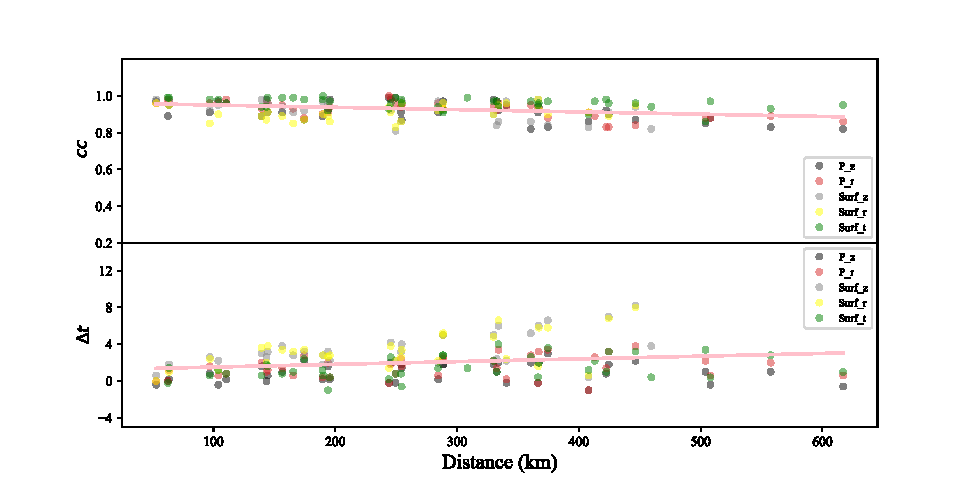
\includegraphics[width=0.9\textwidth]{source/timeshift.pdf}
    \caption{漾濞地震双力偶模型反演的时间偏移量}
    \label{fig:timeshift}
    \note{注:所有台站中相关系数大于0.8的时间偏移;粉色线表示时间偏移点的线性回归直线。}
\end{figure}



\subsection{先验模型的依赖性与限制性}

MCMC的算法通常对先验模型具有较强的依赖,其应用往往局限于较低维的问题\citep{Fang2019}。
我们的新方案MCMTpy能够有效的降低对先验信息的依赖。
在估计震源位置的第一阶段,即使我们没有明确的震源位置信息,但因为我们只需要反演四个参数(纬度、经度、深度、发震时刻),
其维数较低,所以我们也能很快的获得震源位置的后验概率密度PDD。
在第二个阶段,我们需要同时估计震源机制与震源位置,尽管模型参数的维数在增加,但因为我们从第一阶段获得了震源位置的先验信息,
所以我们也能够较快的获得后验概率分布。
MCMTpy的另一个优点是,其作为一种全局优化算法,能够有效避免陷入局部极小值,但是如果模型空间中存在势垒点(barrier minima),该方法也会失效。
我们使用30个随机初始模型与一次网格搜索实验进行双力偶模型采样,进而验证MCMTpy的鲁棒性。

首先,我们固定dip角度为72°,使用网格搜索计算了strike - rake的二维解空间。
图~\ref{fig:grid-search}显示了网格搜索的结果。
我们可以清楚的发现二维解空间存在6个极小值,因为strike与rake角度存在周期性的性质,实际存在4个极小值,
分别位于F1(strike 138° 和 rake -171°)、F2(strike 45° 和 rake -12°)、E1(strike 316° 和 rake -176°)和E2(strike 225° 和 rake -7°)附近。
事实上,F1和F2是一对共轭解平面的解,E1和E2是另一对共轭解平面的解。
我们发现F1和E1的strike角度存在一个180°的差异,对应于断层走向两个相反的角度。
在测线A1 - A2中,我们发现一些明显的局部极小值,例如LM点;还有两个明显的极小值点F1和E1。
其中F1是全局最小值点,E1极小值点我们称之为势垒点。
势垒点的存在会严重影响反演结果,一旦陷入势垒点,马尔科夫链很难跳出去所有全局极小值。

我们在整个模型参数空间生成30个随机的初始模型,主要参数包括震级、strike、dip、rake、纬度、经度、深度、发震偏移时间。
图~\ref{fig:randFM}显示了30个不同的初始模型采样的结果(其中第4、12、15次实验的初始模型靠近格林函数库的边界,在随机搜索时超出了搜索边界并终止搜索,所以没有参与下面的计算)。
我们可以清晰发现有4组解,这四组解的平均值等详细信息可以在表~\ref{tab:yangbi-2}查看。
我们发现了一下几点:
\begin{enumerate}
    \item 每组解内的震级、纬度、经度、深度和发震时刻都非常接近。这表明新方法可以有效的收敛,并不受初始模型的影响。
    \item strike与rake角度显示出4组不同的解,同时4组解的dip角度都是大约72°,正好对应网格搜索结果的F1、F2、E1和E2点。
    \item Global CMT的结果与E1点的结果非常接近,他们的strike角度都是315°左右,这表明Global CMT的解很可能陷入了E1势垒点的局部极小值中。
\end{enumerate}

上述结果表明新方法可以有效地减小初始模型的依赖性,并能突破局部极小值(例如 LM点)的限制,但当遇到势垒点时,该方法也无能为力。

\begin{table}[h]
    \centering
    \caption{Source Parameters of 30 Random Initial Models}
    \label{tab:yangbi-2}
  %   \begin{tabular}{c|cccp{6em}p{3em}c}
      \centering%把表居中
      \begin{tabular}{m{1.5cm}<{\centering}m{1.5cm}<{\centering}m{2cm}<{\centering}m{1cm}<{\centering}m{2cm}<{\centering}m{1cm}<{\centering}m{2cm}<{\centering}}
  
      \toprule
      Solution   & Mag & Lat/Lon & Depth & Strike/Dip/Rake & T0 & Beachball    \\
  
      \midrule
      F1 & 6.64 & 25.65/99.93 & 4.90 & 138/74/-171 & -0.56 & 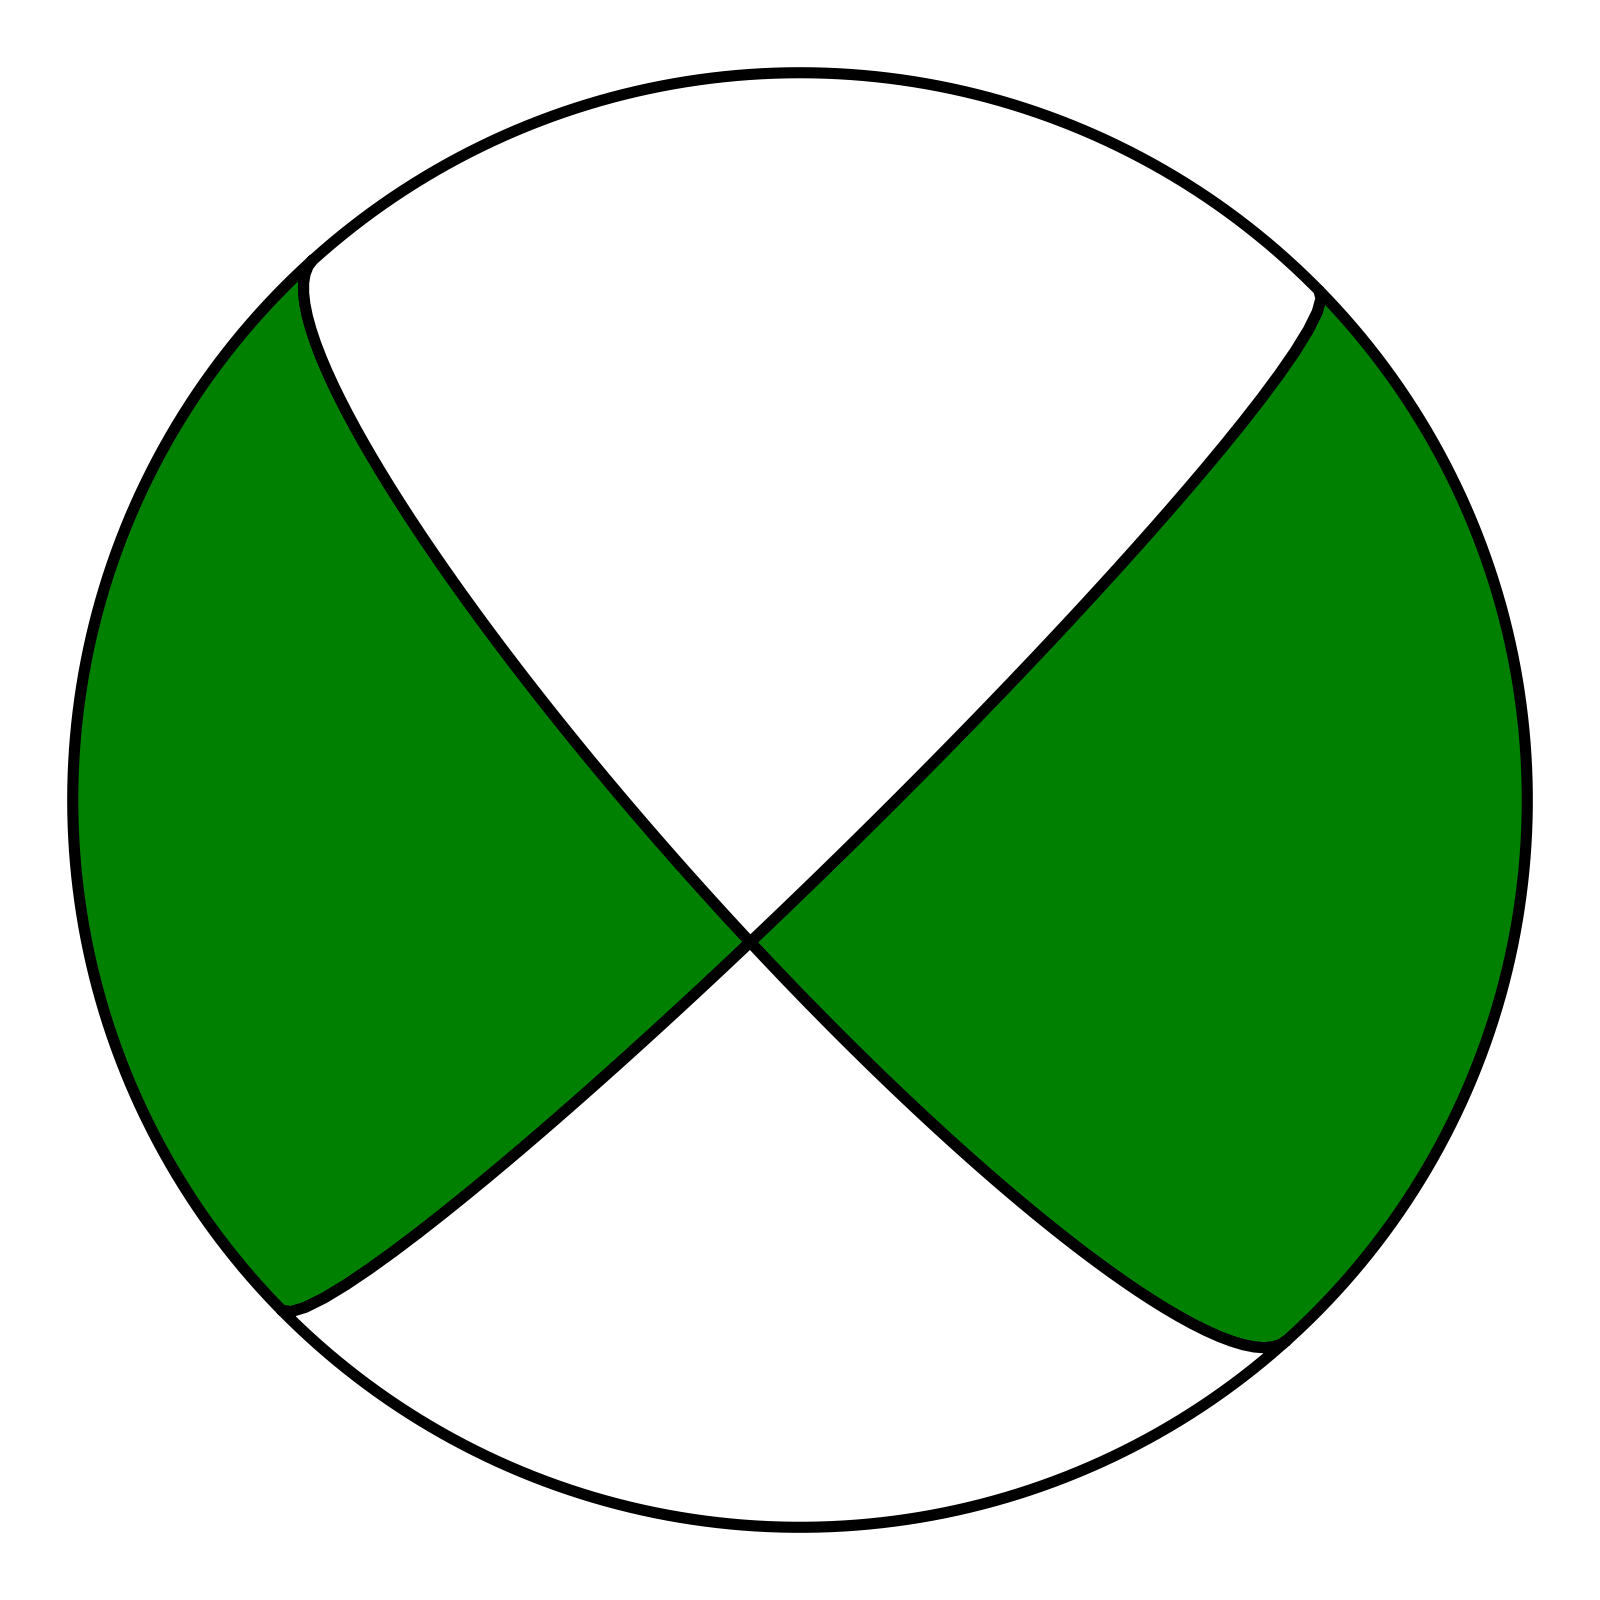
\includegraphics[width=0.1\textwidth]{source/table_randFM/FM1.png} \\
      
      F2 & 6.64 & 25.64/99.93 & 4.98 & 45/79/-12 & -0.85 & 
\includegraphics[width=0.1\textwidth]{source/table_randFM/FM2.png} \\
      
      E1 & 6.64 & 25.64/99.91 & 4.84 & 316/76/-176 & -1.17 & 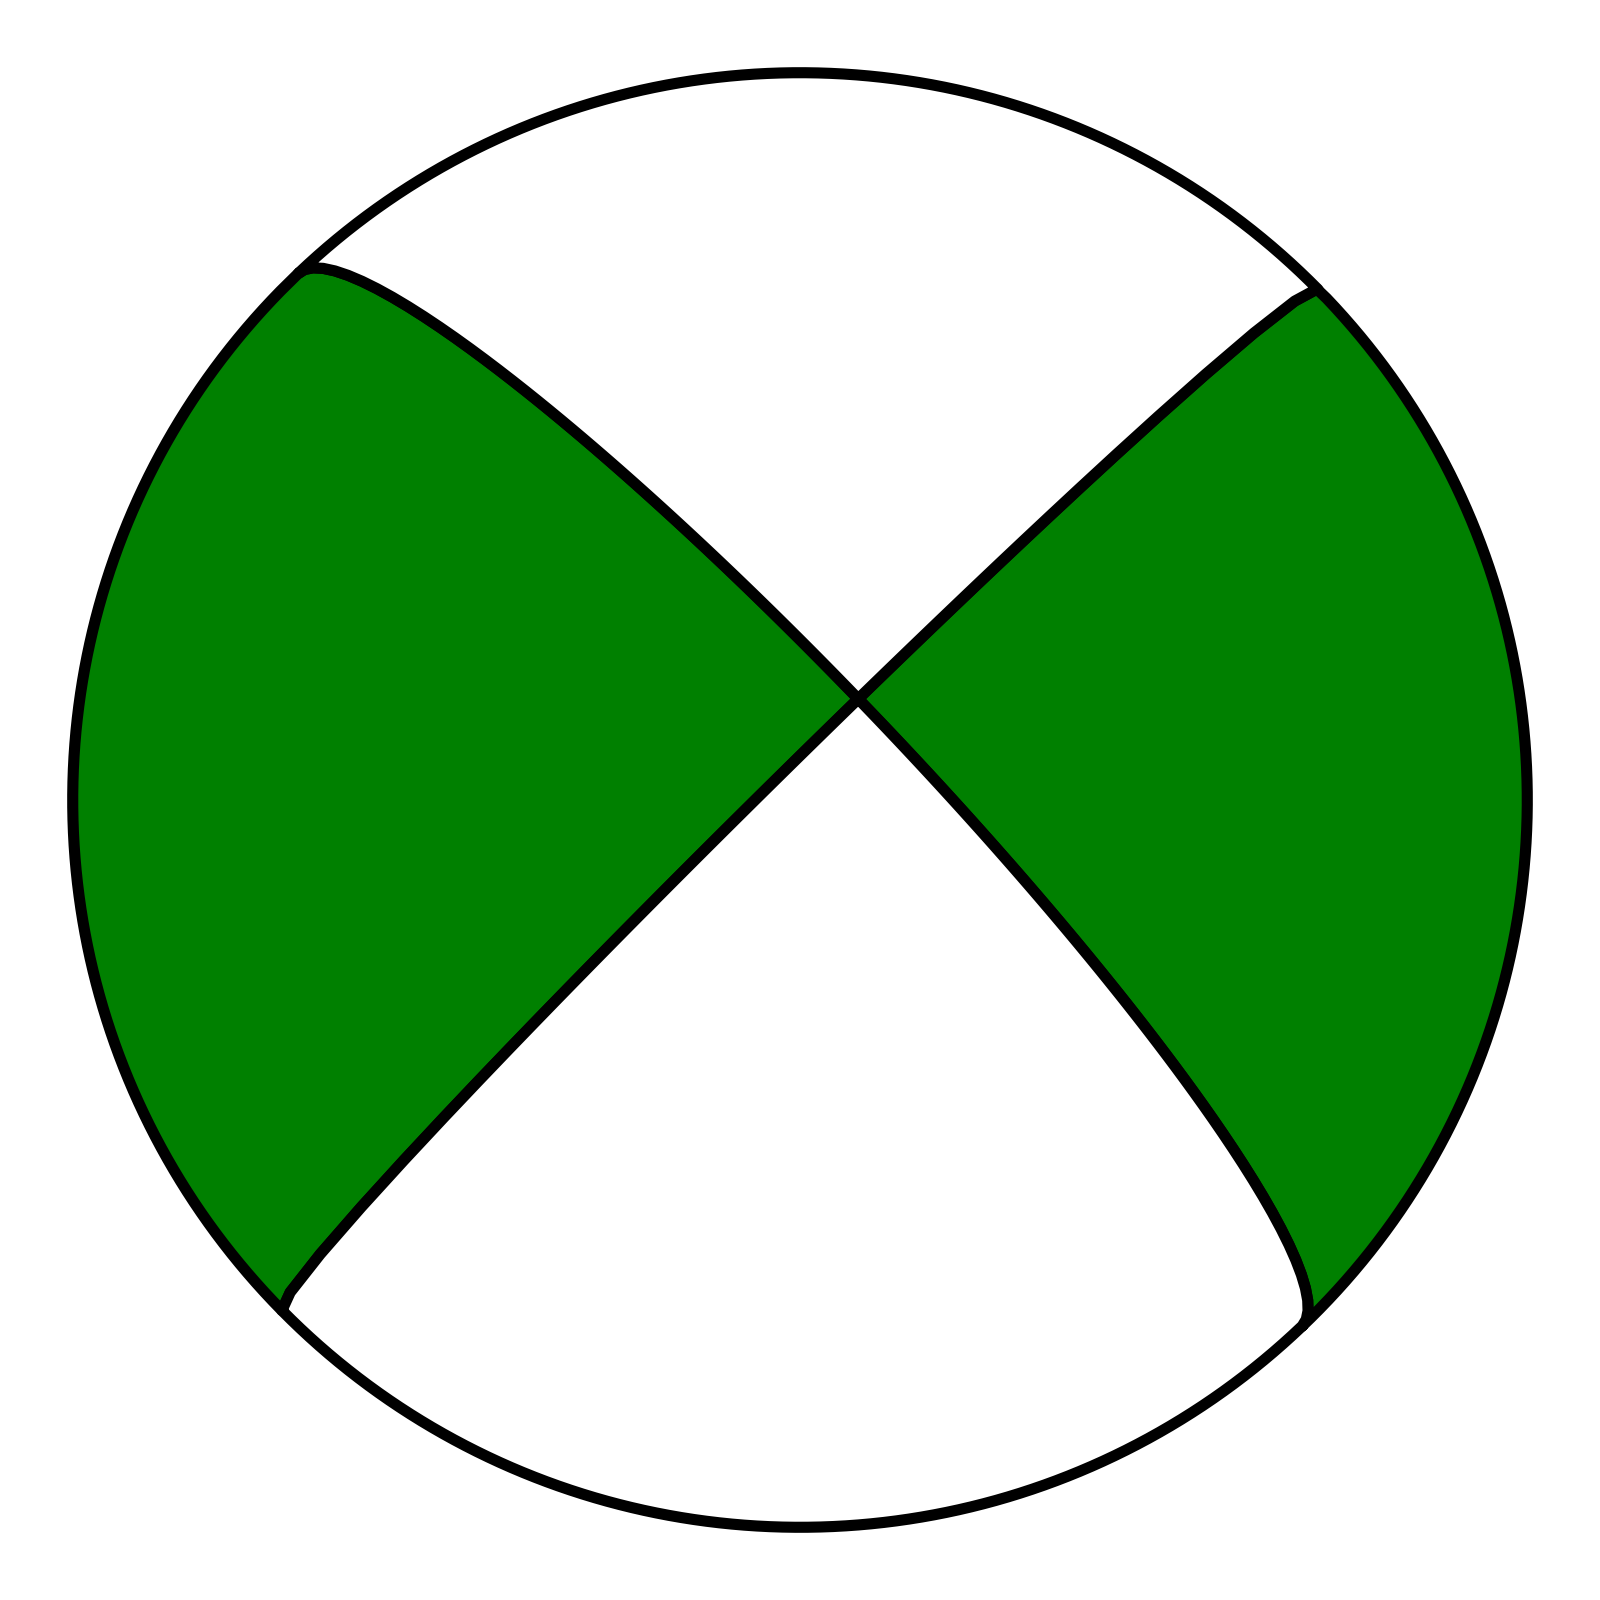
\includegraphics[width=0.1\textwidth]{source/table_randFM/LM1.png} \\
      
      E2 & 6.43 & 25.64/99.92 & 4.59 & 225/80/-7 &  -0.87 & 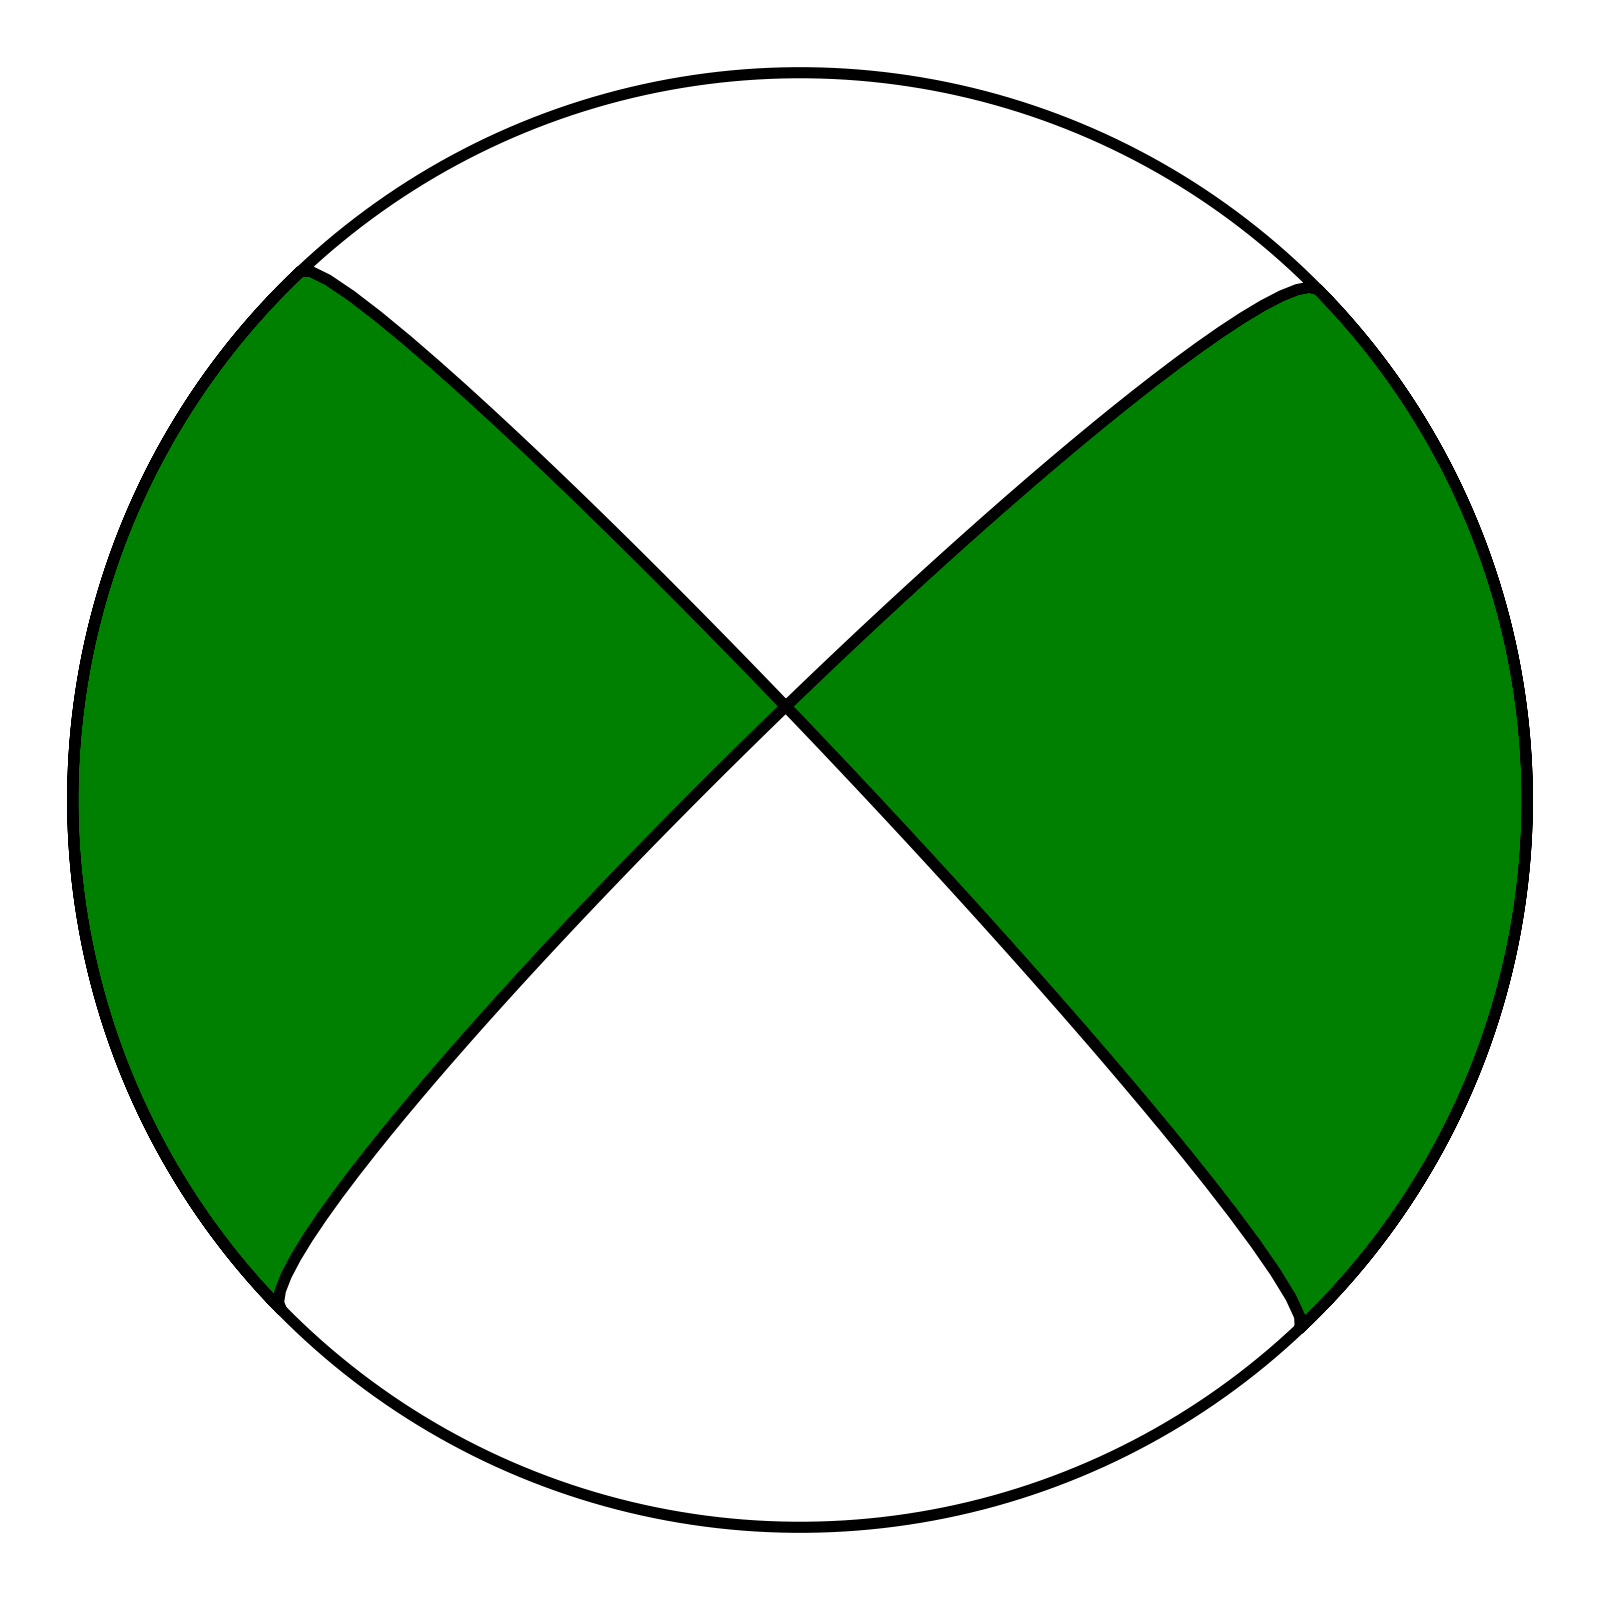
\includegraphics[width=0.1\textwidth]{source/table_randFM/LM2.png} \\
      
      \bottomrule
    \end{tabular}
    \note{注:第4、12、15次实验的初始模型靠近格林函数库的边界,在随机搜索时超出了搜索边界并终止搜索,所以没有参与计算。}
\end{table}

\begin{figure}[h]
    \centering
    \includegraphics[width=0.9\textwidth]{source/grid-search.pdf}
    \caption{漾濞地震strike - rake的网格搜索结果}
    \label{fig:grid-search}
    \note{注:绿色方框所示的LM点是一个局部极小值点示例,其在A1 - A2测线中也可以看到;
    黄色方框所示的F1和F2点一对共轭震源机制解;紫色方框所示的E1和E2点一对共轭势垒解;
    子图(b)和(c)分别是沿(a)图测线B1 - B2和A1 - A2的误差曲线。}
\end{figure}

\begin{figure}[h]
    \centering
    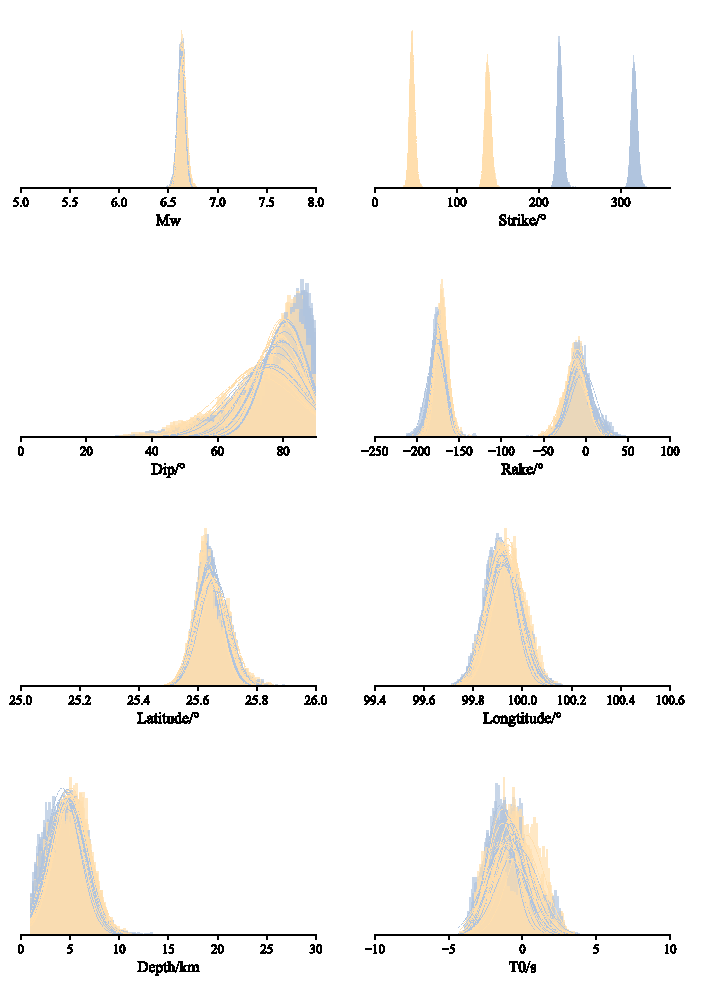
\includegraphics[width=0.9\textwidth]{source/randFM.pdf}
    \caption{漾濞地震中30组随机初始模型反演结果的后验概率分布}
    \label{fig:randFM}
    \note{注:所有的采样结果展示在同一张图片中;
    其中黄色的直方图表示一对共轭震源机制解;而蓝色的直方图表示陷入势垒点的震源机制解。}
\end{figure}



势垒点并不是存在于所有反演问题中,其依赖于具体的问题。
在我们的研究中,我们发现漾濞地震发生在一个大约呈72°左右的断层上,是一个走滑成分为主的地震,而势垒点恰好出现在沿着断层走向相反的方向上。
一种有效的突破势垒点的方法是使用网格搜索算法,其对所有非线性问题都有效,但其昂贵的计算代价限制了它在高维问题中的应用。
另外一种方法是像我们做的那样,生成多条马尔科夫链,使用不同的初始模型同时采样,然后选取后验概率空间中误差最小的解作为最终结果。
这种方案适用于我们的震源反演问题,但多条马尔科夫链的使用会增加计算量。
突破势垒点更有效的方法是使用并行退火\citep{Dosso2013}或模拟退火方法\citep{Billings1994}。
在这些方法中,为了提高搜索的效率,引入了可变的温度参数;但温度参数的选取并不是容易的操作,会严重影响最终的反演结果\citep{Dosso2013}。

\subsection{计算量要求}

在我们反演美国Mt. Carmel地震的示例中,我们使用8个台站的三分量数据,单次采样时间约为0.3秒在CentOS Linux system (2.30 GHz Intel Xeon Gold 5218 CPU)系统上,
然而精确的时间会随着硬件系统的不同而不同。
大约进行10000次采样就已经足够获得一个精确的后验概率分布了,此时后验概率的协方差系数不再发生显著地变化。
然后,MCMC的方法因为其随机采样的特点,其对高维模型空间采样的效率较低\citep{Fang2019}。
最近一些基于哈密顿系统特性进行蒙特卡洛采样的算法可以有效地提高采样接受率,
但其代价是需要计算参数的梯度信息(Fichtner and Simutė, 2018),而梯度信息的计算通常是非常昂贵的。
格林函数库的数据量通常很大,需要几个GBs的硬盘空间进行存储。




% \subsubsection{三级节标题}

% \paragraph{四级节标题}

% \subparagraph{五级节标题}